\documentclass[12pt,]{book}
\usepackage{lmodern}
\usepackage{amssymb,amsmath}
\usepackage{ifxetex,ifluatex}
\usepackage{fixltx2e} % provides \textsubscript
\ifnum 0\ifxetex 1\fi\ifluatex 1\fi=0 % if pdftex
  \usepackage[T1]{fontenc}
  \usepackage[utf8]{inputenc}
\else % if luatex or xelatex
  \ifxetex
    \usepackage{mathspec}
  \else
    \usepackage{fontspec}
  \fi
  \defaultfontfeatures{Ligatures=TeX,Scale=MatchLowercase}
\fi
% use upquote if available, for straight quotes in verbatim environments
\IfFileExists{upquote.sty}{\usepackage{upquote}}{}
% use microtype if available
\IfFileExists{microtype.sty}{%
\usepackage{microtype}
\UseMicrotypeSet[protrusion]{basicmath} % disable protrusion for tt fonts
}{}
\usepackage[margin=1in]{geometry}
\usepackage{hyperref}
\hypersetup{unicode=true,
            pdftitle={Challenges and Tools in the Assessment and Management of Pacific Salmon Fisheries},
            pdfauthor={Ben Staton},
            pdfborder={0 0 0},
            breaklinks=true}
\urlstyle{same}  % don't use monospace font for urls
\usepackage{natbib}
\bibliographystyle{myapalike}
\usepackage{longtable,booktabs}
\usepackage{graphicx,grffile}
\makeatletter
\def\maxwidth{\ifdim\Gin@nat@width>\linewidth\linewidth\else\Gin@nat@width\fi}
\def\maxheight{\ifdim\Gin@nat@height>\textheight\textheight\else\Gin@nat@height\fi}
\makeatother
% Scale images if necessary, so that they will not overflow the page
% margins by default, and it is still possible to overwrite the defaults
% using explicit options in \includegraphics[width, height, ...]{}
\setkeys{Gin}{width=\maxwidth,height=\maxheight,keepaspectratio}
\IfFileExists{parskip.sty}{%
\usepackage{parskip}
}{% else
\setlength{\parindent}{0pt}
\setlength{\parskip}{6pt plus 2pt minus 1pt}
}
\setlength{\emergencystretch}{3em}  % prevent overfull lines
\providecommand{\tightlist}{%
  \setlength{\itemsep}{0pt}\setlength{\parskip}{0pt}}
\setcounter{secnumdepth}{5}
% Redefines (sub)paragraphs to behave more like sections
\ifx\paragraph\undefined\else
\let\oldparagraph\paragraph
\renewcommand{\paragraph}[1]{\oldparagraph{#1}\mbox{}}
\fi
\ifx\subparagraph\undefined\else
\let\oldsubparagraph\subparagraph
\renewcommand{\subparagraph}[1]{\oldsubparagraph{#1}\mbox{}}
\fi

%%% Use protect on footnotes to avoid problems with footnotes in titles
\let\rmarkdownfootnote\footnote%
\def\footnote{\protect\rmarkdownfootnote}

%%% Change title format to be more compact
\usepackage{titling}

% Create subtitle command for use in maketitle
\newcommand{\subtitle}[1]{
  \posttitle{
    \begin{center}\large#1\end{center}
    }
}

\setlength{\droptitle}{-2em}

  \title{Challenges and Tools in the Assessment and Management of Pacific Salmon
Fisheries}
    \pretitle{\vspace{\droptitle}\centering\huge}
  \posttitle{\par}
    \author{Ben Staton}
    \preauthor{\centering\large\emph}
  \postauthor{\par}
    \date{}
    \predate{}\postdate{}
  
\usepackage{booktabs}
%%% This is an example file for the Auburn University style options
%%%       aums.sty (Masters Thesis)
%%%       auphd.sty (Ph.D. Dissertation)
%%%       auhonors.sty (Honors Scholar)

%%%To use it, please edit the necessary options, title, author, date, year, keywords, advisor, professor, etc. 

% \documentclass[12pt]{report}
\usepackage{setspace}
% \usepackage{titlesec}
%\setcounter{secnumdepth}{3}
% \usepackage{aums}       % For Master's papers
\usepackage{auphd}     % For Ph.D.
%\usepackage{auhonors}  % For honors college
\usepackage[normalem]{ulem}       % underlining on style-page; see \normalem below
\usepackage{url}
\usepackage[table]{xcolor}
\usepackage{tikz}
\usepackage{pgf}
\usepackage{color,soul}
\usepackage{float}
\usepackage{caption}
\captionsetup{width=\textwidth}

\usepackage{amsmath,amsthm, amsfonts, mathrsfs, graphicx, setspace, fullpage, color}
\usepackage{natbib, appendix}
\usepackage[T1]{fontenc}
\usepackage{multirow}
\usepackage{mathabx}
\RequirePackage{adjustbox}
% \usepackage{epstopdf}
\AtBeginDocument{\renewcommand{\bibname}{References}}
\usepackage{hyperref}
%\usepackage{tocloft}
%\renewcommand\cftchapafterpnum{\vskip\baselineskip}
%\renewcommand\cftsecafterpnum{\vskip\baselineskip}
%\renewcommand\cftsubsecafterpnum{\vskip\baselineskip}
%\renewcommand\cftsubsubsecafterpnum{\vskip\baselineskip}
%\renewcommand\cftfigafterpnum{\vskip\baselineskip}
%\renewcommand\cfttabafterpnum{\vskip\baselineskip}

% remove double spacing from itemized lists
\usepackage{enumitem}
% \setlist[itemize]{noitemsep}
\setlist{before=\doublespacing,after=\doublespacing}

% citation style: remove the comma between author and year 
\setcitestyle{aysep={}}
% \setlength{\bibhang}{2em}

%%%%%Format rules: Normal margins are 1 in. If you need to print with 1.5in margins, uncomment the line below
%\oddsidemargin0.5in \textwidth6in

%% If you do not need a List of Abbreviations, then comment out the lines below and the \printnomenclature line.
%%for List of Abbreviations information:  (see http://www.mackichan.com/TECHTALK/509.htm  )
% \usepackage[intoc]{nomencl}
% \renewcommand{\nomname}{List of Abbreviations}   	       
% \makenomenclature 
%% don't forget to run:   makeindex ausample.nlo -s nomencl.ist -o ausample.nls
%% Also, if 

\makeatother
\let\oldmaketitle\maketitle
\AtBeginDocument{\let\maketitle\relax}

% Put the title, author, and date in. 
\title{Challenges and Tools in the Assessment and Management of Pacific Salmon Fisheries}
\author{Benjamin A. Staton} 
\date{May 5, 2019} %date of graduation
\copyrightyear{2019} %copyright year

\keywords{Fisheries management, Bayesian inference, decision analysis}

% Put the Thesis Adviser here. 
\adviser{Matthew J. Catalano}

% Put the committee here (including the adviser), one \professor for each. 
% The advisor must be first, and the dean of the graduate school must be last.
\professor{Matthew J. Catalano, \hl{\textit{PLEASE INDICATE YOUR AFFILIATION}}}

\professor{Asheber Abebe, \hl{\textit{PLEASE INDICATE YOUR AFFILIATION}}}

\professor{Lewis G. Coggins, Jr., \hl{\textit{PLEASE INDICATE YOUR AFFILIATION}}}

\professor{Conor P. McGowan, \hl{\textit{PLEASE INDICATE YOUR AFFILIATION}}}
\usepackage{booktabs}
\usepackage{longtable}
\usepackage{array}
\usepackage{multirow}
\usepackage[table]{xcolor}
\usepackage{wrapfig}
\usepackage{float}
\usepackage{colortbl}
\usepackage{pdflscape}
\usepackage{tabu}
\usepackage{threeparttable}
\usepackage{threeparttablex}
\usepackage[normalem]{ulem}
\usepackage{makecell}

\usepackage{amsthm}
\newtheorem{theorem}{Theorem}[chapter]
\newtheorem{lemma}{Lemma}[chapter]
\theoremstyle{definition}
\newtheorem{definition}{Definition}[chapter]
\newtheorem{corollary}{Corollary}[chapter]
\newtheorem{proposition}{Proposition}[chapter]
\theoremstyle{definition}
\newtheorem{example}{Example}[chapter]
\theoremstyle{definition}
\newtheorem{exercise}{Exercise}[chapter]
\theoremstyle{remark}
\newtheorem*{remark}{Remark}
\newtheorem*{solution}{Solution}
\begin{document}
\maketitle

\begin{romanpages}      % roman-numbered pages 

\TitlePage 

\doublespacing
\setlength{\parskip}{0pt plus 0pt minus 0pt}

\begin{abstract} 
\noindent
I'm going to write an abstract to go here. This paragraph will be a brief introduction chapter 1: the overall topic of the research

This is the second paragraph of the dissertation abstract, which will talk broadly about chapter 2: run timing forecast models.

This is the second paragraph of the dissertation abstract, which will talk broadly about chapter 3: in-season MSE models.

This is the third paragraph of the dissertation abstract, which will talk broadly about chapter 4: multi-stock population dynamics models and the best ways to inform management trade-offs. 

\end{abstract}

\begin{acknowledgments}
\noindent
Here is where I will thank everyone:

Catalano, Coggins, Connors, Jones, Dobson, Farmer, Fleischman, Smith, Liller, Esquible, Bechtol, Spaeder, Decossas, AL-HPC folks, Auburn Hopper HPC folks. Folks at the lab. Family and Michelle. RStudio staff. Instructors: Abebe (complex quant problems), Stevison (Shell/bash/HPC), McGowan (SDM), Sawant (GIS).  

\end{acknowledgments}

\begin{singlespace}
	\tableofcontents
	\clearpage
	\listoffigures
	\clearpage
	\listoftables
\end{singlespace}

% \printnomenclature[0.5in] %used for the List of Abbreviations
\end{romanpages}        % All done with roman-numbered pages

\normalem       % Make italics the default for \em

% \titlespacing\section{0pt}{12pt plus 4pt minus 2pt}{0pt plus 2pt minus 2pt}
% \titlespacing\subsection{0pt}{12pt plus 4pt minus 2pt}{0pt plus 2pt minus 2pt}
% \titlespacing\subsubsection{0pt}{12pt plus 4pt minus 2pt}{0pt plus 2pt minus 2pt}

\setlength{\parskip}{0pt plus 0pt minus 0pt}

\doublespacing

\chapter{Evaluation of Intra-Annual Harvest Management Strategies For
Kuskokwim River Chinook salmon using a Stochastic Simulation
Model}\label{ch3}

\section*{Abstract}\label{abstract}
\addcontentsline{toc}{section}{Abstract}

\newpage

\section{Introduction}\label{introduction}

\noindent
In-season harvest management of Pacific salmon fisheries in large river
systems is undertaken in the presence of a large amount of uncertainty
about how to schedule fishing opportunities. In order to manage in a
fully-informed way, a manager would require continuous and accurate
information on arrival timing, run size, fleet dynamics, and harvest.
With knowledge on these components, it would be theoretically possible
to perfectly harvest the available surplus each year
\citep{adkison-cunningham-2015}. In reality, these quantities, when
estimates are available, are often highly uncertain
\citep{adkison-peterman-2000, flynn-hilborn-2004, hyun-etal-2012} which
results in difficulties in decision-making about how to best implement
fishing opportunities in order to meet a set of pre-defined objectives
dealing with both conservation and exploitation.

In addition to the substantial uncertainty in decision-making, there are
often sharp trade-offs between competing objectives, such as the desire
to provide adequate and equitable harvest opportunity \emph{versus} the
desire to ensure adequate escapement \citep{catalano-jones-2014}.
Oftentimes, managers are also concerned with spreading exploitation
evenly among stock subcomponents, but this may conflict with aspects
dealing with the ideal time to harvest salmon as a result of weather or
fish quality conditions
\citep{carney-adkison-2014, adkison-cunningham-2015}. When given the
task of balancing trade-offs such as these, the manager has the ability
to manipulate the fishing gear used as well as the spatiotemporal
distribution of fishing effort by opening or closing the fishery for
various amounts of time, though it is rarely clear as to how to
manipulate these management ``levers'' to achieve the desired outcomes.
Presumably, different strategies to performing these manipulations
(termed ``management strategies'' or ``harvest control rules'') will
exhibit differential performance at meeting the objectives and balancing
trade-offs, though without testing them it is difficult to have
confidence in which among them will provide the best chances of success.

Management Strategy Evaluation (MSE) has been proposed as a powerful
tool for determining how to manage exploited natural resource systems
with competing management objectives
\citep{cooke-1999, butterworth-2007}. MSE is a stochastic
simulation-based analytical technique whereby management strategies are
evaluated by comparing their relative performance at meeting pre-defined
objectives under simulated (though realistic) conditions. A management
strategy can be thought of as all of the steps that encompass the
collection of data, subsequent analyses, and resulting decision-making
surrounding the exploitation of a resource. The MSE approach tests a
range of such strategies to find the one(s) that are likely to be most
robust to uncertainty and balance trade-offs. This approach is powerful
as it can provide general insights without having to test strategies on
the real system, which would be incredibly time-intensive (each year is
one sample) and costly given that some candidate strategies can be risky
\citep{walters-martell-2004}. \citet{punt-etal-2014} outline a set of
seven steps to an MSE that must be conducted in order for the analysis
to be meaningful:

\begin{enumerate}
\def\labelenumi{(\arabic{enumi})}
\item
  identification of management objectives and performance measures for
  each; preferably under the direction of stakeholders and managers,
\item
  identification of the key uncertainties present in the system
  (biological, assessment, implementation, etc.),
\item
  identification of candidate management strategies for evaluation,
\item
  development of one or more models that serve as the representation of
  the real system including reasonably realistic representations of
  biological and fishery components (termed the ``operating model''),
\item
  selection of parameters to drive the operating model in accordance
  with the real system,
\item
  simulation of executing each strategy using the operating model(s),
  and
\item
  summary of performance measures, and presentation to managers and
  stakeholders.
\end{enumerate}

\noindent
While MSE analyses are most often used in multi-year evaluations
\citep{cooke-1999}, the same concept can be applied to evaluate the
performance of in-season strategies at meeting shorter-term objectives
as well.

Two broad classes of strategies could be conceived for in-season salmon
management: effort control using either a fixed schedule or a
more-involved (and data-intensive) process of opening and closing the
fishery in response to in-season data \citep[i.e., management by
emergency order,][]{adkison-cunningham-2015}. There exist many
substrategies that fall into these two broad categories based on the
characteristics of the fishery and the timeliness and reliability of
information available to managers. \citet{carney-adkison-2014} evaluated
these two strategies for sockeye salmon stocks in Bristol Bay, Alaska,
and found trade-offs between maximizing harvest and reducing
inter-annual variability in harvest magnitude as well as spreading
harvest pressure among substock components. \citet{su-adkison-2002}
evaluated a set of schedule-based strategies that ranged in their
aggressiveness and found differences in strategy performance based on
which objective carried most weight in value functions, which of course
implies that trade-offs exist.

An MSE analysis for subsistence salmon fisheries in large drainages
(such as the Yukon and Kuskokwim systems in Western Alaska) necessitates
different considerations than these two examples which focused on
commercial fisheries. While the types of strategies considered and
conservation-based objectives (adequate escapement and
temporally-distributed harvest) are broadly consistent, the fleet
dynamics and harvest-based objectives may be different. Subsistence
fishers are less concerned with maximizing harvest as they are with
maintaining consistent harvests that meet their needs between years and
that harvest opportunities allow exploitation consistent with cultural
practices (i.e., time of season and frequency of opportunities). The
fleet dynamics of subsistence fisheries are quite different than
commercial fisheries in that they are limited by processing capacity and
have a fixed targeted harvest for the season. Due to this processing
capacity, harvest of targeted species (such as Chinook salmon) in
subsistence fisheries are limited by the species composition, sometimes
expressed as a ratio of chum/sockeye:Chinook salmon. Subsistence fishers
must stop fishing when they reach their processing capacity, and when
this ratio is high (e.g., \textgreater{} 20), the catch will be
dominated by chum/sockeye. In-season harvest control rules have that
acknowledge these characteristics have not been evaluated for
subsistence salmon fisheries, highlighting a clear need for work that
focuses on this topic.

In this chapter, I investigate the performance of a variety of in-season
harvest control rules for subsistence salmon fisheries in large drainage
systems using a MSE approach. Though the analysis will be tailored to
the Kuskokwim River Chinook salmon subsistence fishery, the framework
developed will be general enough for application to other in-river
salmon fisheries in large drainages in which the primary users are
subsistence fishers. The objectives of the analysis will be to:

\begin{enumerate}
\def\labelenumi{(\arabic{enumi})}
\item
  develop a stochastic simulation model of the Kuskokwim River fishery
  system that allows simulation of a wide range of biological
  conditions,
\item
  assess the performance of several realistic intra-annual harvest
  management strategies that capture a range of complexity in their
  management dexterity and need for information, and
\item
  highlight the strength of trade-offs between competing objectives, and
  find management strategies that might balance them better than others.
\end{enumerate}

\section{Methods}\label{methods}

\subsection{Overview of analytical
approach}\label{overview-of-analytical-approach}

\noindent
The analysis for this chapter was carried out by developing a stochastic
simulation model of a subsistence salmon fishery system and imposing
several management strategies separately. The operating model, which
simulated the system dynamics, was tailored to the Kuskokwim River
subsistence salmon fishery and had a spatiotemporal structure;
mechanisms are described in Section \ref{om}, with descriptions of
empirical information sources provided in Appendix \ref{appendix-a} and
a validation of model behavior displayed in Appendix \ref{appendix-b}.
Four primary strategies were identified (Section \ref{strategies}) based
on input from managers, biologists, and stakeholders from the Kuskokwim
River drainage, as well as from academic experts in the field of Pacific
salmon management. These strategies were explicitly selected to explore
a range of simple to complex, with complex strategies requiring more
information for their implementation. Each primary strategy had several
substrategies which represented different ways of implementing that same
strategy to ensure inferences were not dependent on the specifications
of the implementation. Each management strategy was tested by simulating
many hypothetical and independent salmon seasons in a Monte Carlo
framework such that performance was tested at different run sizes, run
timings, species compositions, etc. Performance of each strategy and
substrategy was assessed relative to the attainment of four objectives
(Section \ref{objectives}) using a set of utility functions (Section
\ref{utility-funcs}).

Typically, MSE analyses are conducted in a multi-year framework, where
the same strategy is applied year after year and the average yearly
performance is compared between strategies applied in the same fashion
\citep{cooke-1999}. These analyses require a population model that
simulates outcomes of management successes and mistakes from actions
taken in any given year forward to future years. The analysis conducted
for this chapter includes no such time linkage between years, and
considers each as a hypothetical situation that each management strategy
may be faced with at some point. Analyses of this type require the
assumption that the utility functions selected to measure management
performance are representative of long-term performance as well as
year-to-year. One primary reason for excluding a population model was
the lack (at the time of development, but see Chapter \ref{ch4}) of
Chinook salmon substock-specific spawner-recruit parameters that would
be necessary to make reliable inferences from such a model.

\subsection{Identification of management objectives}\label{objectives}

\noindent
By speaking with managers and stakeholders in the Kuskokwim River
drainage in meetings and one-on-one, and based on my personal
observations of the management of this fishery, I identified four main
objectives for Chinook salmon management at the intra-annual level. This
is a critical component of the work, because the objectives define the
necessary complexity of the operating model and they provide the context
for measuring which strategies might perform better than others. They
can be grouped as follows:

\noindent
\underline{Sustainability-based}

\begin{enumerate}
\def\labelenumi{(\arabic{enumi})}
\item
  Ensure adequate drainage-wide Chinook salmon escapement to the
  spawning grounds to support sustained subsistence yields into the
  future,
\item
  Ensure that the burdens of harvest are shared evenly among Chinook
  salmon substocks within the drainage,
\end{enumerate}

\noindent
\underline{Exploitation-based}

\begin{enumerate}
\def\labelenumi{(\arabic{enumi})}
\setcounter{enumi}{2}
\item
  Ensure that Chinook salmon subsistence harvest needs are met at the
  basin-scale,
\item
  Ensure that when Chinook salmon harvest restrictions are necessary,
  the burdens are spread evenly among the various villages.
\end{enumerate}

\noindent
This list is provided here to help set the context for the rest of the
methods, see Section \ref{utility-funcs} for a description of the
utility functions used to measure the attainment of each objective. In
this analysis, it was assumed that the abundance of chum/sockeye salmon
was high enough to meet both harvest and escapement needs, so no
objectives were developed regarding their management.

\subsection{Assessed management strategies}\label{strategies}

\noindent
I selected (with input from area managers and biologists) a set of four
primary in-season harvest management strategies to evaluate for this
analysis. Managers in large salmon-producing river basins have the tools
of time, area, and gear restrictions at their disposal for managing
harvest. Strategies assessed here focused primarily on the time (i.e.,
when in the season fishing is allowed) aspect of these tools. Each of
the four strategies represented a different way of determining if the
fishery should be open on a given day of the season. Given the
historical season for Chinook salmon (the species of interest in this
analysis) management in the Kuskokwim River, each strategy focused on a
five week period between June 1 and early July. Based on Chinook salmon
run timing through the lower Kuskokwim River (Figure \ref{fig:p-ccpue})
and the timing that chum and sockeye salmon become vastly dominant in
the species composition of the run (Figure \ref{fig:ratios-plot}), it is
only during this time that management actions affecting subsistence
harvest can have any meaningful impact on the attainment of Chinook
salmon objectives (both those based in conservation and exploitation).
Unless otherwise stated, simulated management actions affected all river
reaches equally.

\subsubsection{\texorpdfstring{Strategy \#1: ``Closed until
open''}{Strategy \#1: Closed until open}}\label{strategy-1-closed-until-open}

\noindent
Under this first and most naïve management strategy, the simulated
manager selected a single day on which to open the entire fishery,
before which it remained completely restricted (closed) and after which
it remained unrestricted (open) for the rest of the season. The decision
of which day to open was not explicitly informed by any ``previous
data'' on the part of the manager, or changed based on in-season
information. I evaluated three reasonable dates to start the fishery:
June 1, June 12, and June 23. These dates represent the historical
average 1\%, 12\%, and 55\% percentage points of the Chinook salmon run
as indexed by the Bethel Test Fishery \citep{bue-lipka-2016}.

\subsubsection{\texorpdfstring{Strategy \#2: ``Forecast-based fixed
schedule''}{Strategy \#2: Forecast-based fixed schedule}}\label{strategy-2-forecast-based-fixed-schedule}

\noindent
Under this strategy, the manager used a pre-season run size forecast
(described in Section \ref{fcst}) with which to inform the decision
about how often fishing opportunities should be provided. This was
conducted by developing categories (hereafter ``bins'') of run sizes
that triggered a decision regarding how many days to allow fishing in
each week: e.g., if the run was forecasted to be less than 80,000
Chinook salmon, the number of days of fishing allowed per week would be
less than if the the run was forecasted to be between 130,000 and
180,000. Substrategies were represented by three different sets of
schedules conditional on the pre-season forecast, ranging from
conservative (fewer fishing days per week) to aggressive (more days per
week).

In developing these schedules that dictated how many days (\(D\)) the
fishery would be open during week \(w\) conditional on a forecast
falling in bin \(b\), I relied loosely on conversations with area
managers but used my own intuition about the management of the fishery
as well. Three main qualities of the schedules were desired:

\begin{enumerate}
\def\labelenumi{(\arabic{enumi})}
\item
  for any week \(w \ge 0\) and forecast bin \(b \ge 0\), \(D_{w,b}\) for
  conservative schedules should be less than the neutral and aggressive
  schedules, and aggressive schedules should have the highest
  \(D_{w,b}\) in the same \(w\) and \(b\),
\item
  \(D_{w,b}\) should generally increase as the forecast bin increases --
  i.e., years with larger anticipated runs can allow fewer restrictions
  to the fishery, and
\item
  \(D_{w,b}\) should generally increase as the season progresses
  (increasing \(w\)), because the species composition shifts towards
  chum/sockeye salmon later in the season lessening the concern for high
  catches of Chinook salmon that may endanger the ability to meet
  escapement needs.
\end{enumerate}

\noindent
I developed a linear model that would return \(D_{w,b}\) depending on
the week \(w\), forecast bin \(b\), and schedule type (i.e., aggressive
\emph{versus} conservative). The model took the form:

\begin{equation}
  D_{w,b} = \delta_0 + \delta_1C + \delta_2A + \delta_3 w + \delta_4 Cw + \delta_5 Aw + \delta_6 b^2 + \delta_7 bw,
  \label{eq:gen-ms2-schedule}
\end{equation}

\noindent
where \(C\) and \(A\) are dummy variables indicating either conservative
or aggressive schedules, respectively, \(w\) is the week index (five
weeks: \(0 \le w \le 4\)), \(b\) is the forecast bin index (five bins:
\(0 \le b \le 4\)). \(A\) and \(C\) are mutually exclusive, and both
\(A\) = \(C\) = 0 for the neutral schedule. The vector \(\delta\)
contains coefficients for how \(D_{w,b}\) depends on the values of the
covariates (\(C\), \(A\), \(w\), and \(b\)):

\[
\delta=
  \begin{bmatrix}
    0.25 \\
    -0.25 \\
    0.25 \\
    0.25 \\
    -0.50 \\
    0.50 \\
    0.50 \\
    0.50 \\
  \end{bmatrix}
\]

\noindent
For example, in the first week (\(w = 0\)), first bin (\(b = 0\)), and
the neutral schedule (\(A\) = \(C\) = 0), \(D_{w,b}\) = \(\delta_0\) =
0.25. For the same \(b\) and \(w\), \(D_{w,b}\) =
\(\delta_0 + \delta_1\) = 0 for the conservative schedule (\(C = 1\))
and \(D_{w,b}\) = \(\delta_0 + \delta_2\) = 0.5 for the aggressive
schedule. The slope of conservative and aggressive schedules differ from
the neutral schedule by -0.5 and 0.5 days/week in all bins,
respectively, and all slopes increase by 0.5 days/week for each increase
in bin. The intercept of all schedules increases by \(0.5b^2\) days for
each increase in the bin. Cases in which \(D_{w,b}\) would exceed 7 days
were rescaled such that \(D_{w,b} = 7\), the same was done to prevent
\(D_{w,b} < 0\). All values of \(D_{w,b}\) for each schedule type used
in this analysis are displayed in Figure \ref{fig:ms2-schedules}.

\subsubsection{\texorpdfstring{Strategy \#3: ``Forecast/ratio-based
variable
schedule''}{Strategy \#3: Forecast/ratio-based variable schedule}}\label{strategy-3-forecastratio-based-variable-schedule}

\noindent
This strategy was similar to Strategy \#2 in that it used a pre-season
forecast to set a schedule for each week, though rather than treating
the different possible schedules as conservative or aggressive
substrategies, the manager treated them as tactics to be employed
selectively based on additional information. The manager made this
selection based on in-season species composition information collected
at a simulated test fishery site (Section \ref{tf}). The species
composition (expressed as a ratio in terms of chum+sockeye:Chinook
salmon) is an important aspect of the fishery, because subsistence
fishers are self-limited in the number of fish they can successfully
process per fishing trip, and Chinook salmon harvest can be limited
during times when the species ratio is high. Based on the historical
percentile of the ratios in the previous week (\(\phi_{p,w-1}\)), the
manager selected either the conservative, neutral, or aggressive
schedule for the appropriate forecast bin \(b\) for use in week \(w\) as
indicated in Figure\ref{fig:ms2-schedules}.

Three substrategies were assessed, dealing with how the trigger
percentiles were selected, as shown in Table \ref{tab:ms3-ratio-table}.
The ``neutral'' set of ratio trigger points specified that the manager
would employ conservative schedules in accordance with the forecast bin
until \(\phi_{p,w-1}\) exceeded the 33\% percentile of all historical
ratios, at which point they would use the appropriate neutral schedule.
If at any \(w\), \(\phi_{p,w-1}\) exceeded the 66\% percentile, the
manager would switch to the aggressive schedule. The rationale here is
that the more chum and sockeye there are relative to each Chinook
salmon, the fewer Chinook will be caught and the more opportunity can be
allowed for species of non-conservation concern. The ``conservative''
substrategy used cut-offs of 66\% and 85\% to make these transitions,
and the ``aggressive'' substrategy used cut-offs at 15\% and 33\% (Table
\ref{tab:ms3-ratio-table}). The resulting ratio trigger points are shown
in Table \ref{tab:ms3-ratio2-table}.

\subsubsection{\texorpdfstring{Strategy \#4: ``Explicit harvest
target''}{Strategy \#4: Explicit harvest target}}\label{strategy-4-explicit-harvest-target}

\noindent
Under this strategy, the manager took on a much more active
decision-making process wherein they decided how many days to allow
fishing in each week of the season based on an explicit harvest target
(\(H_T\)) selected probabilistically to ensure some escapement threshold
(\(S_L\)) would be exceeded that season. This was the most complex
management strategy, as the manager needed to know how much harvest had
been taken to date and how long they should allow fishing each week
based on how many fish they wish to allow to be caught. \(H_T\) was
apportioned among weeks (\(H_{T,w}\)) according to historical Chinook
salmon run timing and represented the number of Chinook salmon the
manager wishes to see harvested in week \(w\). \(H_{T,w}\) could be
updated in response to:

\begin{enumerate}
\def\labelenumi{(\arabic{enumi})}
\item
  whether in-season abundance index data suggest the run is either
  smaller or larger than forecasted or
\item
  whether harvest data suggest the fishery is either ahead of or behind
  schedule in meeting \(H_T\).
\end{enumerate}

\noindent
This strategy had two main phases as shown in Figure
\ref{fig:ms4-flow-diag}. In the pre-season phase, managers used a
forecast, management target, and risk tolerance to set a value for
\(H_T\) and \(H_{T,w}\) to start the season. Then, the in-season phase
proceeded as a weekly cycle of Bayesian abundance estimation (described
in Section \ref{bayes-updates}), re-evaluation of \(H_T\) in accordance
with updated knowledge and \(S_L\), determination of remaining harvest,
a decision of the number of days to fish based on an updated
\(H_{T,w}\), and estimation of harvest outcomes.

Three substrategies were formulated by building three different
``harvest tables'' which dictated how many days the fishery should be
open in week \(w\) based on the value of \(H_{T,w}\) and differed in how
aggressive or conservative they were (Figure \ref{fig:ms4-schedules}).
The neutral table started with 0.5 days for the case of
\(0 < H_{T,w} \le 5,000\) and increased by 1 day for each additional
5,000 Chinook salmon in \(H_{T,w}\). The aggressive harvest table
resulted in fishing 1.5 times as many day as the neutral table for all
\(H_{T,w} > 0\). If this rule would result in greater than 7 days it was
capped at 7 days. The conservative table was constructed the same way
except with 0.5 times as many days as the neutral table.

More details are warranted on how the season-wide harvest target
(\(H_T\)) was probabalistically selected and updated in this fourth and
most complex assessed management strategy, as this is a relatively novel
approach to the management of Pacific salmon fisheries \citep[but see][
for another application using simulation
techniques]{catalano-jones-2014}. The problem is to select some value
for \(H_T\) that will ensure the drainage-wide total escapement (\(S\))
will exceed some critical escapement limit threshold (\(S_L\)) with
probability equal to \(1 - P^*\). The quantity \(P^*\) represents a
manager's tolerance for risk of seeing the outcome of \(S < S_L\) occur
(an undesirable outcome). \(\Pr(S<S_L|H_T)\) can be calculated from a
cumulative probability density function expressing beliefs about total
run size. If \(F_N\) is this expression of beliefs, then
\(F_N(S_L + H_T)\) = \(\Pr(N < S_L + H_T)\) = \(\Pr(S<S_L|H_T)\). The
value \(H_T\) can be manipulated to ensure the condition
\(\Pr(S<S_L) < P^*\) is satisfied. When new information accumulates in
\(F_N\) (through Bayesian updating; Section \ref{bayes-updates}),
\(H_T\) can be updated as well to ensure the condition is still
satisfied. For this analysis, \(S_L = 65,000\) \citep[the lower bound of
the current drainage-wide escapement goal for Chinook
salmon;][]{hamazaki-etal-2012} and \(P^* = 0.1\). This probabilistic
harvest control rule is similar to those used in marine fisheries when
setting sustainable fishing mortality targets
\citep{prager-etal-2003, shertzer-etal-2010}, and explicitly accounts
for uncertainty and risk when determining allowable fishing activity
based on limit reference points.

This policy is a computer-based implentation of the strategy implemented
by the U.S. Fish and Wildlife and the Kuskokwim River Inter-tribal
Fisheries Commission (KRITFC) for the portion of the fishery within the
Yukon Delta National Wildlife Refuge (YDNWR) in the years 2015 -- 2018.
Each year has differed in the method and rigor used to initially select
\(H_T\), use in-season information to update \(H_T\) and \(H_{T,w}\),
and determine how much fishing opportunity should be allowed conditional
on \(H_{T,w}\). The overarching structure (e.g., the use of \(H_T\)
based on an escapement limit threshold), however, is the same the the
simulated strategy and the probabilistic selection of \(H_T\) from
\(P*\) and \(S_L\) was conducted for the first time in 2018.

\subsection{Description of the operating model}\label{om}

\noindent
The role of the operating model was to simulate the true dynamics of the
fishery system, which included the important dynamics of the biological
(i.e., the salmon) and social (i.e., the fishers) components of the
fishery. The operating model was structured such that important spatial
and temporal dynamics of fish and fishers in the Kuskokwim River
subsistence salmon fishery could be captured. The biological and fishery
components of the operating model were informed using as much empirical
information as possible (see Appendix \ref{appendix-a} for a description
of data sources and preparation for use in these contexts). Furthermore,
simulated outcomes of the fishery components (i.e., magnitude and
spatiotemporal distributions of Chinook salmon harvests) under a ``no
management'' scenario were compared to those observed in historical data
in years the subsistence fishery was unrestricted (Appendix
\ref{appendix-b}). This was an important validation of the behavior of
the operating model to ensure it adequately represented the behavior and
variability of the real system according to the best available
scientific information.

The operating model tracked in-river salmon abundance, fishing effort,
harvest, and escapement in each of in each of 26 discrete river reaches
(hereafter indexed by \(r\)) along the main stem Kuskokwim River over
the span of approximately 130 days (late-May to the start of October;
hereafter indexed by \(d\)). Although the month of June and early July
are the primary salmon harvest periods in the Kuskokwim River
subsistence fishery, this long temporal scale was needed to allow all
simulated fish to migrate completely through the entire Kuskokwim River
model. The operating model was written in Program R \citep{r-cite}.

\subsubsection{Biological components}\label{om-biology}

\noindent
The biological submodel was made up of two aggregate salmon populations:
one Chinook salmon population and one of chum and sockeye salmon
together. Chinook salmon are the species of primary management interest
in this analysis; the other species were included because harvest
dynamics for Chinook salmon are influenced by the relative abundance of
all three species in the harvesting gear. The Chinook salmon population
was subdivided into three spatially-explicit subpopulations representing
spawning aggregations in the lower, middle, and upper reaches of the
drainage, which was necessary to assess the equal exploitation rate
objective and enforce the realities of in-river ``gauntlet'' fisheries.
River entry timing and relative abundance of each Chinook subpopulation
was informed by Kuskokwim River telemetry studies
\citep{stuby-2007, smith-liller-2017a, smith-liller-2017b}. These
studies indicate that the middle river subpopulation is the largest
(\textasciitilde{}60\% of the total abundance) and enters the river
mixed with the tail-end of the upper river subpopulation
(\textasciitilde{}20\% of the total abundance). The lower river
subpopulation enters mixed with the middle river subpopulation and is
approximately the same size as the upper river subpopulation.

To initialize the model, the size of the total abundance of Chinook
salmon (\(N_{tot}\)) that would return to the system in the simulated
year was obtained as a random sample from a distribution with density
equal to that fitted to the historical distribution of run sizes over
the period \citep[1976 -- 2017; as presented in][ and further described
in Appendix \ref{mse-data-N}]{liller-etal-2018}. The total annual
abundance of each Chinook salmon substock (\(N_s\)) was then obtained:

\begin{equation}
  N_s=N_{tot} \pi_s,
  \label{eq:get-ns}
\end{equation}

\noindent
where \(\pi_s\) is a Dirichlet random vector representing the proportion
of the total run made up of fish returning to each of the three Chinook
salmon substocks with hyperparameters informed by the distribution of
radio telemetry tagged fish (see Appendix \ref{mse-data-pi} for
details). The number of fish from each Chinook salmon substock that
entered the first reach each day of the season was then populated:

\begin{equation}
A_{d,1,s}=N_s p_{d,s},
  \label{eq:get-chin-entry}
\end{equation}

\noindent
where \(A_{d,1,s}\) is in-river abundance on day \(d\) in reach
\(r = 1\) for substock \(s\) and \(p_{d,s}\) is a run timing variable
representing the fraction of the run from that substock entering on that
day of the season. \(p_{d,s}\) was modeled using a logistic density
function, standardized to sum to one within each substock over the
season:

\begin{equation}
  p^{\prime}_{d,s} = \frac{e^{\frac{d-D_{50,s}}{h_s}}}{h_s \left(1 + e^{\frac{d-D_{50,s}}{h_s}} \right)^2},
  \label{eq:get-p-prime}
\end{equation}

\begin{equation}
  p_{d,s}=\frac{p^{\prime}_{d,s}}{\sum_d p^{\prime}_{d,s}},
  \label{eq:get-p}
\end{equation}

\noindent
where \(p^{\prime}_{d,s}\) are elements of the unstandardized timing
curve as given by the substock-specific location (\(D_{50,s}\)) and
scale (\(h_s\)) parameters, also informed using the telemetry data
(Appendix \ref{mse-data-ss-timing}). Detailed information regarding
total abundance or spatial differences in run timing of various
substocks of Kuskokwim River chum and sockeye salmon is not available.
Accordingly, the aggregate population representing these species was
modeled using historical estimates of daily relative abundance from a
long time series of a standardized catch-per-effort (CPE) index
\citep[the Bethel Test Fishery -- BTF;][]{bue-lipka-2016}. Daily
relative abundance was represented by \(\phi_d\), calculated as the
observed ratio of the CPE of chum + sockeye salmon to Chinook salmon
(Appendix \ref{mse-data-ratios}). Simulated entry timing and abundance
of the chum/sockeye aggregate stock was obtained from the total daily
entering abundance of Chinook salmon and a randomly drawn annual vector
of \(\phi\) from the historical data set:

\begin{equation}
  A_{d,1,4}=\phi_d \sum_{s=1}^3 A_{d,1,s}
  \label{eq:get-chsk-entry}
\end{equation}

The movement of fish through the main stem of the river was modeled
using a ``boxcar'' approach \citep{walters-martell-2004}, in which each
reach had associated rates of in-river ``mortality'' (i.e., the removal
of fish from the main stem due to fishery harvest and escapement). The
main stem mortality rate resulting from fish escaping to spawning
tributaries for reach \(r\) for subpopulation \(s\) (\(\psi_{r,s}\)) was
obtained using the historical telemetry studies (Appendix
\ref{calc-esc-p}) and represented the fraction of all fish from substock
\(s\) that survived all harvesters prior to and including reach \(r\)
that would spawn in a tributary with a main stem confluence in reach
\(r\). As telemetry information was only available for Chinook salmon
(\(s\) = 1, 2, or 3), \(\psi_{r,s}\) for the chum/sockeye subpopulation
(\(s\) = 4) was assumed to be the same as for Chinook salmon, though
with the removal of the spatial substock structure (Table
\ref{tab:esc-p-table}). Many factors contributed to the simulated
fishing mortality rate in reach \(r\) on day \(d\), as described below
in Section \ref{om-fishery}, though it was assumed that fishing
mortality occurred before escapement mortality:

\begin{equation}
  S_{d,r,s}=\psi_{r,s} \left(A_{d,r,s} - H_{d,r,s} \right),
  \label{eq:get-esc}
\end{equation}

\noindent
where \(S_{d,r,s}\) is escapement and \(H_{d,r,s}\) is harvest. Any fish
that survived these sources of main stem mortality remained in the main
stem, but would transition to the next reach on the next day with
probability equal to one:

\begin{equation}
  A_{d+1,r+1,s}=A_{d,r,s}-H_{d,r,s}-S_{d,r,s}
  \label{eq:move-fish}
\end{equation}

\noindent
All reaches were assigned a length of 35 km, which is the approximate
mean estimated travel distance per day for Chinook salmon in the main
stem Kuskokwim River \citep{smith-liller-2017a, smith-liller-2017b}.

\subsubsection{Fishery components}\label{om-fishery}

\noindent
There were five primary factors used to model the subsistence fishery
dynamics in each reach:

\begin{enumerate}
\def\labelenumi{(\arabic{enumi})}
\item
  maximum daily effort (\(E_{\text{MAX},r}\); effort expressed in boat
  trips per day),
\item
  total maximal salmon need by species,
\item
  maximum daily salmon catch per boat per day (abbreviated by \(CPB\);
  maximum is denoted \(CPB_{\text{MAX}}\)),
\item
  effort responses to fishery conditions, and
\item
  a measure of fishery selection for different species.
\end{enumerate}

\noindent
Since 1990, the Alaska Department of Fish and Game (ADF\&G) has
conducted rigorous post-season sampling from the 26 villages in the
Kuskokwim River documenting the number of fishing households and salmon
harvest by species \citetext{\citealp[these estimates are presented
in][]{hamazaki-2011}; \citealp{carroll-hamazaki-2012}; \citealp{shelden-etal-2014}; \citealp{shelden-etal-2015}; \citealp{shelden-etal-2016a}; \citealp[and][]{shelden-etal-2016b}}.
This wealth of information was used to inform maximum effort and maximal
salmon need (described in Appendices \ref{mse-data-needs} and
\ref{mse-data-effort}). Maximum salmon daily catch per boat and effort
responses were informed by recent studies of the in-season subsistence
fishery dynamics
\citep{staton-coggins-2016, staton-coggins-2017, staton-2018} and
fishery selection was obtained by comparing these data with the catches
at the BTF on the same day in the same years. The rest of this section
is devoted to describing how these five factors influenced the behavior
of the fishery dynamics to obtain harvest (\(H_{d,r,s}\)) from in-river
salmon abundance (\(A_{d,r,s}\)).

An effort response model was needed to replicate observed patterns in
effort dynamics in recent years, namely that effort declines as the
season progresses
\citep{staton-coggins-2016, staton-coggins-2017, staton-2018}. This
decline is thought to be a result of two primary factors: attainment of
harvest needs and in-river species composition, but finer-scale factors
are certainly at play as well. A logit-linear model was constructed to
specify the fraction of maximum fishing effort that would fish in each
reach each day if the fishery were open (\(p_{E,d,r}\)):

\begin{equation}
  \text{logit}(p_{E,d,r})=\beta_0 + \beta_1 full_{d,r} + \beta_2 stop_{d,r} + \beta_3 \delta_{d-1,r,CH} + \beta_4 \delta_{d-1,r,CS} + \beta_5 \phi_{d,r}
  \label{eq:effort-response}
\end{equation}

\noindent
The effort response model operated on a reach-specific basis, and had
five terms in addition to the intercept (\(\beta_0\)):

\begin{itemize}
\item
  \(\beta_1\) and \(\beta_2\) were ``time-of-season'' effects. It is
  reasonable to expect that effort should be low very early in the
  season (approximately 50\% of the maximum) as a result of perceived
  poor fishing conditions driven by low in-river abundance of salmon.
  Thus, \(\beta_1\) controlled the response to a fixed date afterwhich
  we might expect most fishers in a reach to be willing to fish given
  the fishery is open (the binary indicator \(full_{d,r}\) denoted when
  this would occur -- all days prior to approximately June 1 were set to
  0 and all days after were set to 1 for the first reach villages, and
  this date occurred one-quarter day later than the previous reach for
  all other reaches). Additionally, it is clear from in-season effort
  monitoring studies that effort declines throughout June
  \citep{staton-coggins-2016, staton-coggins-2017, staton-2018}, and it
  is thus reasonable to expect that essentially all lower river fishers
  will be done fishing for Chinook, chum, and sockeye salmon by
  mid-July, with upriver villages lagged by one-half day just as for
  \(full_{d,r}\), which is reflected by the binary indicator
  \(stop_{d,r}\) and the \(\beta_2\) coefficient.
\item
  \(\beta_3\) and \(\beta_4\) were key effects dealing with attainment
  of maximal salmon harvest needs. The covariates \(\delta_{d-1,r,CH}\)
  and \(\delta_{d-1,r,CS}\) represented the cumulative fraction of met
  needs by villages in reach \(r\) as of the previous day for Chinook
  and chum/sockeye salmon, respectively. The coefficients for these
  covariates had negative values, which reflected the nature of a
  subsistence fishery that more fishers will exit the fishery as the
  season progresses and more harvest needs are met.
\item
  \(\beta_5\) was a response to the local in-river species ratio of
  chum+sockeye:Chinook salmon. It has been observed in recent years that
  effort declines as the season progresses (and chum/sockeye become more
  abundant in-river) even when Chinook, chum, and sockeye salmon needs
  are far from being met (as defined by the Amounts Reasonably Necessary
  for Subsistence Needs as determined by the Alaska Board of Fisheries;
  ANS; Table \ref{tab:socio-spatial-table}). The important mechanism
  captured here is that the species composition and abundance of chum
  and sockeye salmon becomes so high in late June (Figure
  \ref{fig:ratios-plot}) that it is not uncommon to catch several dozen
  fish of these species in a single gill net drift, which may be
  undesirable to some fishers given limited processing and storage
  capacity.
\end{itemize}

\noindent
The general pattern that arises from this model is low effort early in
the season due to low in-river abundance and catch rates, a peak when
most harvesting activity occurs due to favorable catch rates, and a
rapid decline as salmon needs are met. The coefficients were selected to
generally reproduce recent observations of effort dynamics
\citep{staton-coggins-2016, staton-coggins-2017, staton-2018} and
historical harvest timing data \citep[ and see Appendix \ref{appendix-b}
for a validation]{hamazaki-2008, hamazaki-2011}. Coefficient values were
\(\beta_0 = 0\); \(\beta_1 = 3\); \(\beta_2 = -100\); \(\beta_3 = -4\);
\(\beta_4 = -5.5\), and \(\beta_5 = -0.05\) -- note that the effect for
attainment of Chinook salmon needs was weaker than that of chum/sockeye.
This indicates that effort should decline more quickly with the
attainment of chum/sockeye needs rather than for Chinook salmon, which
was intended to reflect the desirability of the latter species to
subsistence fishers in the Kuskokwim drainage.

Subsistence fishers are limited by processing time and space, and thus
have a self-imposed catch limit. \(CPB_{\text{MAX}}\) was needed to
prevent \(CPB\) from being proportional to in-river abundance at high
salmon densities. A value of 100 total salmon per day was used, and came
from a mixture of recent observations
\citep{staton-coggins-2016, staton-coggins-2017, staton-2018} and from
speaking with stakeholders about their harvest and processing behavior.

It has been observed that fishers in the Kuskokwim River do not target
all salmon species in proportion to their relative abundance as indexed
by the BTF
\citep{staton-coggins-2016, staton-coggins-2017, staton-2018}. Whether
due to a size-selective bias of the gear or due to fisher preference,
the observed species ratio in the fishery is typically skewed more
towards Chinook salmon than is the BTF on the same days, by a factor of
approximately 0.6. That is, if the BTF (which is assumed to sample the
vulnerable relative abundance representatively) exhibits a species ratio
of 15:1 (chum+sockeye:Chinook), the fishery would be expected to exhibit
a species ratio of 9:1. This selectivity correction was included into
the fishery model when apportioning harvest to species.

Realized effort on day \(d\) in reach \(r\) (\(E_{d,r}\)) was calculated
by combining \(E_{\text{MAX},r}\), \(p_{E,d,r}\), and the fraction of a
24-hour day the fishery was open (\(F_{d,r}\)):

\begin{equation}
  E_{d,r} = p_{E,d,r} E_{\text{MAX},d,r} F_{d,r}
  \label{eq:get-E}
\end{equation}

\noindent
\(F_{d,r}\) was manipulated by the management strategies presented in
Section \ref{strategies}. Total salmon harvest (\(H_{d,r,tot}\)) was
obtained as:

\begin{equation}
  H_{d,r,tot}=\text{min} \left(1 - e^{-E_{d,r} q} \sum_{s=1}^4 A_{d,r,s}, \space E_{d,r} CPB_{\text{MAX}} \right)
  \label{eq:get-H}
\end{equation}

\noindent
The term \(1 - e^{-E_{d,r} q}\) is equivalent to a daily exploitation
rate in the absence of processing capacity, and includes effort and
catch efficiency (i.e., catchability; \(q\)). The minimum statement in
\eqref{eq:get-H} enforces the maximum daily harvest per boat trip. This
total salmon harvest was apportioned to each Chinook salmon
subpopulation based on (1) the known level of selectivity towards
Chinook salmon and (2) the relative abundance of each subpopulation
\(s\). That is, the species ratio of \(H_{d,r,tot}\) was reduced from
the true species ratio \(\phi_{d,r}\) by a factor of 0.6 to obtain
Chinook and chum/sockeye salmon harvest, then the Chinook salmon harvest
was apportioned by the subpopulation relative abundance. The maximum
daily exploitation rate of any \(A_{d,r,s}\) was capped at 0.9.

\subsection{Simulated assessment data
collection}\label{simulated-assessment-data-collection}

\noindent
The simulated assessment structure differed based on the management
strategy used based on the richness of information required for each
management strategy: for example, Strategy \#1 (closed until open)
required no information whatsoever whereas Strategy \#4 (explicit
harvest target) required a pre-season forecast, in-season abundance
data, a method to update abundance perceptions, and weekly in-season
harvest estimates. Only data sources that could be useful for in-season
management were simulated, e.g., because escapement assessment projects
(i.e., weirs on spawning tributaries) are located so far from the bulk
of the fishery they are not useful to determining in-season harvest
opportunities.

\subsubsection{Pre-season run size forecast}\label{fcst}

\noindent
Pre-season forecasts of Chinook salmon total abundance were obtained as
a bias-corrected lognormal random deviate from the true run:

\begin{equation}
  \log\left(N_{tot,fcst}\right) \sim \text{N}(-\frac{\sigma_F^2}{2}, \sigma_F)
  \label{eq:get-fcst}
\end{equation}

\noindent
where \(\sigma_F = 0.27\) which is the estimated standard deviation of
historical forecast errors using the current forecast method (presented
in Staton and Catalano In Press\footnote{DOI:
  \url{https://doi.org/10.1139/cjfas-2018-0176}}). When used in
Strategies \#2 and \#3, only the point estimate of \(N_{tot,fcst}\) was
used to categorize the run as being a member of one of five discrete run
size ``bins'', as displayed in Figure \ref{fig:ms2-schedules}. When used
in Strategy \#4, the precision of the forecast method was incorporated
by treating the forecast as a bias-corrected lognormal probability
density function (PDF), with standard deviation equal to \(\sigma_F\).

\subsubsection{Test fishery index}\label{tf}

\noindent
A test fishery that produced daily catch-per-effort for each salmon
stock \(j\) (\(n_j\) = 2; one aggregate Chinook salmon stock and one
aggregate chum/sockeye stock) was simulated in the first river reach and
was assumed to index the run prior to fish becoming vulnerable to
fishery harvest (\(CPE_{TF,d,j}\)). The test fishery had an expected
daily catchability (\(q_{TF}\)) and two sources of sampling variability:
a catchability deviation representing annual fluctuations in river
conditions and age/size composition of the incoming run
\citep{flynn-hilborn-2004} and daily fluctuations in fish vulnerability:

\begin{equation}
  CPE_{TF,d,j} = A_{d,1,j} \space \frac{e^{q_{TF} + \varepsilon_{TF,y} + \gamma_{TF,d}}}{1+e^{q_{TF} + \varepsilon_{TF,y} + \gamma_{TF,d}}}
  \label{eq:get-tf-cpe}
\end{equation}

\noindent
where \(A_{d,1,j}\) is the total abundance of fish from species \(j\)
each day in the first reach, and \(\varepsilon_{TF,y}\) and
\(\gamma_{TF,d}\) are logit-scale sampling errors operating on the
annual and daily time scales, respectively. These sampling errors were
normally-distributed with standard deviations equal to
\(\sigma_{\varepsilon} = 0.15\) and \(\sigma_{\gamma} = 0.2\) and
\(q_{TF}\) was set to 0.004. These quantities were tuned to provide
similar magnitude and variability in the simulated CPE data as has been
historically observed at the Bethel Test Fishery index site. Daily
species compositions were expressed as the ratio of chum+sockeye:Chinook
salmon:

\begin{equation}
  \phi_{TF,d} = \frac{CPE_{TF,d,CS}}{CPE_{TF,d,CH}}
  \label{eq:get-tf-ratio}
\end{equation}

\noindent
where \(j = CH\) for Chinook salmon and \(j = CS\) for chum/sockeye
salmon.

\subsubsection{Bayesian updates to perceived run
abundance}\label{bayes-updates}

\noindent
In assessed Strategy \#4, the manager used in-season information
regarding run abundance contained in the sampled values of
\(CPE_{TF,d,CH}\) to update the PDF provided by the pre-season forecast
in a Bayesian framework. The analytical methods to perform this Bayesian
update were identical to those presented in Staton and Catalano (In
Press), however, a brief description will be provided here. Based on a
regression relationship fitted to historical data of the form:

\begin{equation}
  \log(N_{tot,y}) = \hat{\beta}_{0,d} + \hat{\beta}_{1,d}\sum_{k=1}^d{CPE_{TF,k,CH,y}} + \hat{\varepsilon}_{N,y,d},
  \label{eq:tf-reg}
\end{equation}

\noindent
it is possible to predict total annual abundance on any day \(d\) of the
season from the sum of all observed \(CPE_{TF,CH}\) data through day
\(d\). Thirty historical years were simulated for fitting this
historical relationship, which is highly variable for low values of
\(d\) as a result of run timing and sampling variability, though becomes
more informative as \(d\) increases and the run approaches completion.
Prediction uncertainty was propogated to predictions of abundance
\emph{via} Monte Carlo simulation of the regression parameters and
residuals from their respective estimated sampling distributions as
described in Staton and Catalano (In Press). This process yields a daily
distribution of likely run size outcomes according to the in-season data
alone, and can be viewed as new evidence with which to update prior
information. The prior distribution each day was the PDF of the
pre-season run forecast, and the PDF of abundance predictions from
\eqref{eq:tf-reg} was used as the likelihood to obtain the posterior PDF,
denoted by \(\text{Pr}(N_{tot}|CPE_{TF,d})\).

\subsubsection{Weekly harvest estimates}\label{harv}

\noindent
In assessed Strategy \#4, the manager had the ability to track in-season
Chinook salmon harvest, such that progress toward attainment of the
season-wide harvest target (\(H_T\)) could be monitored. Weekly harvest
estimates were produced as random deviates from a symmetric truncated
normal distribution with mean equal to the true weekly harvest,
coefficient of variation (CV) equal to 15\%, and lower and upper
boundaries at 0 and 2 \(\times\) true weekly harvest, respectively. A CV
of 15\% was used because this is the approximate CV obtained using the
in-season harvest estimation method developed and employed by
\citet{staton-coggins-2016}, \citet{staton-coggins-2017}, and
\citet{staton-2018}. Cumulative estimated harvest was obtained by
summing weekly estimates; uncertainty in harvest estimation was not
considered. Estimates were created only for the villages within the
Yukon Delta National Wildlife Refuge (YDNWR; reaches 1 -- 9; Table
\ref{tab:socio-spatial-table}); this is a small enough area to be
surveyed feasibly and it accounts for approximately 95\% of all
historical Chinook salmon harvest.

\subsection{Utility functions}\label{utility-funcs}

\noindent
Due to the lack of a common scale to the various objectives (Section
\ref{objectives}), it was important to determine metrics than can be
compared between objectives. These metrics are termed ``utility
functions'', and here they are on the scale of {[}0,1{]}, where 0
indicates complete failure to meet an objective and 1 indicates complete
success. Objectives can then be weighted based on their importance to
and an aggregate score can be obtained as a weighted sum across the
different utilities. Each objective received a unique utility function,
as described below.

\subsubsection{Attainment of escapement needs}\label{S-metric}

\noindent
Adequate escapement is the primary conservation objective, and is
necessary to ensure the Chinook salmon stock can continue to produce
adequate subsistence yields in the future. Thus, a rational metric to
use is one based on the ability of the escaping spawning abundance to
produce enough adult recruits to allow for attainment of subsistence
harvest needs. The best scientific understanding of this ability is
based in population dynamics of the stock, specifically the
spawner-recruit dynamics. If the \citet{ricker-1954} spawner-recruit
model is to believed \citep[as is often done in salmon population
analyses,][see Chapter \ref{ch4} as well]{fleischman-etal-2013}, then
there is a theoretical spawner abundance, termed \(S_{\text{MAX}}\),
that is most likely to produce maximum recruitment, termed
\(R_{\text{MAX}}\). \(R_{\text{MAX}}\) may be a more important metric
for subsistence salmon fisheries than maximum sustained yield, given
subsistence fishers tend to value consistently high abundance and catch
rates over simply maximizing their long-term catch
\citep{hamazaki-etal-2012}. I generated the utility function using a
curve that represented the probability that a given escapement will
produce 90\% of \(R_{\text{MAX}}\) under equilibrium conditions, which
would ensure high future catch rates and enough surplus of Chinook
salmon to meet subsistence needs in the long-term.

To obtain this curve, termed a probability profile
\citep{fleischman-etal-2013}, I fitted the Bayesian state-space model
presented in \citet{hamazaki-etal-2012} to the Kuskokwim River aggregate
population data over the period 1976 -- 2017. This utility function
assigned high utility (\textgreater{} 0.9) to escapements between
approximately 70,000 -- 125,000, with lower utility on either end
outside of this range (Figure \ref{fig:R-max-profile}). One important
consideration, however, is that if the Chinook salmon run is larger than
approximately 230,000 fish, the subsistence fishery alone, which has
historically harvested a maximum of approximately 110,000 fish
\citep{hamazaki-2011}, cannot harvest enough fish to place escapement
within that range. This fact is important when considering the value of
this metric in very large runs.

\subsubsection{Evenness of substock exploitation rates}\label{U-metric}

\noindent
In the absence of any information regarding the productivity of the
different Chinook salmon substocks within the Kuskokwim River drainage,
the default preference would be that all substocks should receive the
same exploitation rate (\(U_s = \frac{H_s}{N_s}\); but see Chapter
\ref{ch4} for a study regarding methods used to get such estimates).
Thus, I attempted to find a metric that would have a high value (near 1)
if all Chinook salmon substocks had relatively equal \(U_s\) and that
would provide a low value (near 0) if the \(U_s\) were vastly uneven.
One such metric is the Schutz coefficient
\citep{schutz-1951, habib-2012}, which is often used in econometrics to
measure income inequality \citep[e.g.,][]{kennedy-etal-1996}. The Schutz
coefficient takes the form:

\begin{equation}
  z = \frac{\sum_i^n|x_i-\bar{x}|}{2\sum_i^nx_i},
  \label{eq:schutz}
\end{equation}

\noindent
where \(x_i\) is the income of earner \(i\), \(\bar{x}\) is the average
income among all \(n\) earners, and \(z\) is the Schutz coefficient.
Technically speaking, this index represents the fraction of the total
income that would need to be redistributed reach perfect equity
(\(z = 0\)), which has earned it an alternate name: the ``Robin Hood
Index''. Here it is viewed simply as an index of evenness among
substock-specific exploitation rates within a given year.

I made several modifications to the Schutz coefficient in
\eqref{eq:schutz} for use in this utility metric. First, I substituted
\(U_s\) in for \(x_i\) and \(n=3\) to represent the three Chinook salmon
substocks. Second, given perfect equity (or evenness) of exploitation
rates would be deemed a success, I obtained the complement of the Schutz
coefficient for the utility function: \(z^\prime = 1 - z\). Third, the
smallest value attainable for \(z^\prime\) is \(\frac{1}{n}\) and I
needed a complete failure to be represented by a 0, so I normalized
\(z^\prime\) to be on the {[}0,1{]} scale:

\begin{equation}
  z^{\prime\prime} = \frac{z^\prime-\frac{1}{n}}{1 - \frac{1}{n}}
  \label{eq:mod-schutz}
\end{equation}

\noindent
Finally, if all \(x_i\) elements are 0, \(z^{\prime\prime}\) is
undefined. In these cases, I assigned the utility of 1, given they are
even. Several examples of this utility function are presented in Table
\ref{tab:schutz-table}.

\subsubsection{Attainment of aggregate subsistence
needs}\label{attainment-of-aggregate-subsistence-needs}

\noindent
The Alaska Board of Fisheries has produced ANS ranges, which represent
the range of salmon harvests by species that would reasonably be
expected to meet subsistence salmon needs of fishers in the Kuskokwim
River drainage. This range is 67,200 -- 109,800, with a midpoint of
88,500. I developed a utility function for drainage-wide Chinook salmon
harvest that reached its maximum at 1 if harvest was above the midpoint
of the ANS range, and a fraction of it (\(H_{CH}\)/88,500) otherwise.

\subsubsection{Evenness of subsistence
harvests}\label{evenness-of-subsistence-harvests}

\noindent
In addition to meeting the needs of the aggregate population of
subsistence fishers, it is also generally desirable that Chinook salmon
harvest be distributed evenly among the villages in each region
(relative to their salmon needs). Thus, I used the same modified Schutz
coefficient (\(z^{\prime\prime}\)) shown in Section \ref{U-metric} to
quantify evenness of need-adjusted harvests (harvest/need) for villages
located in the lower, middle, and upper regions of the Kuskokwim
Drainage (Table \ref{tab:socio-spatial-table}). In this case, high
utility would be placed on outcomes in which a relatively equal fraction
of Chinook salmon needs were harvested by villages in these regions.

\subsubsection{Total Utility}\label{total-utility}

\noindent
The four objectives and utility metrics described above were collapsed
into one measure that allowed quantification of overall performance and
simple comparisions between strategies. This metric, termed total
utility (\(V_T\)) was calculated as the weighted sum across each of the
four objective-specific metrics:

\begin{equation}
  V_T = V_S \omega_S + V_U \omega_U + V_H \omega_H + V_E \omega_E
  \label{eq:get-vt}
\end{equation}

\noindent
where \(V_x\) and \(\omega_x\) represent the utility measure and
weighting factor for objective \(x\), respectively (\(S\) = aggregate
escapement, \(U\) = even \(U_s\), \(H\) = aggregate harvest, \(E\) =
equitable harvest). The default case assigned equal weight to each
objective, but three alternate weighting schemes were assessed as well
to determine the sensitivity of conclusions to this choice (Section
\ref{alt-weights}).

\subsection{Monte Carlo simulation}\label{monte-carlo-simulation}

\noindent
For each assessed strategy, M = 5,000 hypothetical runs were simulated
with different total Chinook salmon run size, aggregate and
substock-specific entry timings, substock compositions, and species
compositions. Assessment errors were introduced randomly as well and
each substrategy was tested on the Monte Carlo sample. The utility for
each objective was calculated for each simulated year and strategy and
was saved for summarization.

\subsection{Summarization of management
performance}\label{summarization-of-management-performance}

\noindent
Two levels of post-stratification of run types was conducted to
facilitate inference:

\begin{enumerate}
\def\labelenumi{(\arabic{enumi})}
\item
  Runs were stratified into 5 categories based on total Chinook salmon
  abundance (\(N_{tot}\)): {[}50K,80K{]}, (80K,130K{]}, (130K,180K{]},
  (180K,230K{]}, and (230K,450K{]}. These were roughly selected based on
  my perceived level of needed management restrictions to ensure the
  subsistence fishery would not harvest too many fish to damage
  escapement utility. Runs in the first two strata may require
  substantial restrictions, those in the third and fourth may require
  light or no restrictions, and the majority of runs in the fifth strata
  should require no management whatsoever to ensure near full attainment
  of the escapement and harvest objectives.
\item
  Run timing was also stratified, but only into 3 categories:
  \textgreater{}3 days early, \textgreater{}3 days late, and all runs.
\end{enumerate}

\noindent
The average utility value across Monte Carlo samples for each
strategy/substrategy was calculated for each objective in each stratum.

\subsubsection{Within-strategy
comparisons}\label{within-strategy-comparisons}

\noindent
Substrategies within each of the four primary strategies were compared
at each run size stratum for each utility metric. The effect of run
timing variability was assessed by qualitatively assessing which
strategies had largely different outcomes for either the ``early'' or
``late'' strata than the ``all'' stratum.

\subsubsection{Between-strategy
comparisons}\label{between-strategy-comparisons}

\noindent
The best-performing substrategy in each run size stratum for all run
timing scenarios according to the total utility measure was extracted
and its performance was compared to that of other strategies. In
selecting the best substrategy, it often occurred that negligable
differences were found between substrategies according to the total
utility metric (\(V_T\)): in these cases of a ``tie'' (defined as a case
where the second best substrategy was within 5\% of the best) the
substrategy that performed best with respect to escapement utility was
selected for comparison, if that was again a tie, then utility measures
from all substrategies included in the tie were averaged and noted as a
``hybrid'' substrategy.

\subsubsection{Evaluation of sensitivity to weighting
schemes}\label{alt-weights}

\noindent
The default case was to weight all four metrics equally when obtaining
total value (\(\omega_S\) = \(\omega_H\) = \(\omega_E\) = \(\omega_U\) =
1), but three other weighting schemes were used for sensitivity
analyses:

\begin{itemize}
\item
  \emph{Simple-view}: \(\omega_S\) = 1; \(\omega_H\) = 1; \(\omega_E\) =
  0; \(\omega_U\) = 0
\item
  \emph{Escapement-oriented}: \(\omega_S\) = 1\(; \omega_H\) = 0.5;
  \(\omega_E\) = 0.25; \(\omega_U\) = 0.75
\item
  \emph{Harvest-oriented}: \(\omega_S\) = 0.5\(; \omega_H\) = 1;
  \(\omega_E\) = 0.75; \(\omega_U\) = 0.25
\end{itemize}

\noindent
The ``simple-view'' is intended to focus only on the two primary
objectives of salmon management, and the escapement- \emph{versus}
harvest-oriented scenarios are opposites of one another, with the
aggregate goal in each case carrying the most weight followed by the
spatial distribution objectives.

In calculating the total utility (\(V_T\); the only basis for comparison
here), it was important to restandardize it for comparisions between
weighting schemes (\(\omega_x\)). This is because these different
combinations have differing maximally-attainable \(V_T\). For example,
the maximum attainable \(V_T\) for the ``simple-view'' case is 2, but it
is 4 for the default case. For this comparison, I restandardized the
different \(V_T\) values for each weighting scheme to be a fraction of
the maximally-attainable \(V_T\) for that weighting scheme.

\section{Results}\label{results}

\subsection{Operating model realism}\label{operating-model-realism}

\noindent
The operating model was found to adequately capture the important
dynamics of the fishery when left unrestricted with respect to total
harvest magnitude as well as spatiotemporal patterns in the distribution
of Chinook salmon harvest at a range of all simulated run sizes,
timings, and species/stock compositions (Appendix \ref{appendix-b}).
Some amount of fine-tuning was required of the catchability parameter
(\(q\)) and the effort response model coefficients (\(\beta_n\)) to
reproduce these patterns, however no behaviors arose that seemed highly
questionable. In general, the level of simulated inter-annual
variability was similar to that observed in the historical data
(Appendix \ref{appendix-b}). Based on these findings, inference
regarding policy performance proceeded under the assumption that the
operating model reasonably captured the system dynamics.

\subsection{Within-strategy
comparisons}\label{within-strategy-comparisons-1}

\subsubsection{\texorpdfstring{Strategy \#1: ``Closed until
open''}{Strategy \#1: Closed until open}}\label{strategy-1-closed-until-open-1}

\noindent
Strong patterns were found in the relative performance of the different
substrategies of assessed Strategy \#1 (Figure \ref{fig:ms1-utilities}),
particularly with regards to the aggregate harvest and escapement
objectives. In the very smallest simulated runs (\textless{} 80,000),
only the June 23 substrategy resulted in any measurable amount of
escapement utility (approximately \(V_S\) = 0.2), the other two assessed
earlier dates resulted in \(V_S\) near 0. This finding in the smallest
runs was not at all sensitive to the timing with which simulated Chinook
salmon entered the river (as indicated by the overlap in the three
lines, Figure \ref{fig:ms1-utilities}). In ``small'' simulated runs
(80,000 -- 130,000), more escapement utility was attained for each
substrategy, but the declining pattern remained. In these runs, however,
run timing variability did greatly impact the ability to meet escapement
needs: late runs had the tendency to result in more escapement utility
even when the river was opened completely beginning on June 1.
Escapement utility was generally highest in the ``medium-sized'' runs
(130,000 -- 180,000), with all three substrategies resulting in
\(V_S \geq 0.8\) and little sensitivity to run timing. The June 23
substrategy resulted in the lowest \(V_S\) in ``large'' runs between
180,000 -- 230,000, as a result of allowing many Chinook salmon to
escape; the case was the same for all substrategies of the largest runs,
but in these runs there is no management action that could allow the
subsistence fishery to harvest enough fish to obtain high escapement
utility according to the function used (Figure \ref{fig:R-max-profile}).
Greater harvest utility was obtained with earlier opening dates, as
would be expected given Chinook salmon abundance becomes overwhelmed by
chum and sockeye salmon in the later part of June. These results
highlight a trade-off between harvest and escapement in runs smaller
than 130,000: earlier fishing resulted in more harvest, but less
escapement utility.

Harvest equity (\(V_E\)) was maximized at the intermediate substrategy
(June 12) for small runs, but reached its maximum with the earliest date
with larger runs. The utility resulting from equal exploitation rates
(\(V_U\)) was surprisingly flat over the continuum of assessed start
dates, however there was a slight trend for later fishing dates to have
higher values of \(V_U\). Run timing influenced the value of \(V_U\) as
well, with earlier runs generally having greater utility. The default
total utility metric (\(V_T\); obtained with all weights
\(\omega_x = 1\)) was roughly equal between substrategies in small runs
(indicating that each balanced the trade-offs differently), whereas
\(V_T\) was greatest for the intermediate and earliest start dates in
larger runs (i.e., more aggressive start dates).

Given the relatively small changes in the \(V_E\) and \(V_U\) metrics
between substrategies, I decided to look more closely at patterns with
the raw output of exploitation rate by substock (\(U_s\); Figure
\ref{fig:U-v-N}) and the fraction of salmon needs that were met (Figure
\ref{fig:pNeed-v-N}). With respect to \(U_s\), the most noticeable
difference between substrategies was that the exploitation rate for all
substocks was lower for the late opening dates than for early opening
dates (Figure \ref{fig:U-v-N}). Due to the limiting nature of the
subsistence fishery, the exploitation rates declined with increasing run
sizes. In all substrategies, the exploitation rate of the upper river
substock was greater than for the lower and middle river substocks,
however this difference declined as the opening date was delayed.
Regarding the evenness of attainment of harvest needs between villages
in different regions of the drainage, the greatest unevenness was found
for large runs combined with the June 23 substrategy, in which upper
river fishers often exceeded their minimal needs but lower river fishers
obtained less than half of theirs. Overall, the changes in these raw
output values seemed more substantial than what was indicated by the use
of the modified Schutz coefficient, as shown in Figure
\ref{fig:ms1-utilities}.

\subsubsection{\texorpdfstring{Strategy \#2: ``Forecast-based fixed
schedule''}{Strategy \#2: Forecast-based fixed schedule}}\label{strategy-2-forecast-based-fixed-schedule-1}

\noindent
Just as in assessed Strategy \#1, the aggregate harvest and escapement
objectives were those most influenced by the choice of substrategy of
assessed Strategy \#2. The conservative substrategy resulted in higher
\(V_S\) in small runs, but at the cost of lower aggregate harvest
utility (\(V_H\); Figure \ref{fig:ms2-utilities}). In large runs,
however, there was much less contrast in substrategy performance. Run
timing variability again played a key role in determining management
success: small runs tended to have higher \(V_S\) when the run was late
(but lower \(V_H\)), whereas late runs were a detriment to the success
of both objectives in larger runs. It was only in small runs that
harvest equity (\(V_E\)) or harvest rate eveness (\(V_U\)) were
sensitive to the selection of substrategy -- in medium and the large run
scenarios these metrics were essentially equal along the continuum of
conservative to aggressive fishing schedules. In general, Strategy \#2
was also influenced by run timing variability (though less so than
Strategy \#1), and particularly in larger run sizes. \(V_T\) was largely
the same between substrategies, with a slight tendency to favor more
aggressive schedules in nearly all run size categories.

\subsubsection{\texorpdfstring{Strategy \#3: ``Forecast/ratio-based
variable
schedule''}{Strategy \#3: Forecast/ratio-based variable schedule}}\label{strategy-3-forecastratio-based-variable-schedule-1}

\noindent
Substrategies of assessed Strategy \#3 (Figure \ref{fig:ms3-utilities})
showed surprising similarity to the patterns in Strategy \#2. The only
difference of note between these two strategies was the difference in
utility between substrategies was smaller for Strategy \#3 than for
Strategy \#2 (i.e., overall shallower slopes in Figure
\ref{fig:ms3-utilities}) than in Figure \ref{fig:ms2-utilities}.

\subsubsection{\texorpdfstring{Strategy \#4: ``Explicit harvest
target''}{Strategy \#4: Explicit harvest target}}\label{strategy-4-explicit-harvest-target-1}

\noindent
The choice of the particular substrategy used for Strategy \#4 had less
of an impact on escapement or harvest utility than substrategies of
Strategies \#1-3 (\ref{fig:ms4-utilities} in small runs. This indicates
that the performance of this strategy was insensitive to the particular
harvest table used (i.e., the linkage between the weekly harvest target
and number of fishing days, Figure \ref{fig:ms4-schedules}). This is
likely a result of the probabilistic choice of a harvest target --
because this method accounted for uncertainty in run abundance and risk
in failing to meet the escapement limit, the harvest target was probably
low enough in these small runs to where it did not matter which
substrategy was used, they would all suggest very few fishing days per
week. In larger runs, where the harvest target was larger, more contrast
was found between substrategy performance with respect to harvest and
escapement. Run timing variability affected the performance of this
strategy, and as in other strategies the effect was strongest at large
run sizes. \(V_E\) and \(V_U\) were generally unaffected by the choice
of substrategy, but there was a slight tendency for the aggressive
harvest table to exhibit lower values than the conservative one.

\subsection{Between-strategy
comparisons}\label{between-strategy-comparisons-1}

\noindent
After extracting the best substrategy from each of the four primary
strategies at each run size (across all run timing scenarios), it was
clear that conservative/neutral substrategies were favored in small runs
and aggressive substrategies in large runs (Figure
\ref{fig:btwn-ms-utilities}; note the predominance of light grey in left
panels and darker grey in the right panels). Ties between substrategies
were more common in larger runs, indicating the details of strategy
implementation had less influence in larger runs. The largest
differences in management performance between strategies were with
respect to aggregate escapement and harvest in small and intermediate
sized runs -- the harvest equity and evenness of exploitation rate
metrics were largely insensitive to the selection of strategy at all run
sizes. In the smallest runs, Strategy \#4 was strongly favored over
other strategies with respect to escapement, likely as a result of its
inherent risk aversion built into the probabilistic selection of the
harvest target. However, Strategy \#4 tended to result in less harvest
utility in nearly all run sizes than the other strategies, indicating
that more complexity in the decision rules still leaves room for
management mistakes, but that they err on the side caution. Within a run
size category, there was a high degree of similarity in total utility
among strategies at all run sizes, though a weak pattern emerged that
favored more complex strategies (\#4) in small runs and simpler
strategies (\#1-3) in larger run scenarios.

\subsection{Sensitivity to weighting
schemes}\label{sensitivity-to-weighting-schemes}

\noindent
It is important to consider how these findings regarding total utility
might depend on how the various utility functions were weighted. The
major pattern that arose was that when the weights were adjusted to the
simple-view or escapement-oriented scenarios, the tendency to favor
conservative substrategies in small runs was more apparent -- the
``harvest-oriented'' weighting scenario favored either neutral or
aggressive substrategies in even the smallest run sizes (Figure
\ref{fig:btwn-ms-weights}). The pattern of high similarity in overall
performance between strategies remained, but there was a tendency to
favor Strategy \#4 (the most complex) more in the escapement-oriented
weighting scenario than in the harvest-oriented weighting scenario.
According to the simple-view weighting scenario, relative performance in
the smallest runs was much lower in comparison to other run sizes than
using other weighting schemes. This is because only the aggregate
harvest and escapement objectives were considered in the simple view
case (and both objectives score low in these smallest runs), whereas
other weighting scenarios included the spatial distribution of these
quantities in measuring management performance.

\section{Discussion}\label{discussion}

\noindent
In this stochastic simulation-based analysis, my intent was to search
for strategies for setting fishing schedules that tended to result in
favorable management performance and highlight the cases where
trade-offs exist between competing management objectives. To accomplish
this goal, I developed a complex operating model that adequately
captured the biological and fishery components of a large
salmon-producing river system in western Alaska. By stratifying the
output by run size and run timing, I was able to determine which
strategies were sensitive to these factors and which strategies were
not. My key findings were:

\begin{enumerate}
\def\labelenumi{(\arabic{enumi})}
\item
  the primary trade-off between objectives included here was between
  harvest and escapement, but only in small runs,
\item
  run timing variability impacted performance in large runs more than in
  small runs,
\item
  more conservative substrategies were favored at small runs than in
  large ones,
\item
  high similarity in management performance between strategies, and
\item
  the selection of the best substrategy according to total utility
  depended on the weighting scheme, but that the patterns in comparing
  strategies did not.
\end{enumerate}

\noindent
In the paragraphs that follow, I elaborate on each of these findings and
provide some insights regarding the strengths and weaknesses of the
approach I used.

The dominant trade-off I found, not surprisingly, was between harvest
and escapement in small runs (\textless{} 130,000). These runs do not
have enough fish to allow for both high escapement and harvest utility,
and given every fish that is harvested cannot also escape, it is clear
as to why this is the case. The trade-off was identified because for
most strategies, the more conservative substrategies tended to have
higher escapement utility and lower harvest utility, and \emph{vice
versa}. In larger runs, this trade-off was not present, given enough
fish were available for both objectives.

In terms of robustness to variability in run timing, I found that all
strategies were sensitive in large runs, but that only Strategy \#1 was
sensitive in small runs. This makes intuitive sense given Strategy \#1
used only one ``decision'', and that was the day to open the fishery
completely. As a result, an early opening date coupled with an early run
is likely to produce more Chinook salmon harvest than the same opening
and a late run because of the timing with which chum and sockeye salmon
begin to dominate the species composition. If the Chinook salmon run
shows up early, then a larger fraction of their run is vulnerable to
lower river fishers before chum and sockeye salmon enter in large
numbers and trigger the processing capacity limit, coupled with an early
opening would result in high harvest. Conversely, if the Chinook run is
early but coupled with a late opening, then Chinook harvest is likely to
be low because much of the run has passed the lower river fishery. These
dynamics can be easily understood because of the simple nature of
Strategy \#1. In the more complex strategies, more factors influenced
the number of fishing days per week than simply the time of the season.
For example, schedules for Strategies \#2-3 were explicitly chosen to
have fewer days early in the season than later in the season to prevent
catching too many Chinook salmon when their abundance is high relative
to other species. Furthermore, sampling variability was introduced into
the decision-making process that could also serve to swamp the influence
of run timing variability. Increased sensitivity at large run sizes was
likely a result of the fact that more is at stake in large runs from a
harvest perspective. There is more surplus in these years, and a
proportional reduction in a large harvest affects the utility function
more than the same proportional reduction in a small harvest.

When picking the best substrategy, I found that often the choice
depended on run size: more neutral or conservative substrategies were
selected in small runs (\textless{} 130,000) and more aggressive
substrategies in larger runs (\textgreater{} 180,000). This finding
simply suggests that, regardless of the particular strategy being
employed, they should not implement it the exact same each year. Fishing
schedules must be updated to adequately target which outcomes are likely
to influence success that year. For example, in the smallest runs, it is
possible to obtain moderate escapement utility (\(V_S\) = 0.7 with
Strategy \#4) with very little fishing activity. However, the most
harvest utility possible in these runs is low (\(V_H\) = 0.4 with
Strategy \#1, June 1) and if this were enacted \(V_S\) would be 0.
Clearly the more important objective in small runs such as these is
escapement, so managers should adapt the strategy to behave in a more
conservative way. The situation reverses in intermediate and large sized
runs, where it is possible that both \(V_H\) and \(V_S\) benefit from
more aggressive fishing (within reason). This finding makes intuitive
sense, and to most salmon managers it was almost certainly known \emph{a
priori} to this analysis. However, this analysis (and ones like it) are
useful in helping define these transition points and defining what a set
of conservative \emph{versus} aggressive schedules might look like.

One of the more surprising findings in my view was the high degree of
similarity in total utility (\(V_T\)) between management strategies
(after filtering the best-performing substrategy). As an example, I
expected that the explicit harvest target approach in Strategy \#4 would
strongly outperform the fixed schedule strategy (Strategy \#2) because
of its timely response to information. Two plausible explanations (in no
particular order) are:

\begin{enumerate}
\def\labelenumi{(\arabic{enumi})}
\item
  The harvest table approach was too simple in Strategy \#4. It is
  likely that managers may adapt the table based on run abundance or
  species composition. A more involved approach would be to select
  fishing duration each week (\(D_w\)) based on an explicit prediction
  of how many fish would be captured conditional on each value of
  \(D_w\) under consideration. The candidate that results in predicted
  weekly harvest nearest to the desired weekly harvest (\(H_{T,w}\))
  would then be selected. Understanding of the fishery dynamics at
  various run sizes would be required to trust these predictions
  strongly, but recent studies
  \citep{staton-coggins-2016, staton-coggins-2017, staton-2018} have
  gone a long way towards providing this understanding for runs in the
  small category. These predictions can be made very simply as the
  product of three anticipated quantities and one policy variable: total
  boats/day \(\times\) salmon catch/boat/day \(\times\) \% Chinook in
  catch \(\times\) \(D_w\).
\item
  The dexterity is only as good as the information informing it, and it
  is possible that it was too weak to implement Strategy \#4 well. I
  attempted to mimic the properties of the data sources collected for
  in-season management in the Kuskokwim River, it is possible that more
  precise run assessment methods (e.g., sonar) would provide better
  information to implement this policy.
\end{enumerate}

\noindent
Aside from the possibilities of gross misspecification of (\emph{a}) the
operating model with respect to biological or social components and
dynamics or (\emph{b}) utility functions and weights, a third
explanation remains, and I believe it likely to be true. It is likely
that many strategies may perform equally well in an average year.
Strategy \#2, after all makes intuitive sense and the schedules were
selected with sound rational behind them. In some cases, I found similar
performance in total utility between strategies because they balanced
trade-offs differently (Figure \ref{fig:btwn-ms-utilities}, first
column) and in others it was because different strategies had the same
effect on \(D_w\) and the resulting utilities (Figure
\ref{fig:btwn-ms-utilities}, last column). The inference here is that
there are multiple suitable approaches to the in-season management
problem for the Kuskokwim River Chinook salmon fishery. The important
question now becomes which strategy could meet other objectives not
included in this analysis (e.g., fishers' desire to know when to expect
fishing opportunities far in advance) and is transparent to the parties
involved.

The final primary finding from this analysis was that the weighting of
objectives in the total utility function did influence the inference,
but only regarding which substrategies (not strategies) were best and
only in small runs. The scheme that placed more emphasis on escapement
suggested that conservative substrategies performed better in these
cases. It did not, however, change the inference that the different
strategies performed similarly within a run size category. This
indicates that perhaps managers with different inherent weights on their
objectives should not change their fishing strategy entirely from other
managers, but instead that they may just fine-tune the details of its
implementation.

The analytical approach I employed was strong in that it captured many
of the important aspects of the real system (e.g., spatiotemporal
structure, multi-stock/species structure, and emergent properties). It
was subjected to several layers of uncertainty and variability to assess
many different hypothetical situations. These characteristics lend it
credibility as a tool for inference regarding expected annual outcomes
of a decision when faced with different run scenarios.

The analysis was not perfect, however; it did have some weaknesses.
First, inference regarding strategy performance was conditioned on the
particular objectives selected for this purpose, and more specifically,
on the utility functions used to measure the degree of their attainment
for each hypothetical salmon run. Each manager/stakeholder may have
different objectives (or different ways to weight them), but I attempted
to build the performance metrics around the four dominant themes I have
heard discussed regarding management objectives and I investigated the
sensitivity to different weighting schemes (which could represent
different managers or stakeholders). Second, this simulation analysis
required that the management strategy be expressed as a rigorous control
rule, where the decision would be made the same way each time the same
information was available. In reality, managers do not operate this way
-- one control rule cannot simultaneously consider all sources of
information in such a programmatic way. This fact limits the realism of
the analysis, but is not unique. Finally, the approach I took where each
year was an independent situation was weaker than if I built in a
population dynamics submodel. This would allow management mistakes to
propagate forward in time and long-term performance could be tracked. As
an example, if a strategy exhibited systematically higher exploitation
rates of upper river substocks year after year, then perhaps those
stocks would sit at a less productive abundance than if they were fished
less intensively and this might influence long-term harvests. Although
these types of feedback were not incorporated in my analysis, I do
believe the results are meaningful: it provided insights as to what
might be expected from different strategies if they were implemented one
year at a time and how these outcomes depend on biological conditions
like run size or run timing.

\clearpage

\begin{singlespace}

\begin{table}

\caption{\label{tab:ms3-ratio-table}Species ratio trigger point cut-offs used in Strategy \#3. $\phi_{p, w-1}$ is the percentile of the average daily species ratio detected in the previous week at the simulated test fishery site when taken in context of all historical species ratios for week $w-1$. Different substrategies are shown in the three columns: different thresholds that indicate when the manager should switch from using different schedules (as shown in Figure \ref{fig:ms2-schedules}). For example, the neutral version of Strategy \#3 would employ the conservative schedules following the pre-season forecast as shown in Figure \ref{fig:ms2-schedules} until the species ratio exceeds the 33\% percentile of all historically observed ratios.}
\centering
\begin{tabular}[t]{lccclccclccclccc}
\toprule
\multicolumn{1}{c}{\bfseries } & \multicolumn{3}{c}{\bfseries Species Ratio Thresholds for Substrategies of \#3} \\
\cmidrule(l{2pt}r{2pt}){2-4}
\textbf{Schedule} & \textbf{Conservative} & \textbf{Neutral} & \textbf{Aggressive}\\
\midrule
Conservative & $\phi_{p, w-1} \le 66\%$ & $\phi_{p, w-1} \le 33\%$ & $\phi_{p, w-1} \le 15\%$\\
Neutral & $66 \% < \phi_{p, w-1} \le 85\%$ & $33 \% < \phi_{p, w-1} \le 66\%$ & $15 \% < \phi_{p, w-1} \le 33\%$\\
Aggressive & $\phi_{p, w-1} > 85\%$ & $\phi_{p, w-1} > 66\%$ & $\phi_{p, w-1} > 33\%$\\
\bottomrule
\end{tabular}
\end{table}

\clearpage

\begin{table}

\caption{\label{tab:ms3-ratio2-table}Specific species ratio trigger points used in assessed Strategy \#3 when selecting which schedule type (Figure \ref{fig:ms2-schedules}) to employ. For example, a manager in week 3 using the conservative substrategy would use the conservative schedule unless the average species ratio last week was above 1.4, at which point they would switch to the neutral schedule. Date ranges belonging to each week are shown in Figure \ref{fig:ms2-schedules}. These trigger points were obtained from the cut-off rules shown in Table \ref{tab:ms3-ratio-table}.}
\centering
\begin{tabular}[t]{lccccclccccclccccclccccclccccclccccc}
\toprule
\multicolumn{1}{c}{\bfseries } & \multicolumn{5}{c}{\bfseries Week} \\
\cmidrule(l{2pt}r{2pt}){2-6}
\textbf{Ratio Trigger Substrategy} & \textbf{1} & \textbf{2} & \textbf{3} & \textbf{4} & \textbf{5}\\
\midrule
\addlinespace[0.3em]
\multicolumn{36}{l}{\textbf{Trigger Switch from Conservative to Neutral Schedules}}\\
\hline
\hspace{1em}Conservative & 0.7 & 2.4 & 1.4 & 4.6 & 17.1\\
\hspace{1em}Neutral & 0.2 & 0.7 & 0.4 & 2.6 & 11\\
\hspace{1em}Aggressive & 0.1 & 0.1 & 0 & 1.3 & 9.1\\
\addlinespace[0.3em]
\hline
\multicolumn{36}{l}{\textbf{Trigger Switch from Neutral to Aggressive Schedules}}\\
\hline
\hspace{1em}Conservative & 1.2 & 3.1 & 1.8 & 6.5 & 26.2\\
\hspace{1em}Neutral & 0.7 & 2.4 & 1.4 & 4.6 & 17.1\\
\hspace{1em}Aggressive & 0.2 & 0.7 & 0.4 & 2.6 & 11\\
\bottomrule
\end{tabular}
\end{table}

\clearpage

\begin{table}

\caption{\label{tab:schutz-table}Example values of the modified Schutz coefficient ($z^{\prime\prime}$; Section \ref{U-metric}) used as the utility function for the objectives dealing with evenness of exploitation rates and harvest equity. Examples are in decreasing order of equity, with the top rows representing more equitable/even cases than those at the bottom of the table. When used for evenness of exploitation rates, the $x_{\text{Region}}$ represent substock-specific exploitation rates ($U_s$). When used to measure equity, the  $x_{\text{Region}}$ represent the fraction of needed Chinook salmon harvested by villages within reaches located in each region.}
\centering
\begin{tabular}[t]{ccc>{\bfseries}ccccccccccccc}
\toprule
$x_{\text{Lower}}$ & $x_{\text{Middle}}$ & $x_{\text{Upper}}$ & $z^{\prime\prime}$\\
\midrule
100\% & 100\% & 100\% & 1\\
10\% & 10\% & 10\% & 1\\
40\% & 40\% & 50\% & 0.92\\
40\% & 40\% & 70\% & 0.8\\
30\% & 30\% & 90\% & 0.6\\
15\% & 30\% & 90\% & 0.5\\
0\% & 10\% & 90\% & 0.15\\
0\% & 0\% & 10\% & 0\\
\bottomrule
\end{tabular}
\end{table}

\clearpage

\begin{figure}
  \centering
  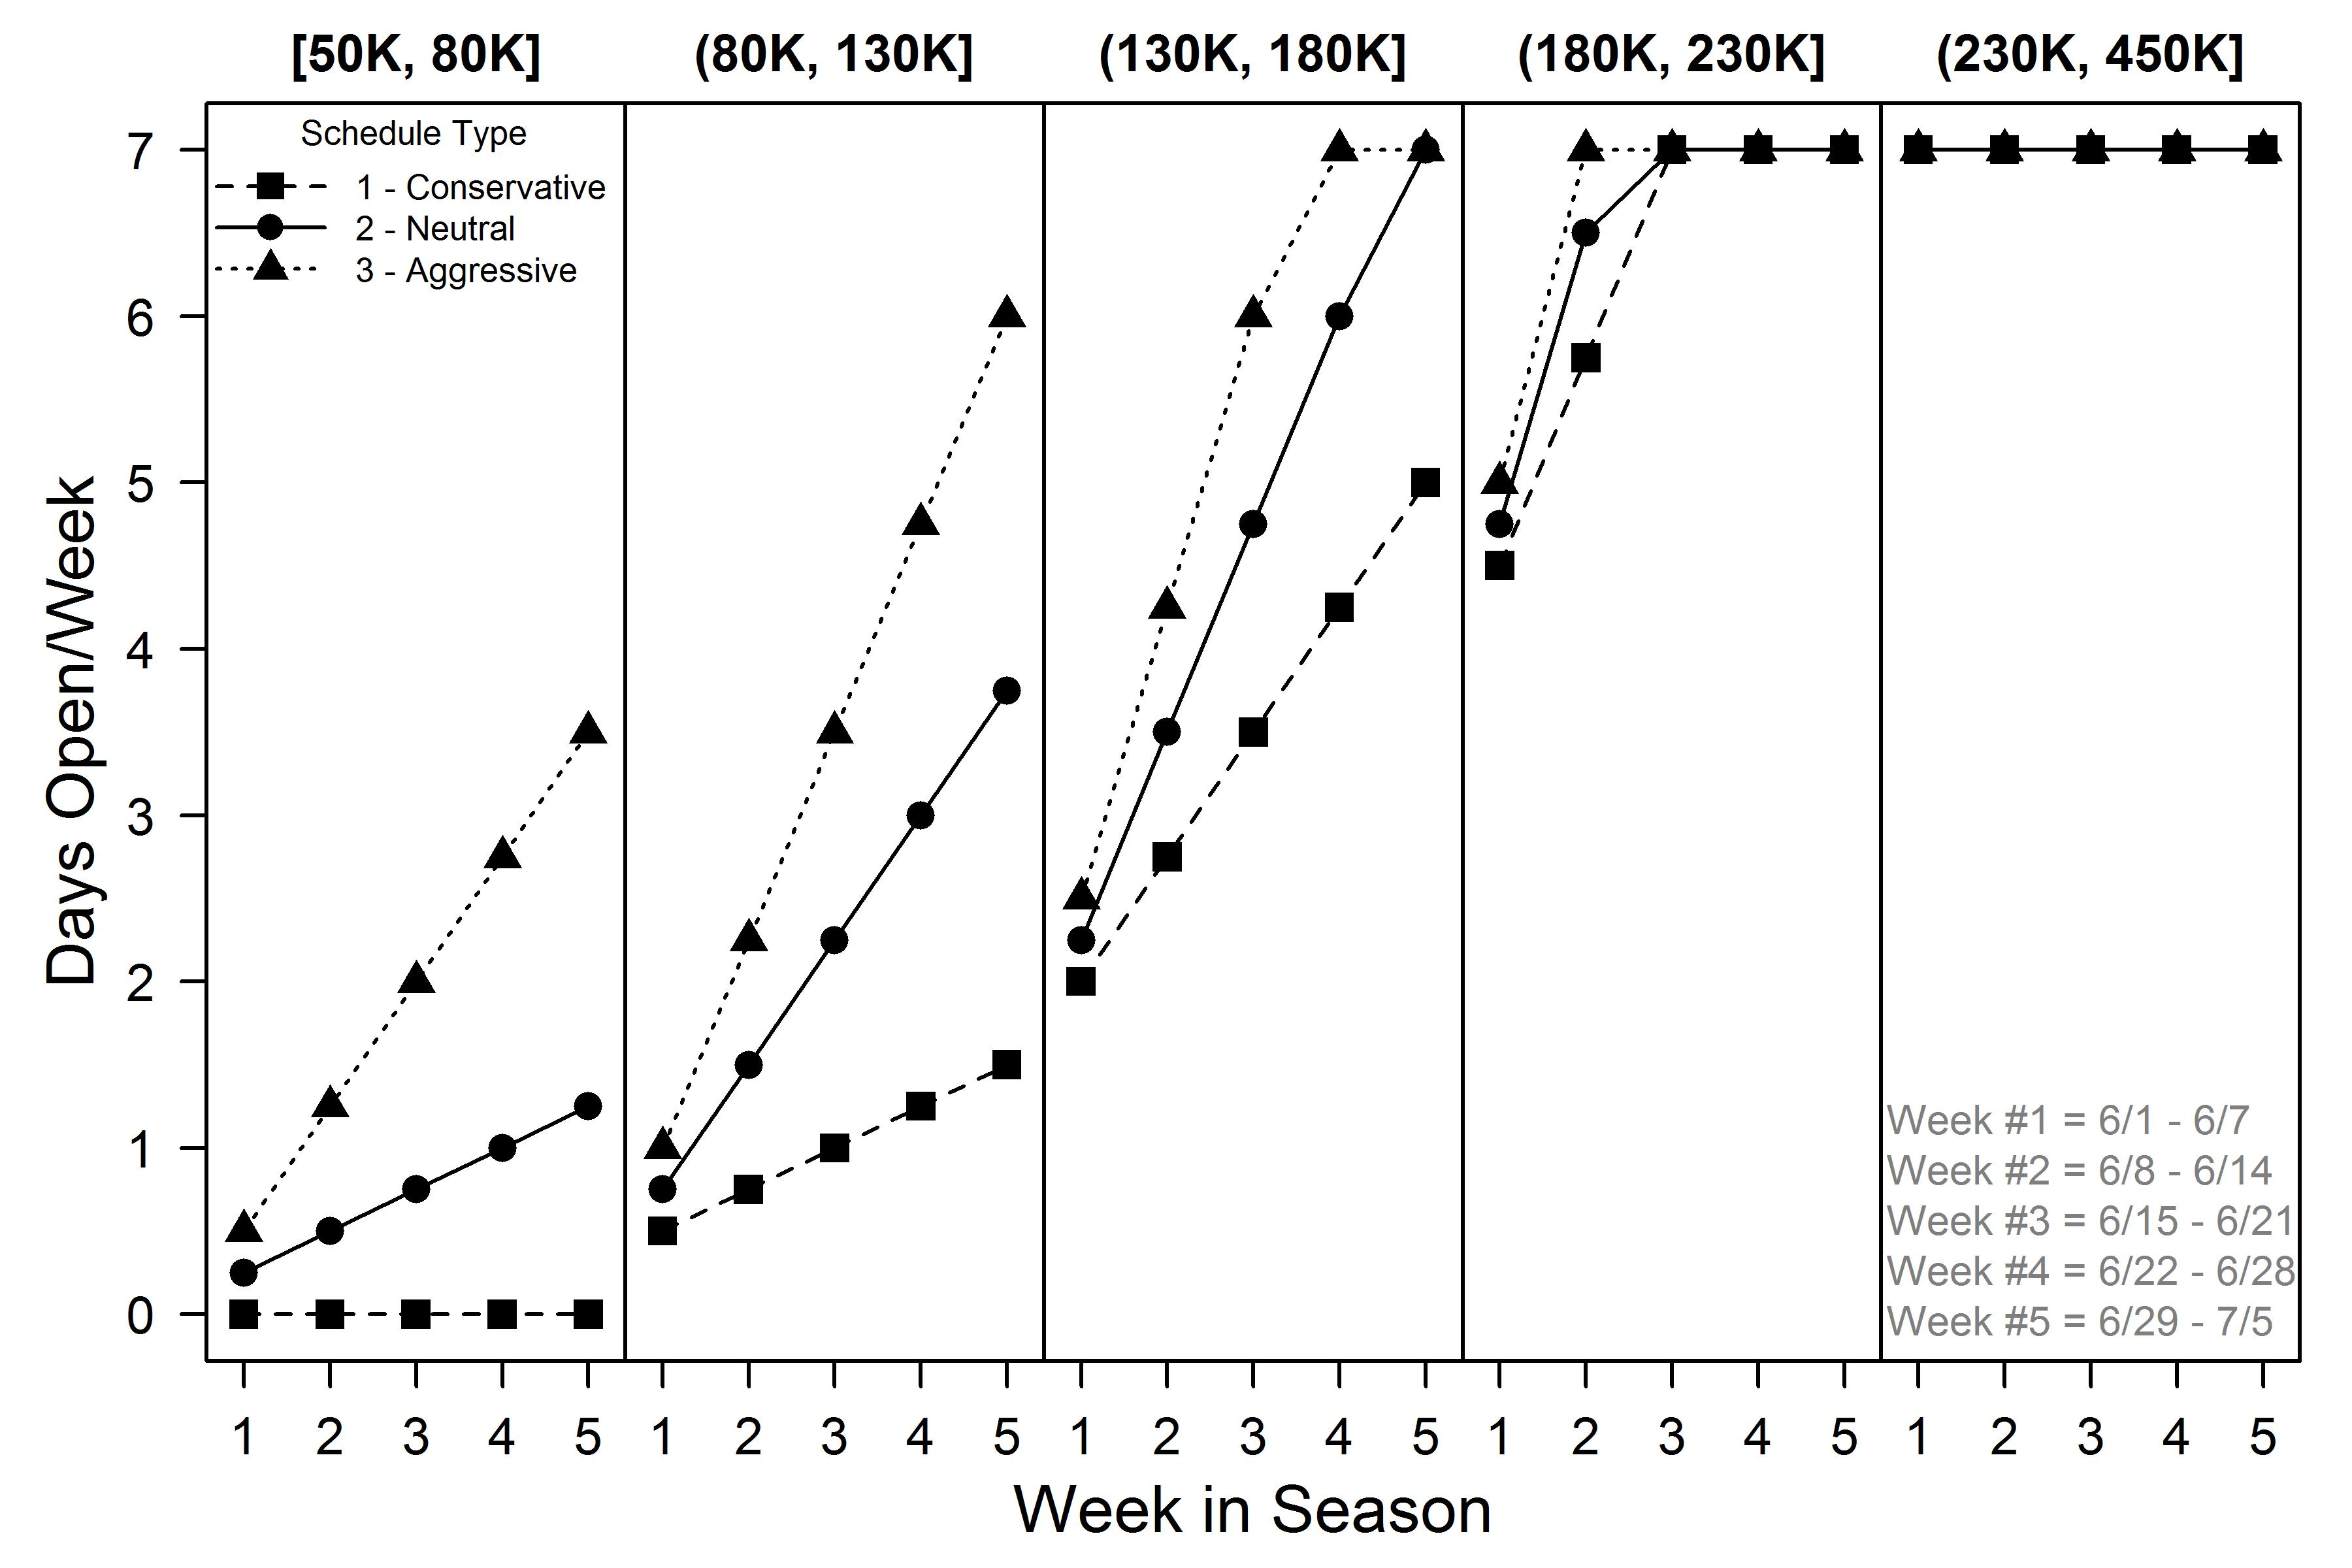
\includegraphics{img/Ch3/Schedules.png}
  \caption{Representation of the harvest control rule in assessed Strategies \#2 and \#3. The number of days the fishery is to be opened per week is a function of the pre-season forecast, as shown by each of the five panels. The three lines in each panel represent the different substrategies of Strategy \#2 or schedule types for Strategy \#3. In Strategy \#3, the manager would select to be conservative, neutral, or aggressive based on the percentile of recently-observed species ratios, as indicated in Table \ref{tab:ms3-ratio-table}. In other words, the manager using Strategy \#3 could adapt fishing schedules to in-season conditions, where as the \#2 manager could not.}
  \label{fig:ms2-schedules}
\end{figure}

\clearpage

\begin{figure}
  \centering
  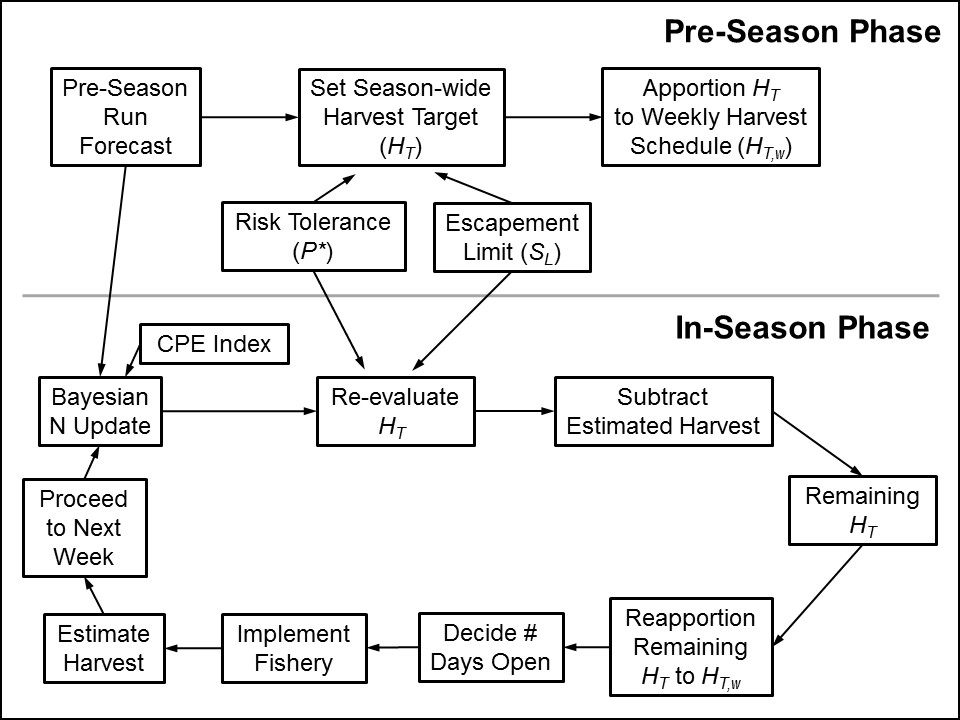
\includegraphics{img/Ch3/ms4-flow-diag.jpg}
  \caption{Depiction of the use of information to guide decision-making in assessed Strategy \#4, partitioned into pre-season and in-season phases. All actions are taken with regards to Chinook salmon. \textbf{Pre-season actions} occur only once per season, and involve producing a pre-season forecast (with error) and using it to set a season-wide harvest target ($H_T$) based on ($a$) the probability distribution representing uncertainty in the pre-season forecast, ($b$) a limit point that escapement cannot fall below ($S_L$), and ($c$) the maximal acceptable probability for seeing the outcome $S < S_L$ ($P^*$). Targeted harvest by week ($H_{T,w}$) is initially set by apportioning the total amongst weeks according to a fixed schedule based on historical run timing data. \textbf{In-season actions} are represented by a weekly cycle that involves updating perceptions of abundance and adapting the season-wide harvest target $H_T$ as appropriate to ensure the current posterior probability of attaining at least $S_L$ given $H_T$ still conforms with $P^*$, and the remaining allowable harvest for the season is obtained \textit{via} subtracting cumulative estimated harvest already taken. Remaining harvest is then apportioned to the remaining weeks, and based on the value of $H_{T,w}$, the fishery will be opened for between 0 and 7 days for the week according to the harvest tables displayed in Figure \ref{fig:ms4-schedules}. Harvest outcomes are monitored such that a weekly harvest estimate is available for use in the next week, which begins with obtaining a new posterior understanding of total run abundance.}
  \label{fig:ms4-flow-diag}
\end{figure}

\clearpage

\begin{figure}
  \centering
  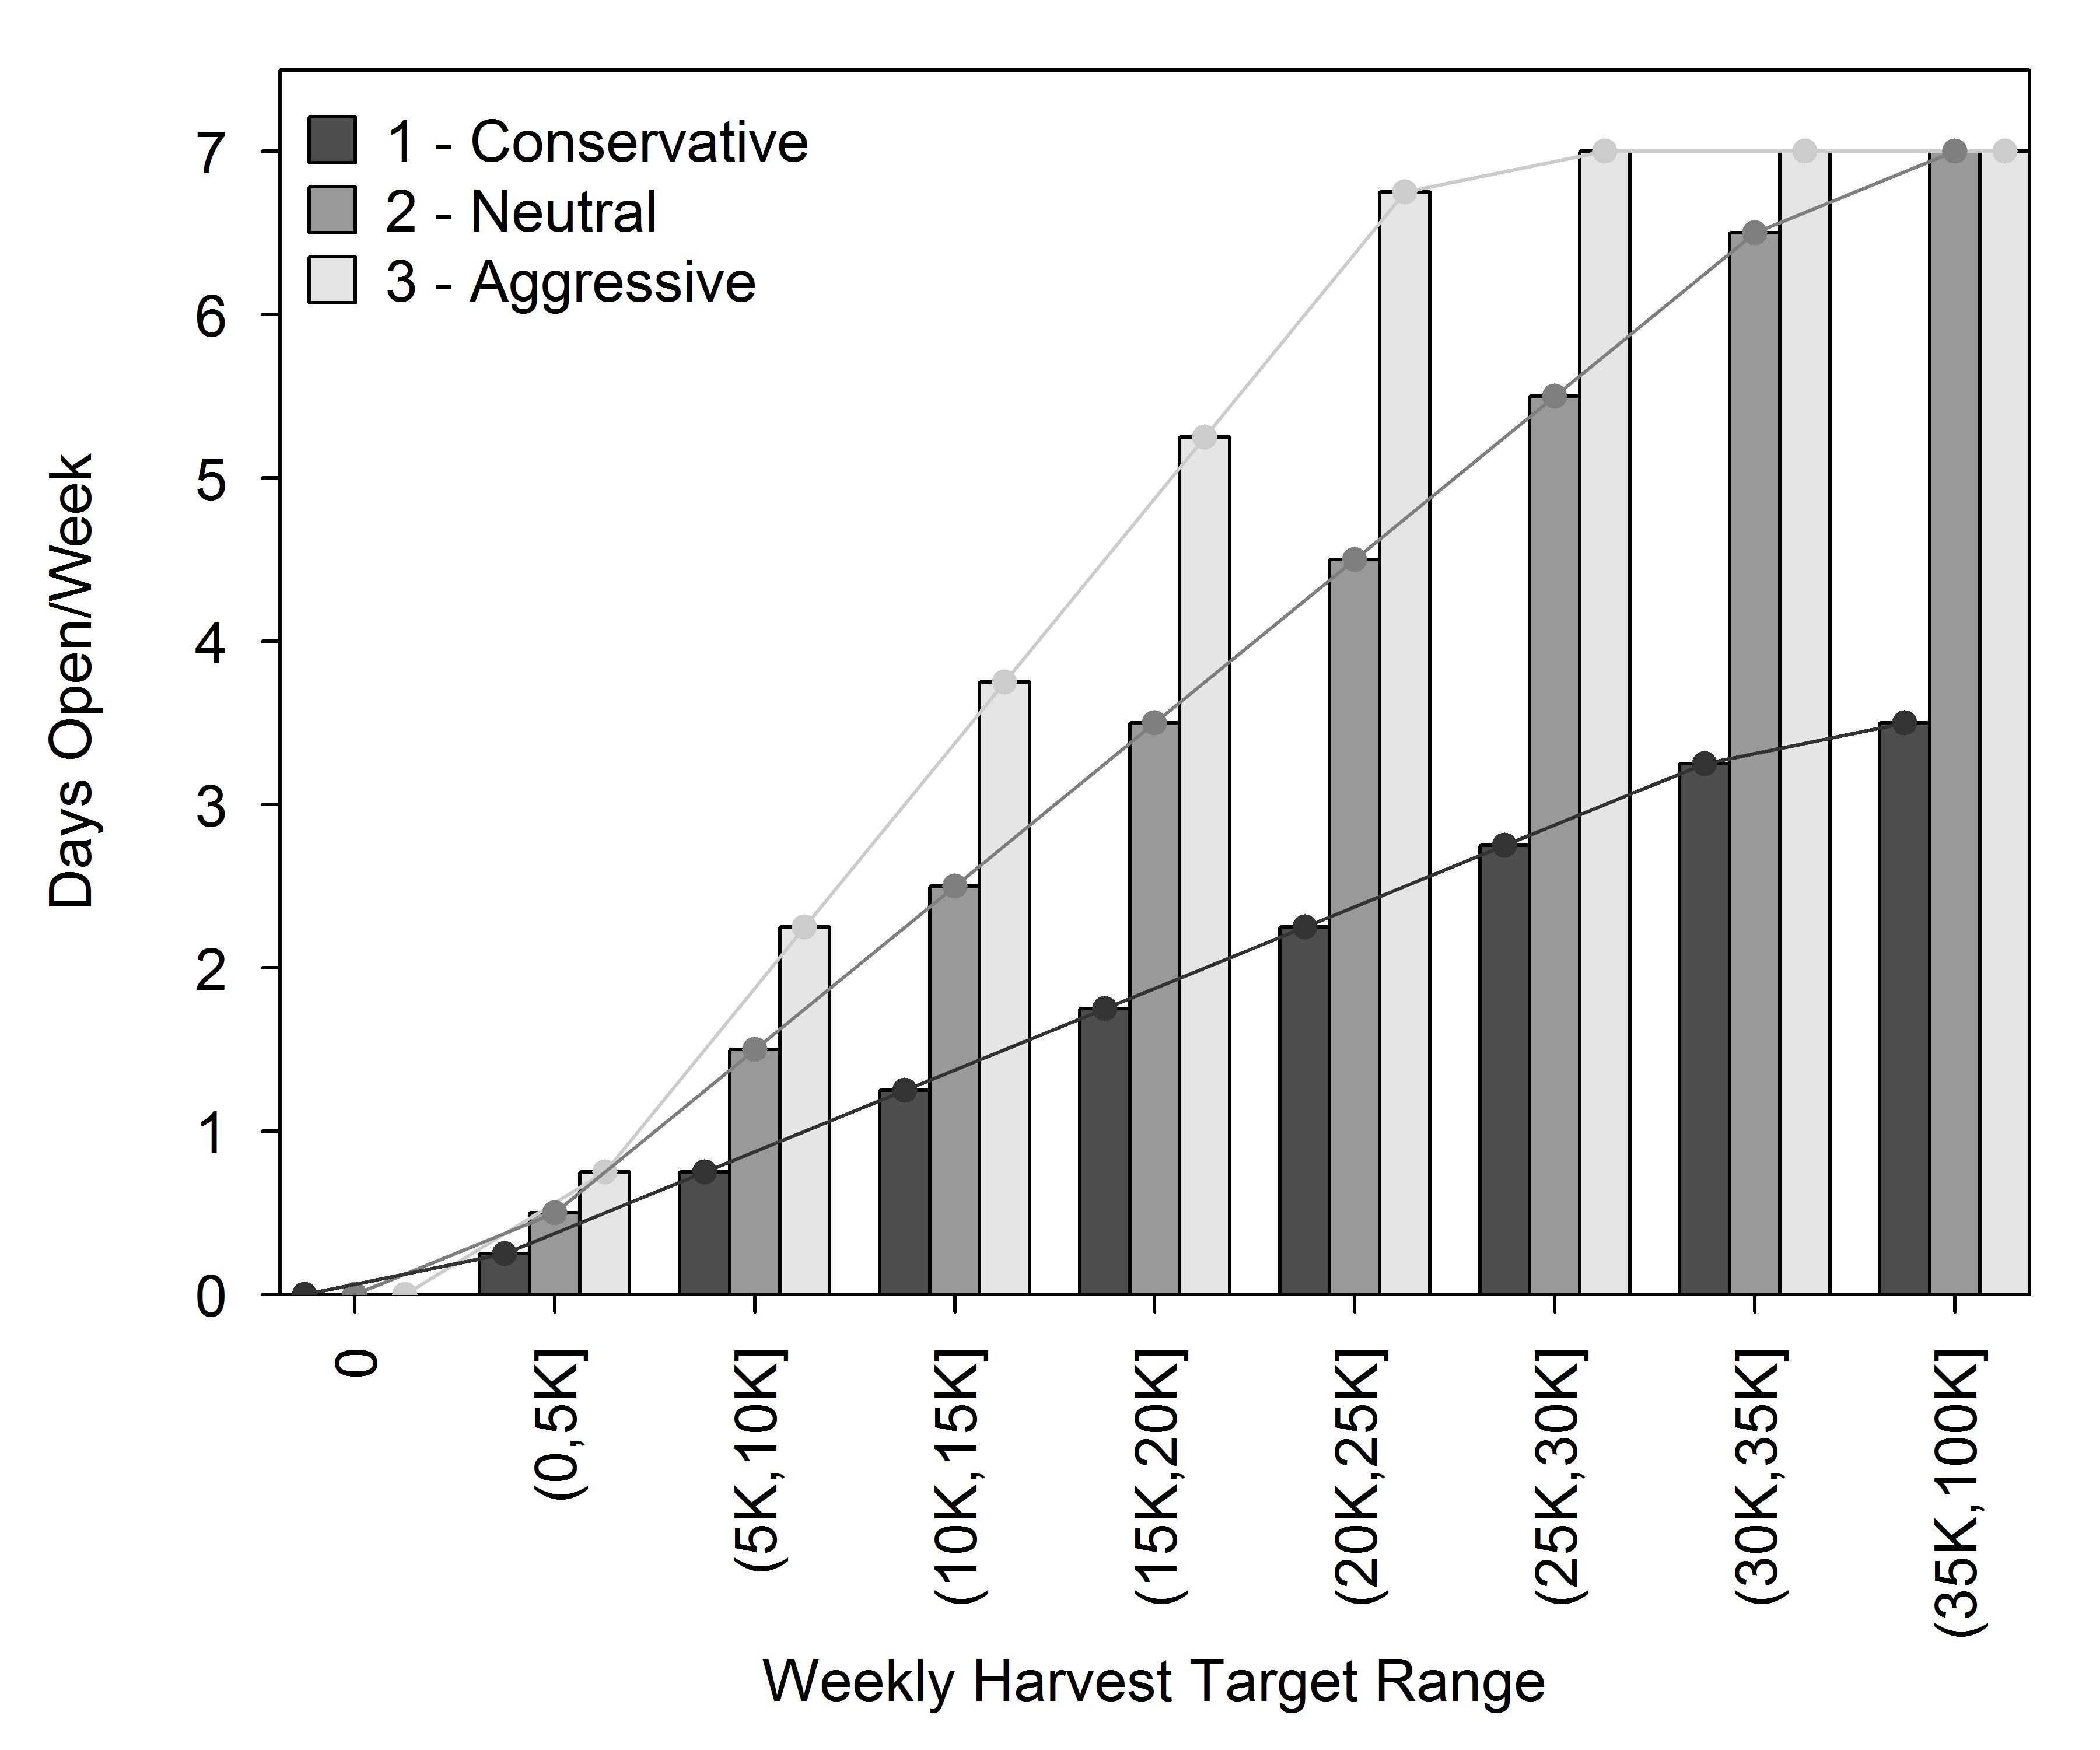
\includegraphics{img/Ch3/MS4_Schedules.jpg}
  \caption{Representation of the ``harvest tables'' used in assessed Strategy \#4. Based on how many fish are targeted each particular week ($H_{T,w}$), the manager would select the number of days to open the fishery. The process to obtain $H_{T,w}$ was rather involved, requiring pre-season forecasts, in-season abundance index data, and in-season harvest data to inform its value, as shown in Figure \ref{fig:ms4-flow-diag}.}
  \label{fig:ms4-schedules}
\end{figure}

\clearpage

\begin{figure}
  \centering
  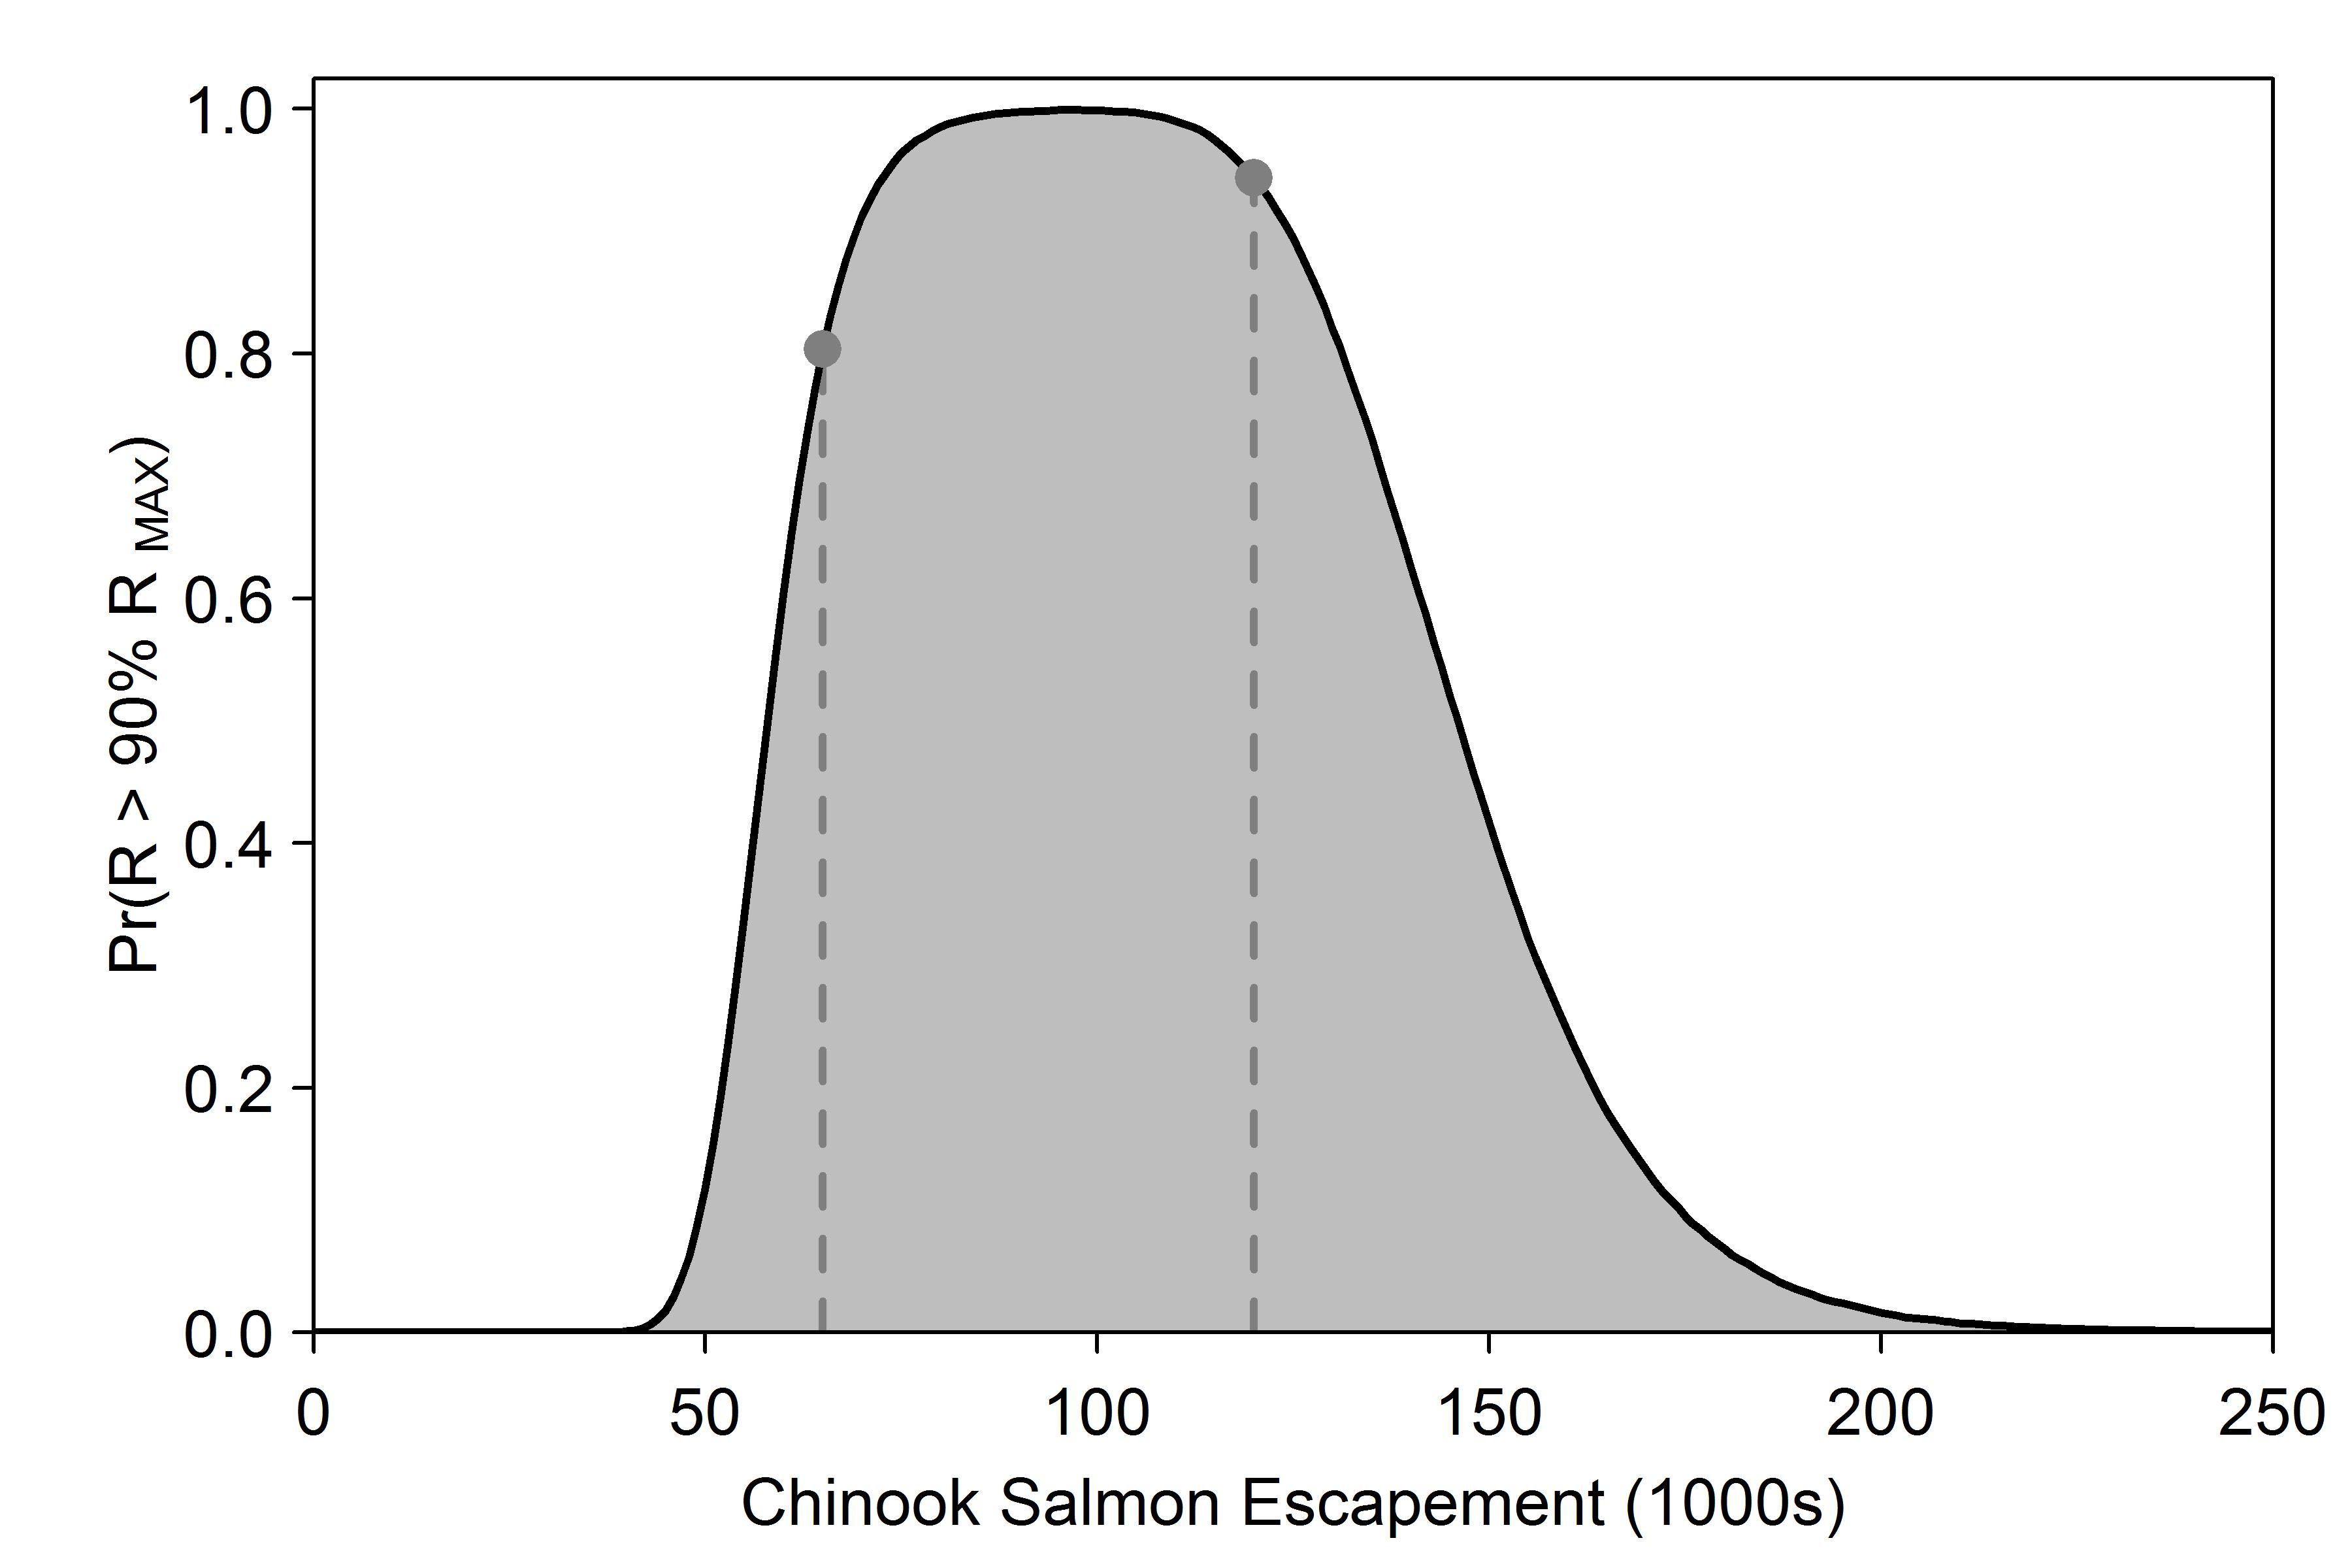
\includegraphics{img/Ch3/R-max-profile.jpg}
  \caption{Estimated probability profile for Kuskokwim River Chinook salmon used as the utility function for drainage-wide escapement in this analysis. The height of the curve represents the currently understood probability that expected recruitment produced by a given escapement level will exceed 90\% of $R_{\text{MAX}}$, and was obtained for the aggregate Chinook salmon stock using the Bayesian state-space estimation model presented in \cite{hamazaki-etal-2012} updated with abundance, harvest, and age composition data through 2017. The vertical dashed lines are the endpoints of the current escapement goal range.}
  \label{fig:R-max-profile}
\end{figure}

\clearpage
\begin{figure}
  \centering
  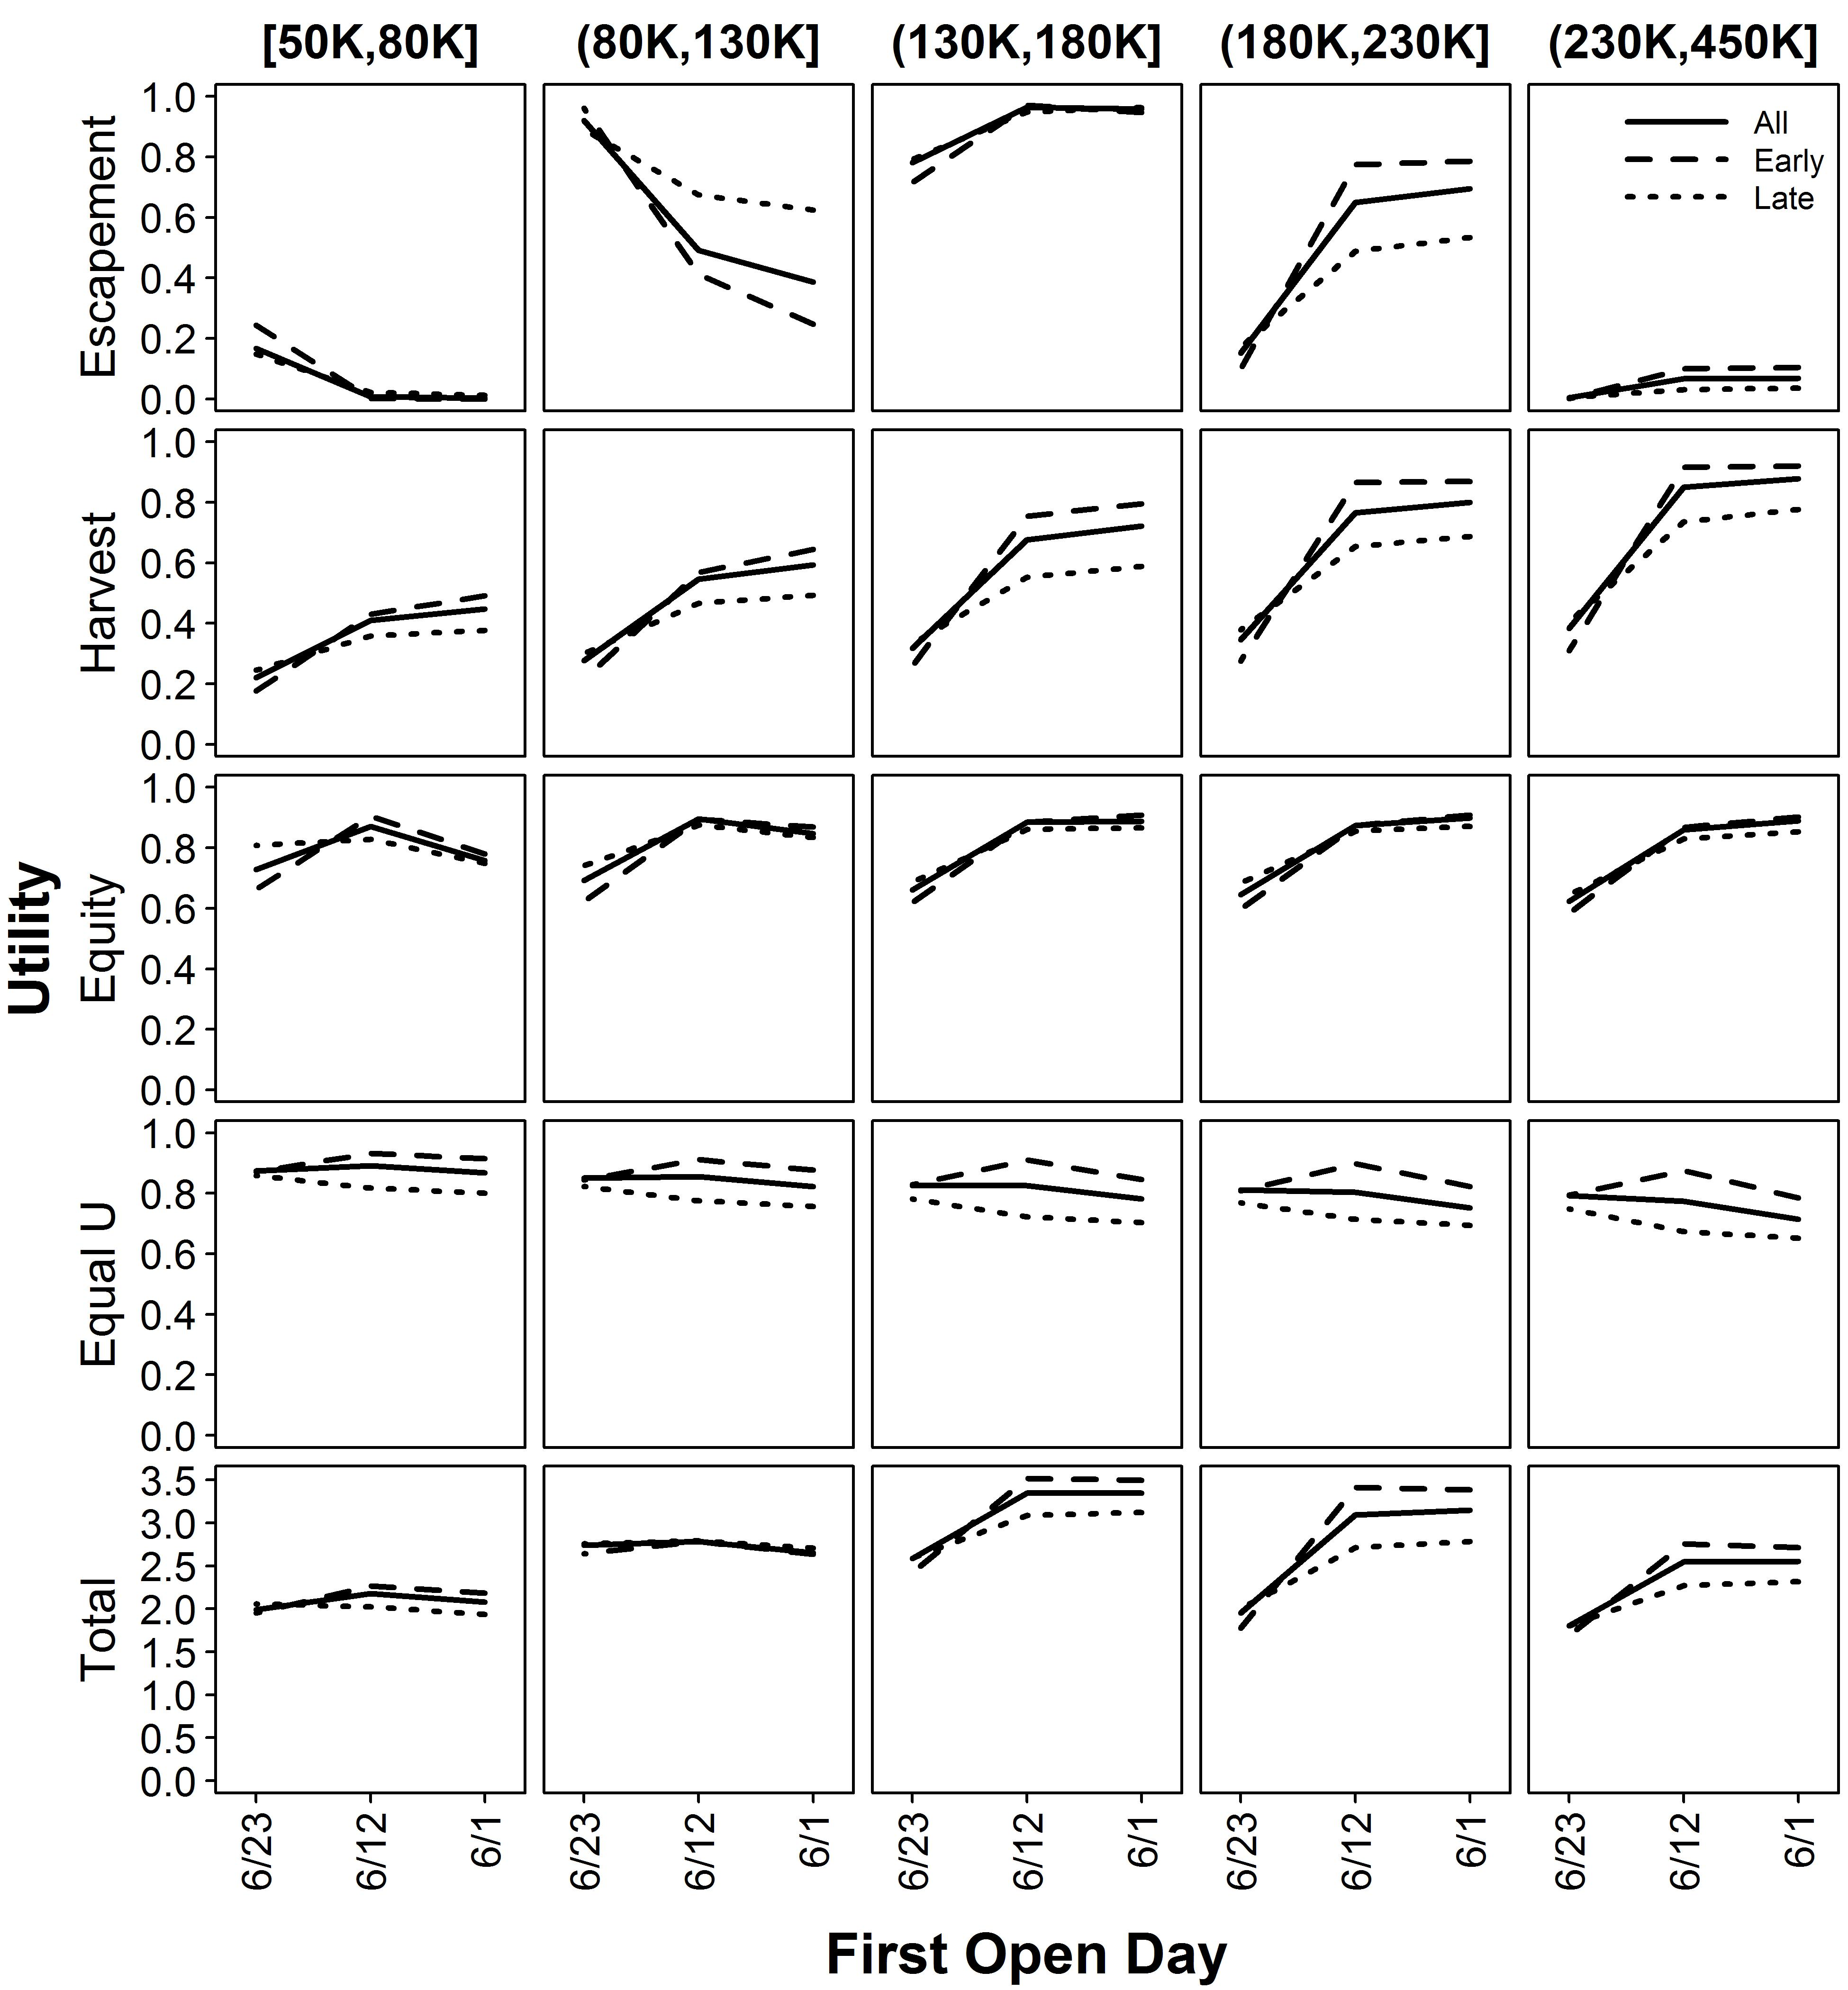
\includegraphics{img/Ch3/Values_1.jpg}
  \caption{Detailed performance of assessed Strategy \#1. Values of the utility functions (rows) separated by run size category (horizontal panels), run timing category (line type), and substrategy ($x$-axis, ordered from most conservative to aggressive). Substrategies of this policy differ in the date at which the fishery is opened completely. The form of each utility function is described in Section \ref{utility-funcs}, and the total metric shown uses the default weighting scheme (all objective weights equal to 1).}
  \label{fig:ms1-utilities}
\end{figure}

\clearpage
\begin{figure}
  \centering
  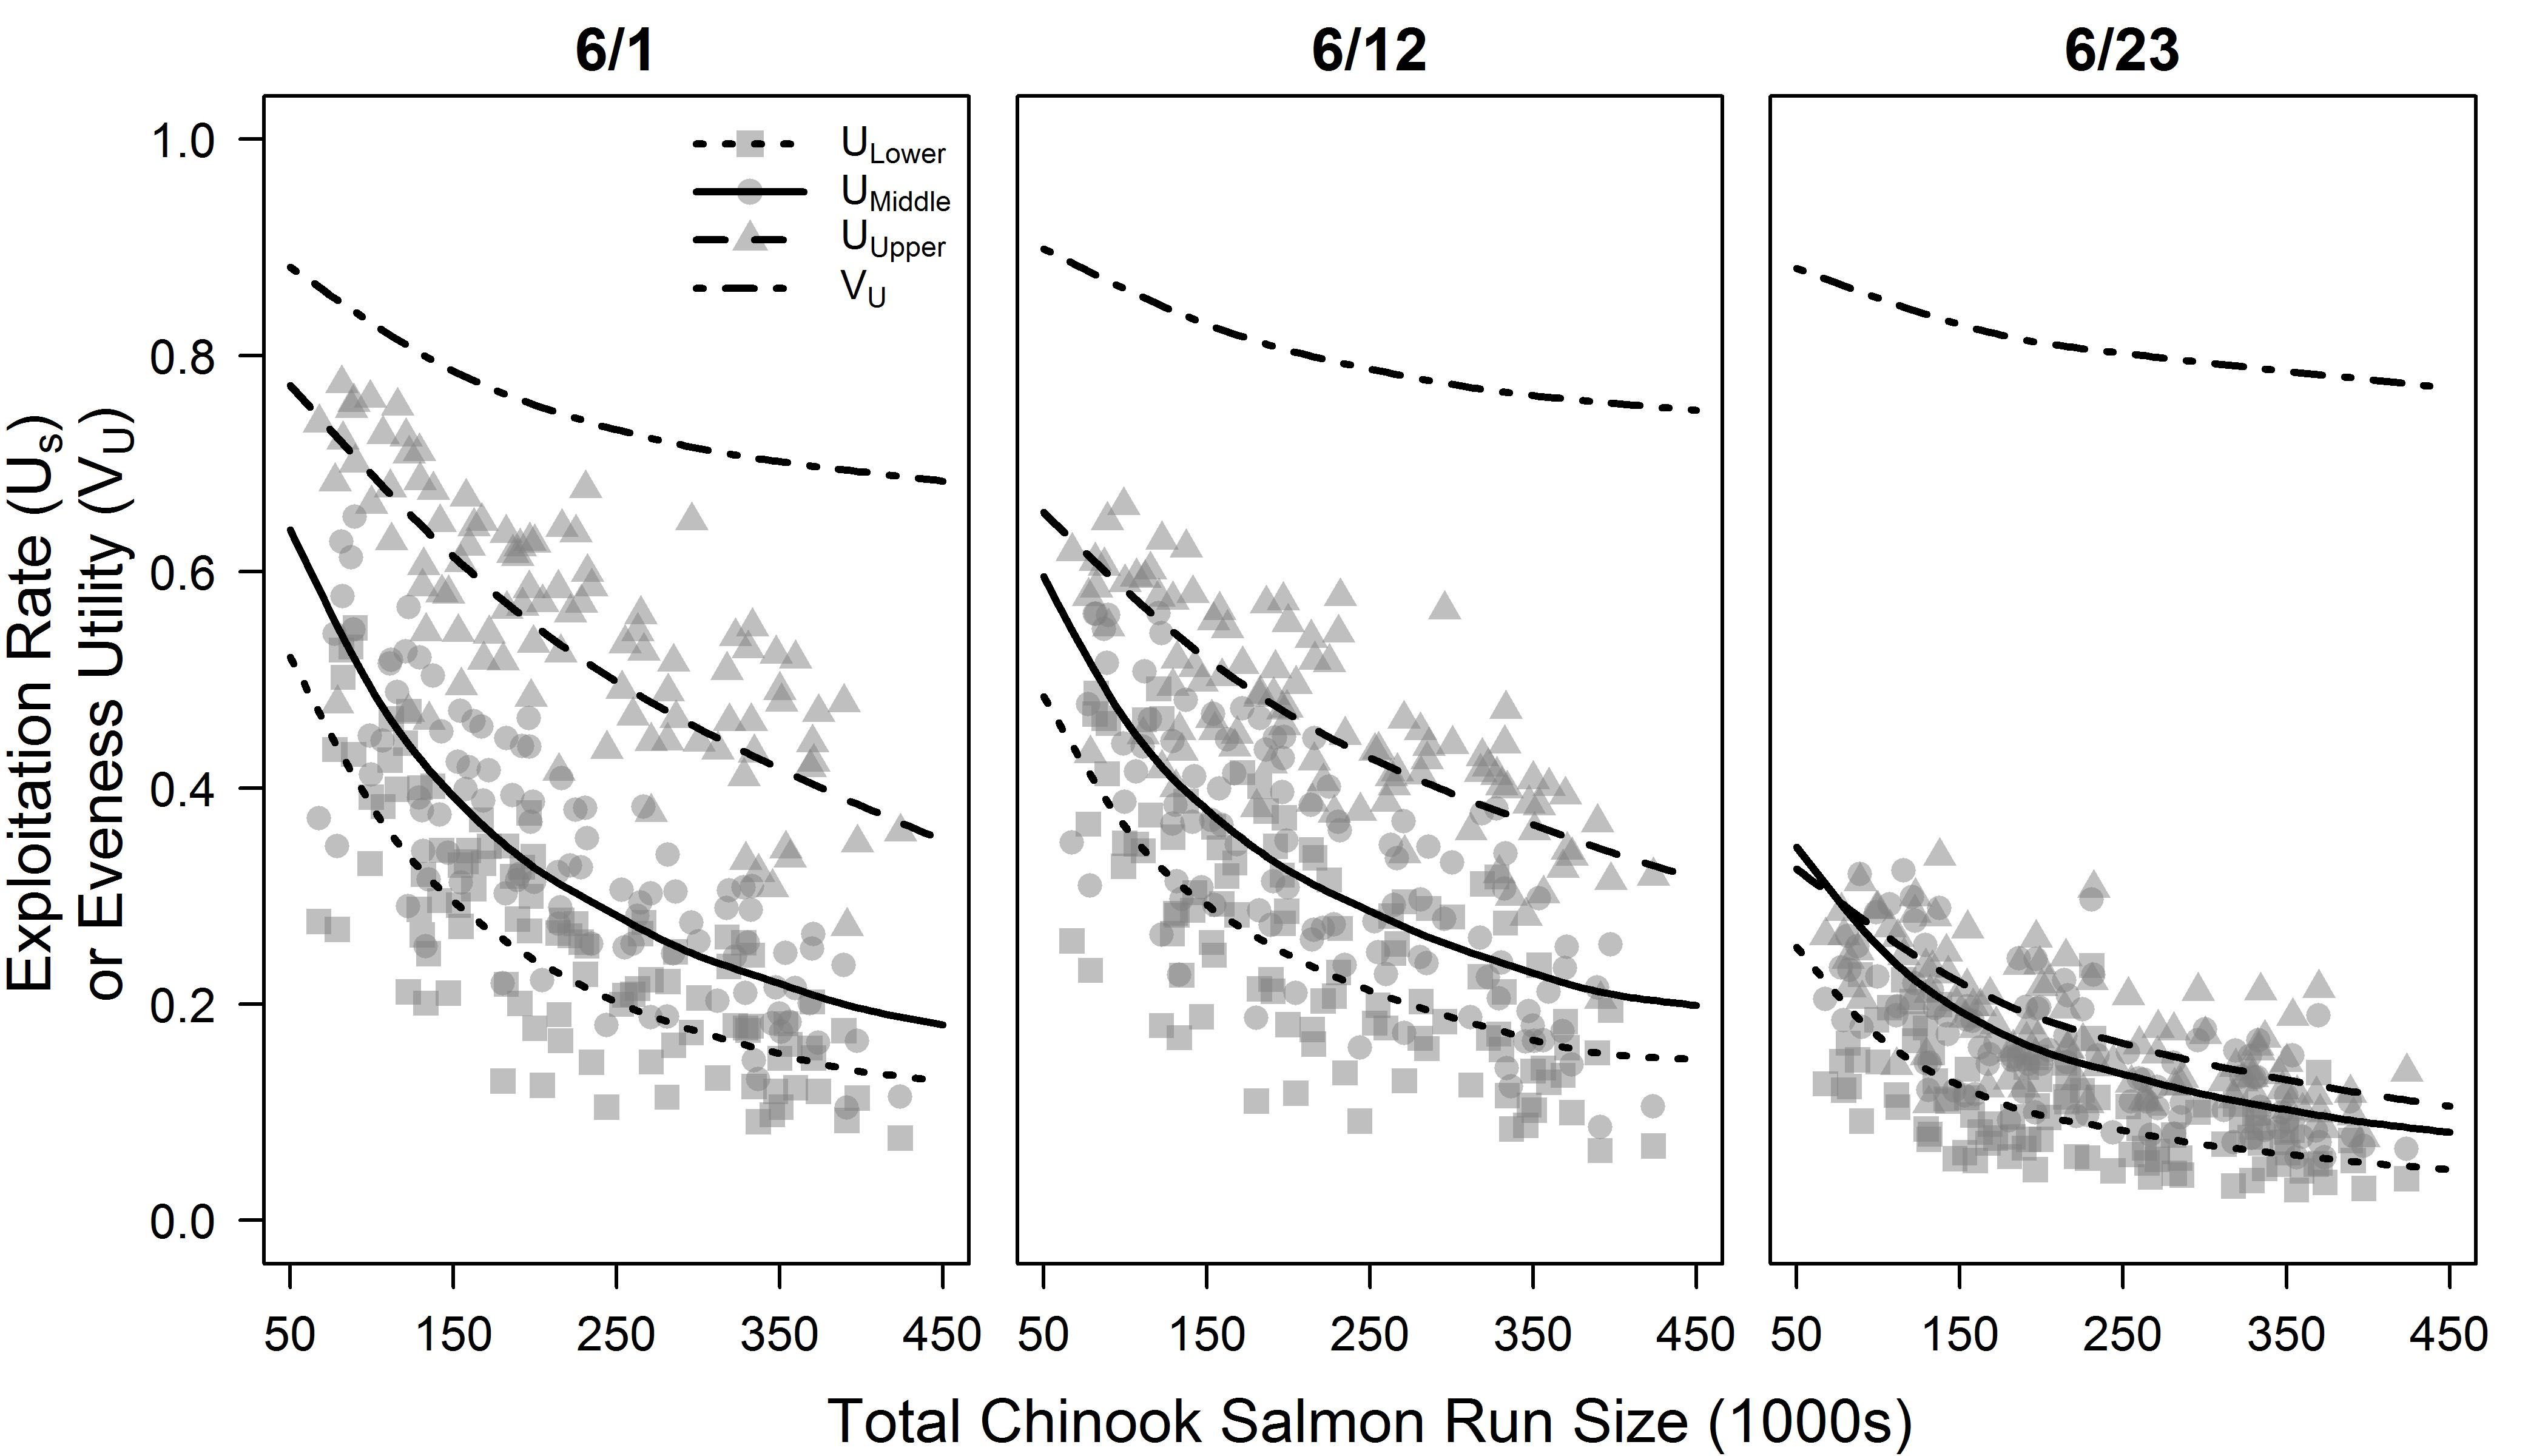
\includegraphics{img/Ch3/U-v-N.jpg}
  \caption{Chinook salmon substock-specific exploitation rates as a function of run size, separated by different substrategies (i.e., opening dates) of assessed Strategy \#1. Lines are fitted generalized additive models. The line denoted by $V_U$ represents the model fitted to the utility metric as defined by the modified Schutz coefficient used.}
  \label{fig:U-v-N}
\end{figure}

\clearpage
\begin{figure}
  \centering
  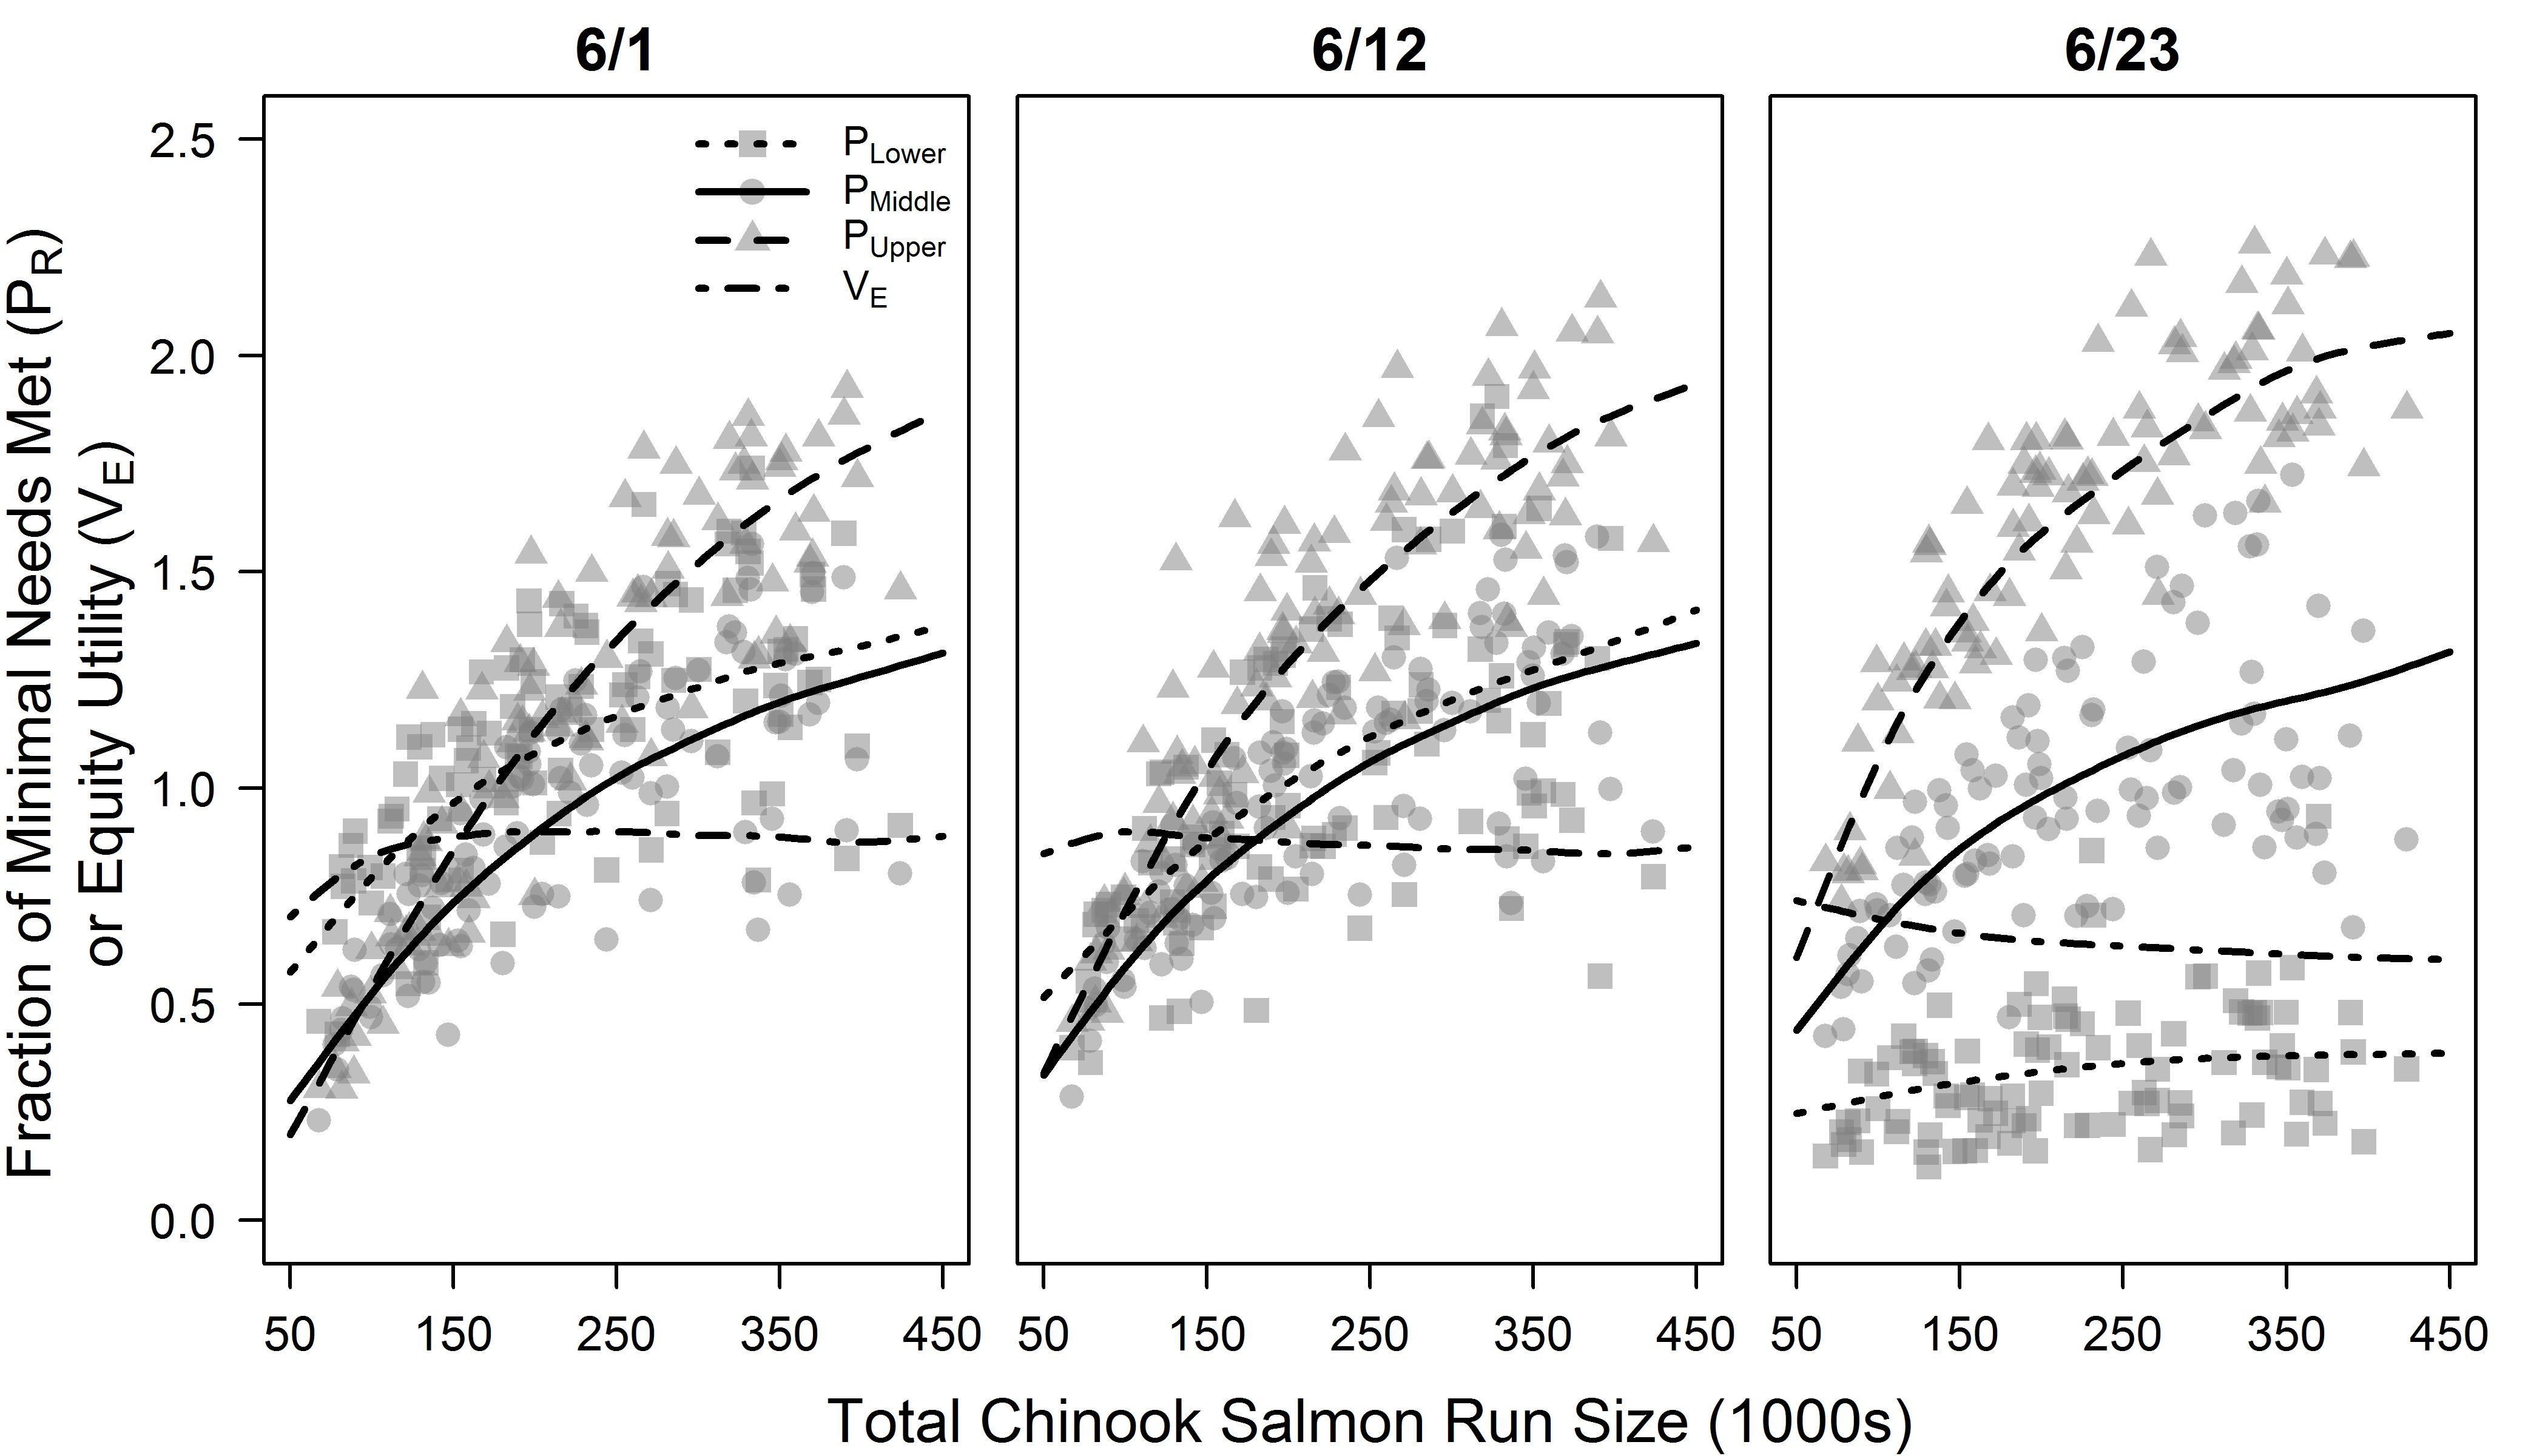
\includegraphics{img/Ch3/pNeed-v-N.jpg}
  \caption{The fraction of minimal Chinook salmon harvest attained by villages in the lower, middle, and upper regions of the simulated Kuskokwim River as a function of run size, separated by different substrategies (i.e., opening dates) of assessed Strategy \#1. Lines are fitted generalized additive models. The line denoted by $V_E$ represents the model fitted to the utility metric as defined by the modified Schutz coefficient used.}
  \label{fig:pNeed-v-N}
\end{figure}

\clearpage
\begin{figure}
  \centering
  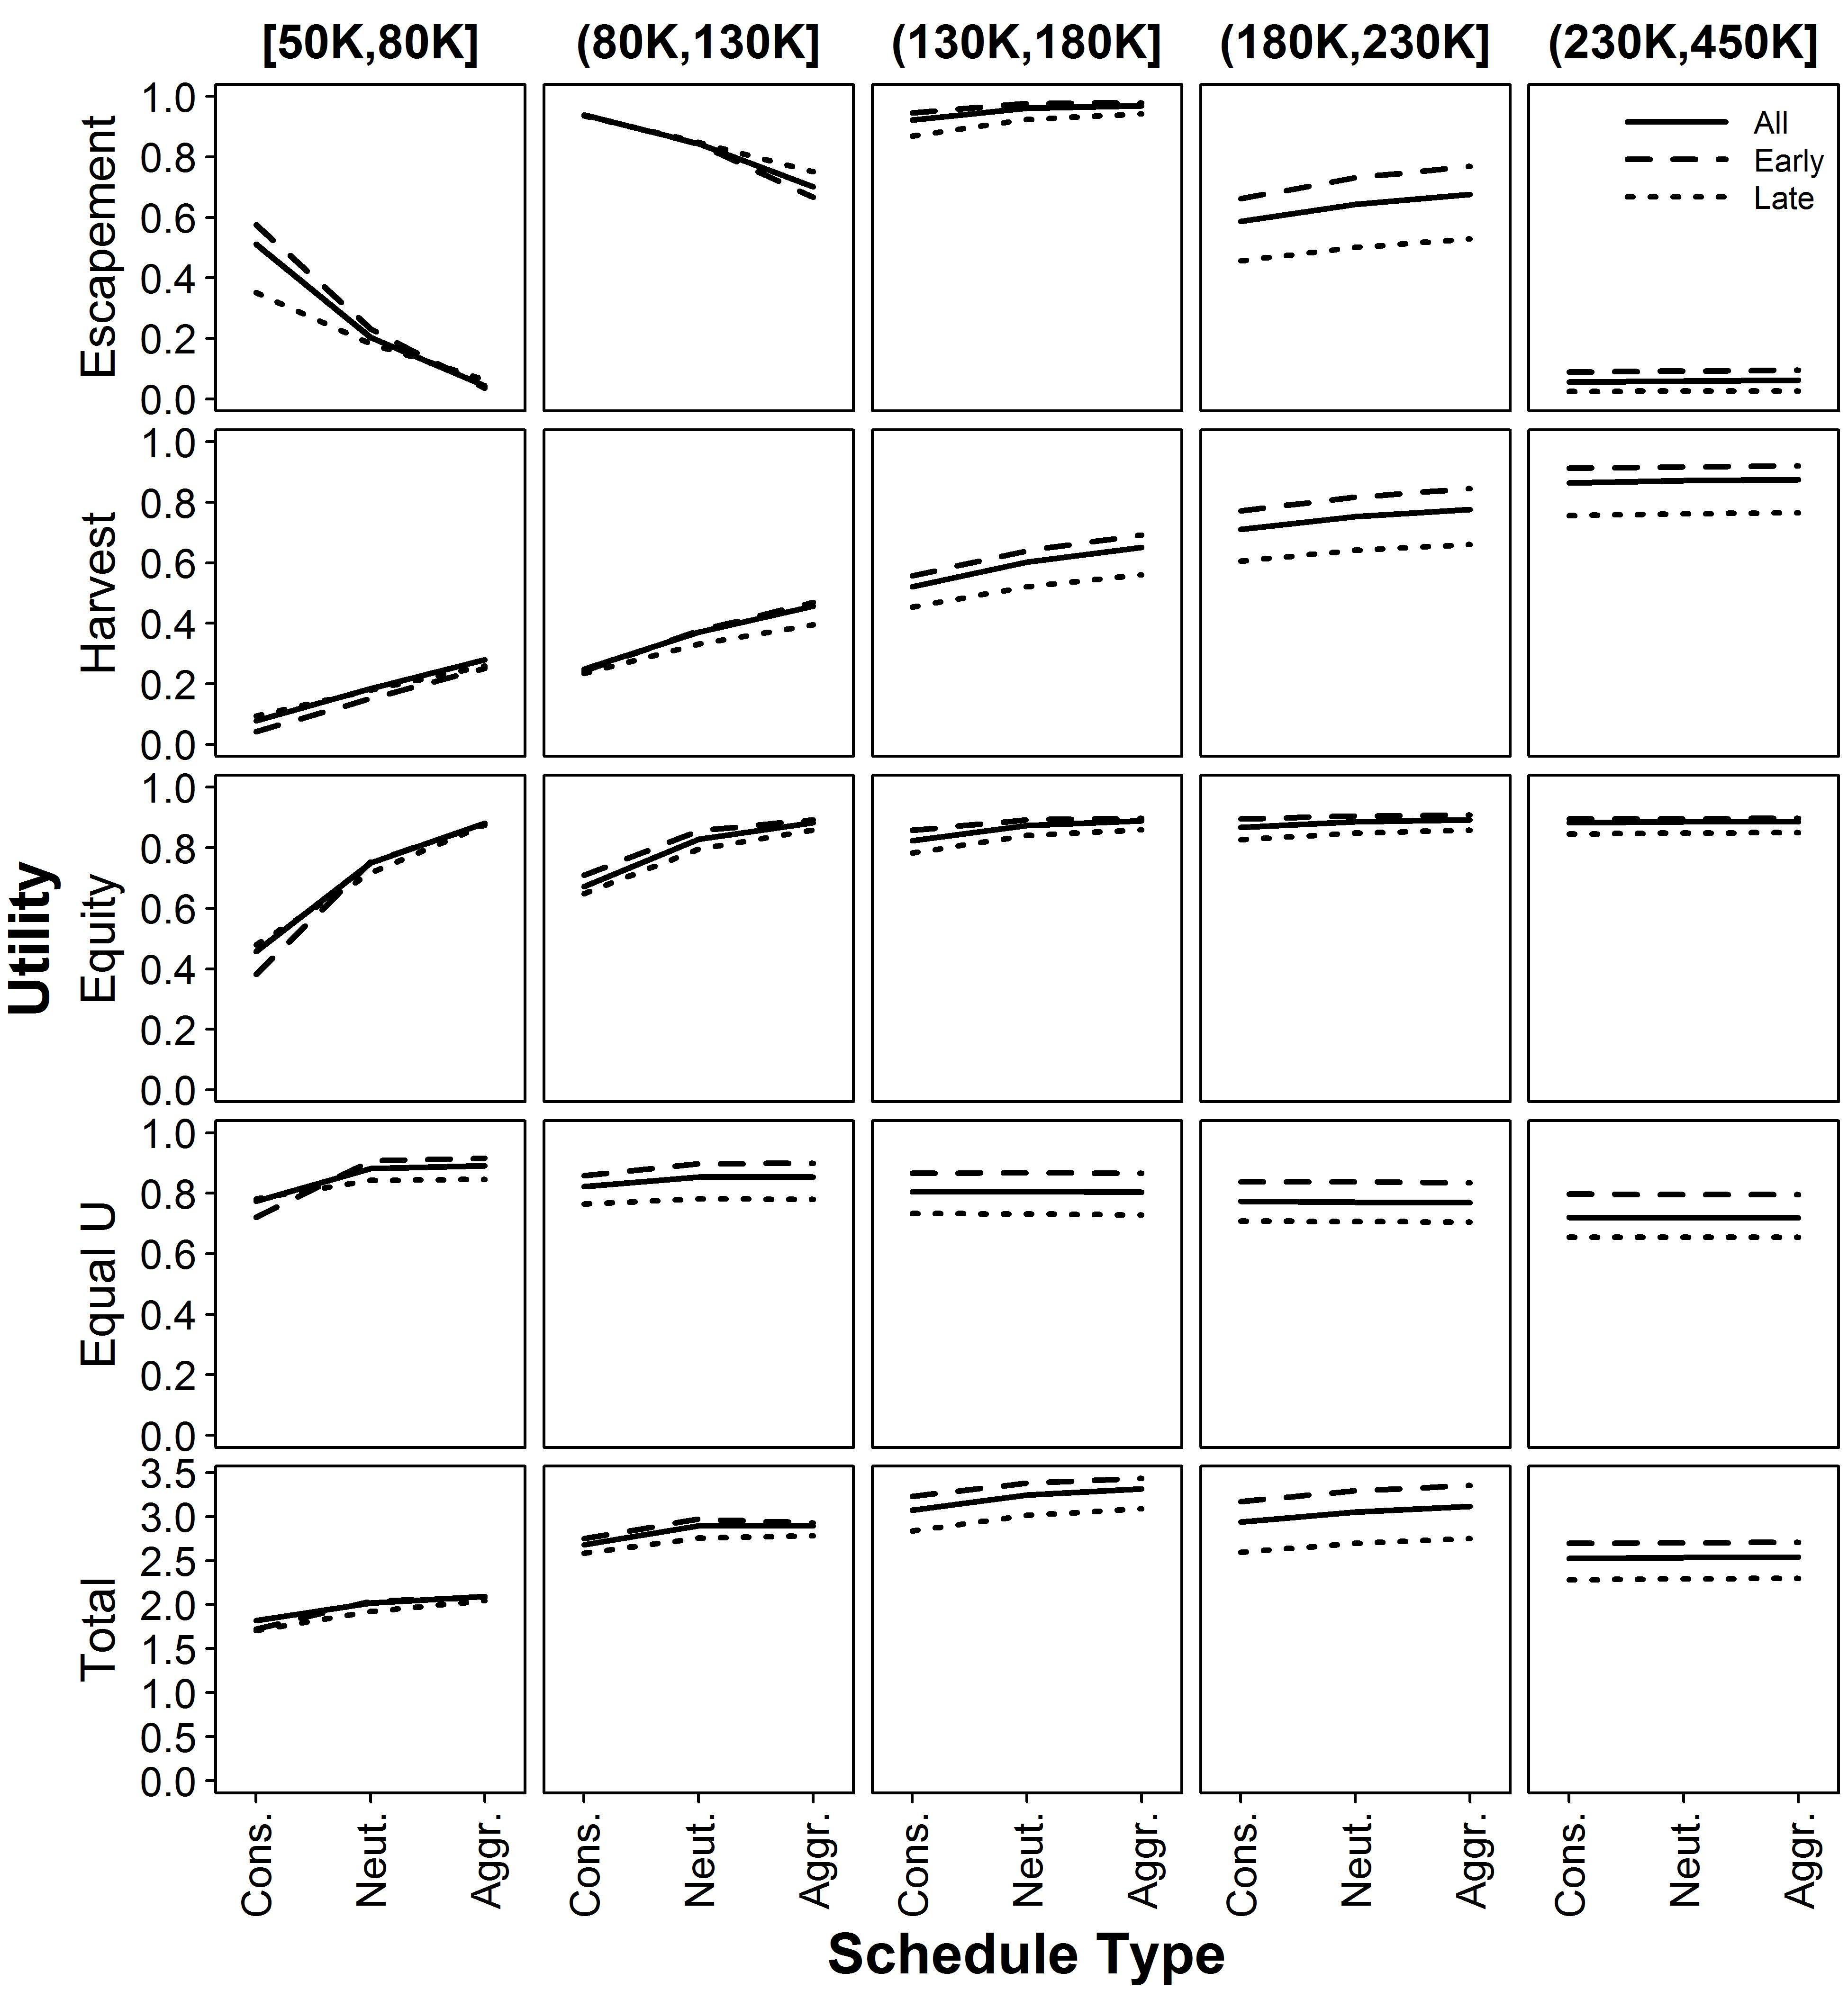
\includegraphics{img/Ch3/Values_2.jpg}
  \caption{Detailed performance of assessed Strategy \#2. The layout of panels in this figure is the same as in Figure \ref{fig:ms1-utilities}, only substrategies represent different schedules conditional on a pre-season run size forecast (schedules shown in Figure \ref{fig:ms2-schedules}).}
  \label{fig:ms2-utilities}
\end{figure}

\clearpage
\begin{figure}
  \centering
  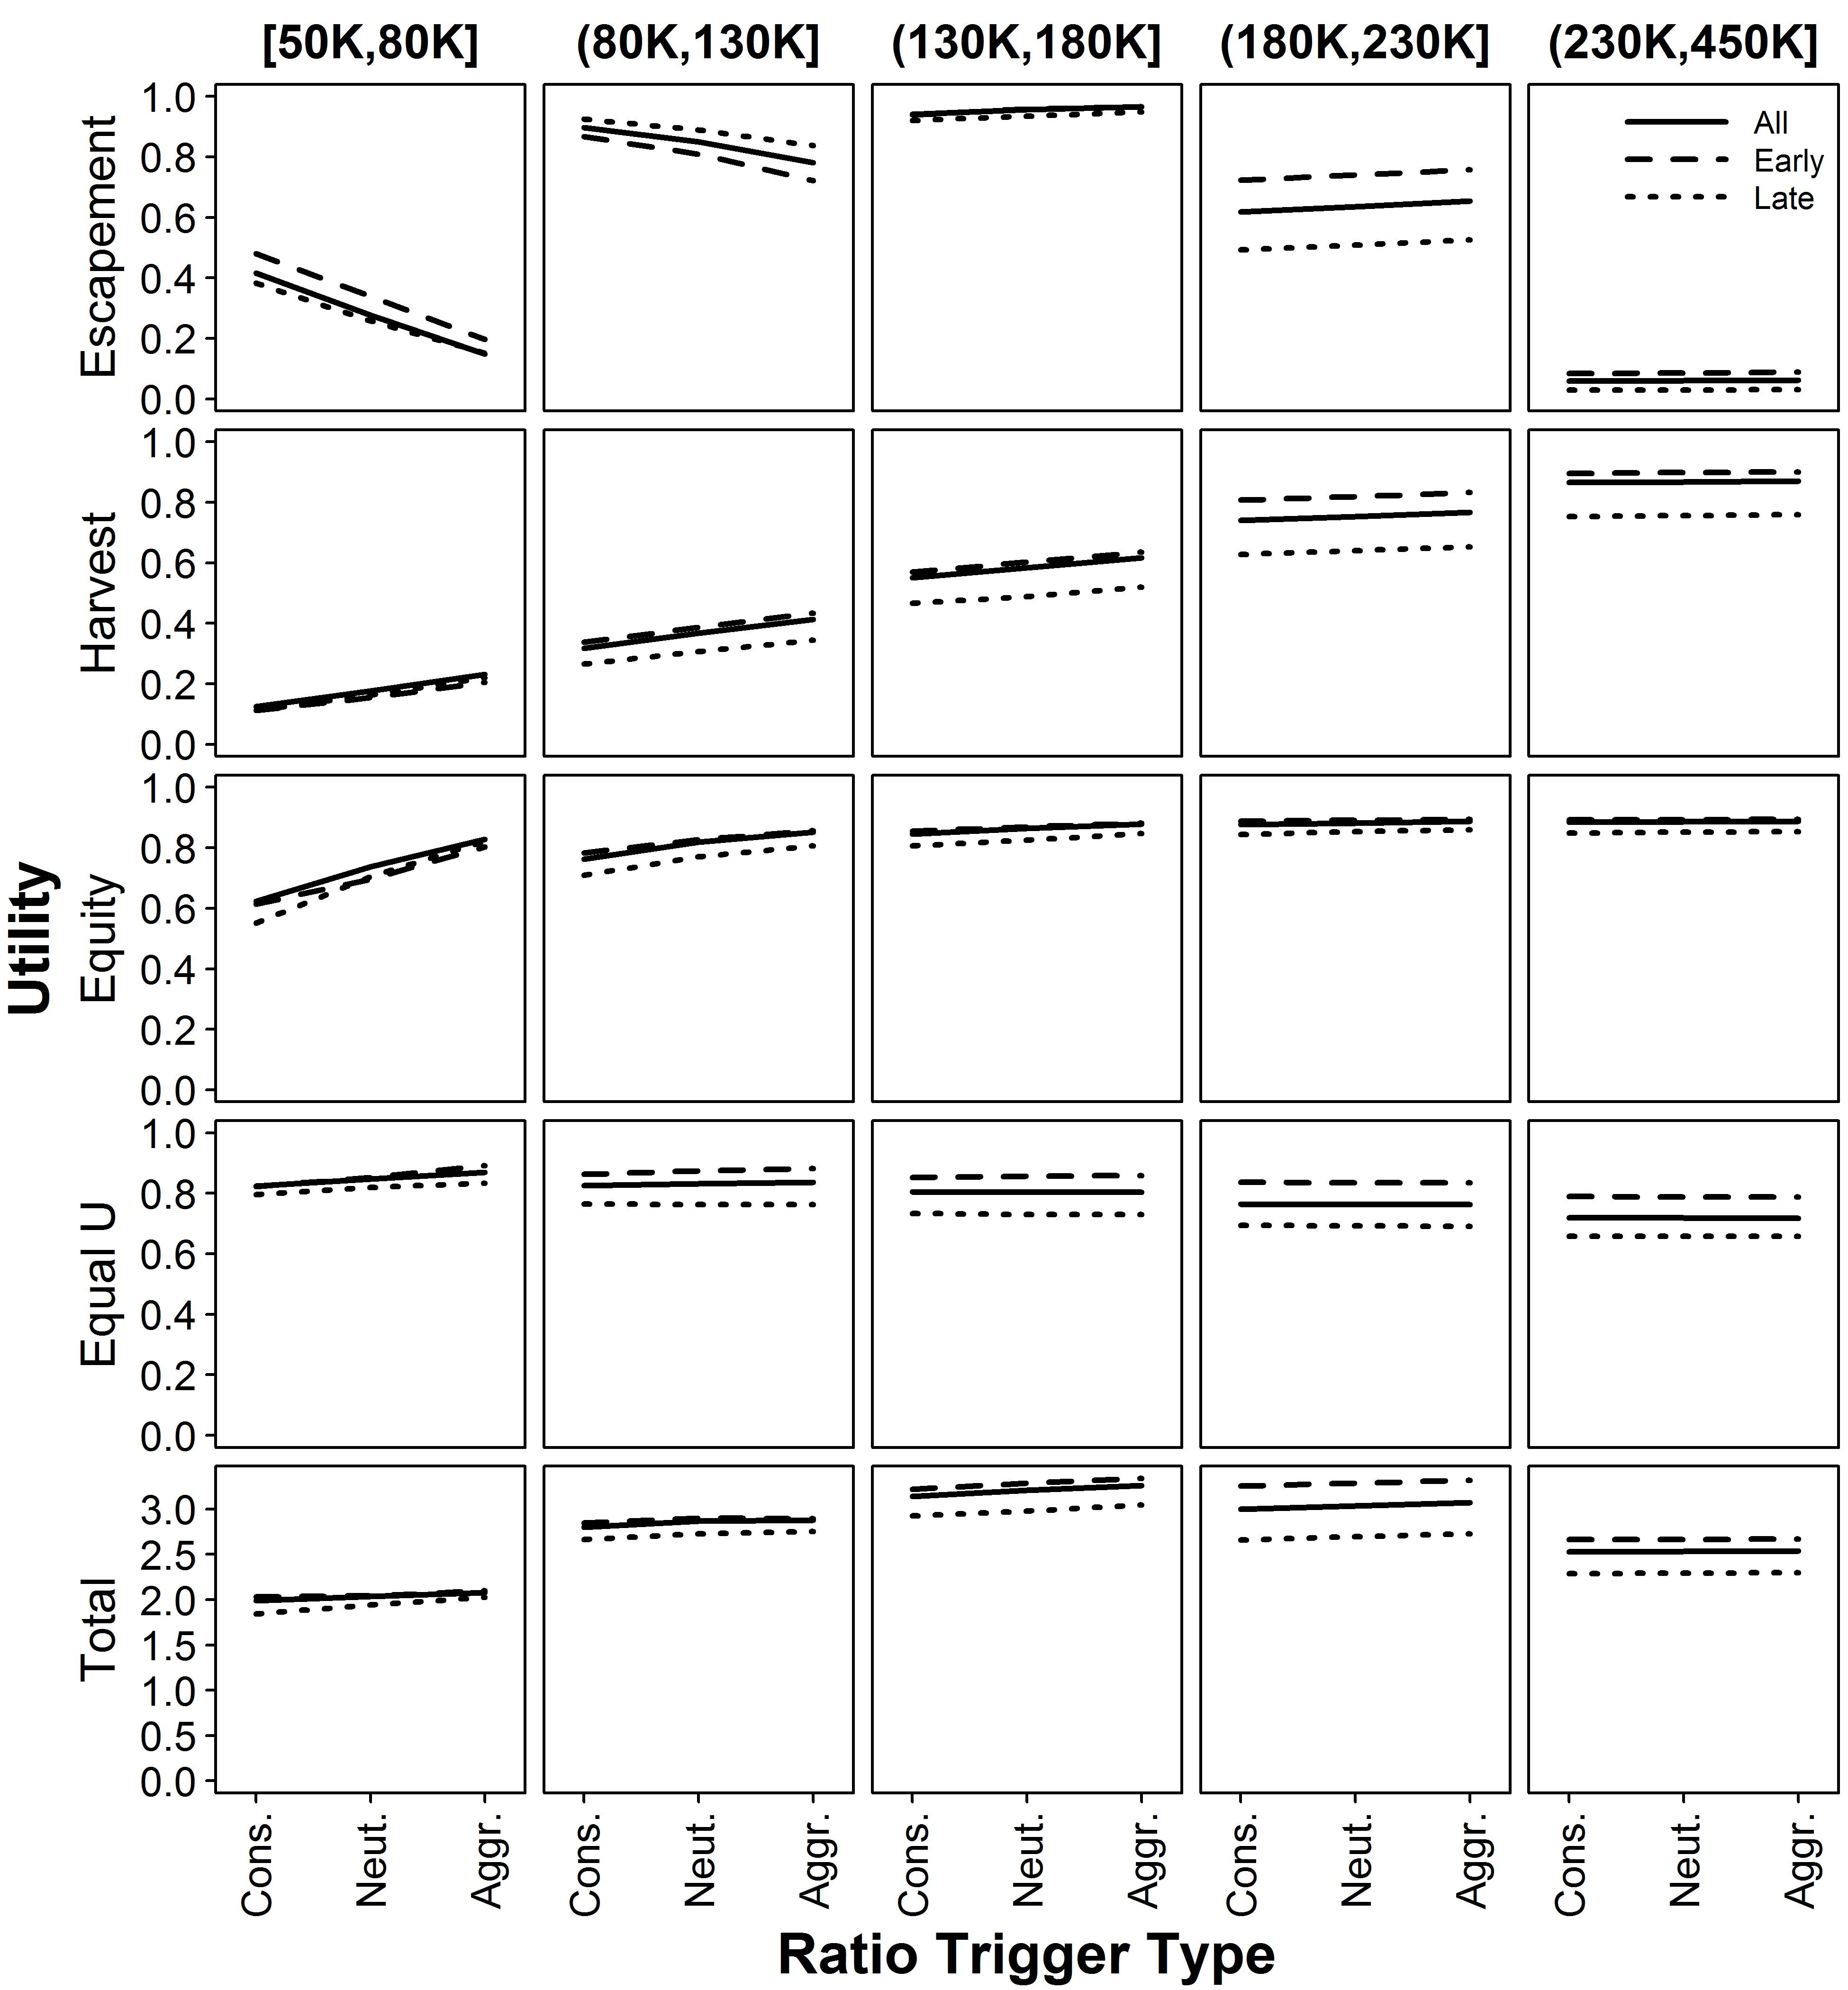
\includegraphics{img/Ch3/Values_3.jpg}
  \caption{Detailed performance of assessed Strategy \#3. The layout of panels in this figure is the same as in Figure \ref{fig:ms1-utilities}, only substrategies represent different species ratios cut-offs used to pick fishing schedules conditional on a pre-season run size forecast (schedules shown in Figure \ref{fig:ms2-schedules}, ratio thresholds shown in Table \ref{tab:ms3-ratio2-table}).}
  \label{fig:ms3-utilities}
\end{figure}

\clearpage
\begin{figure}
  \centering
  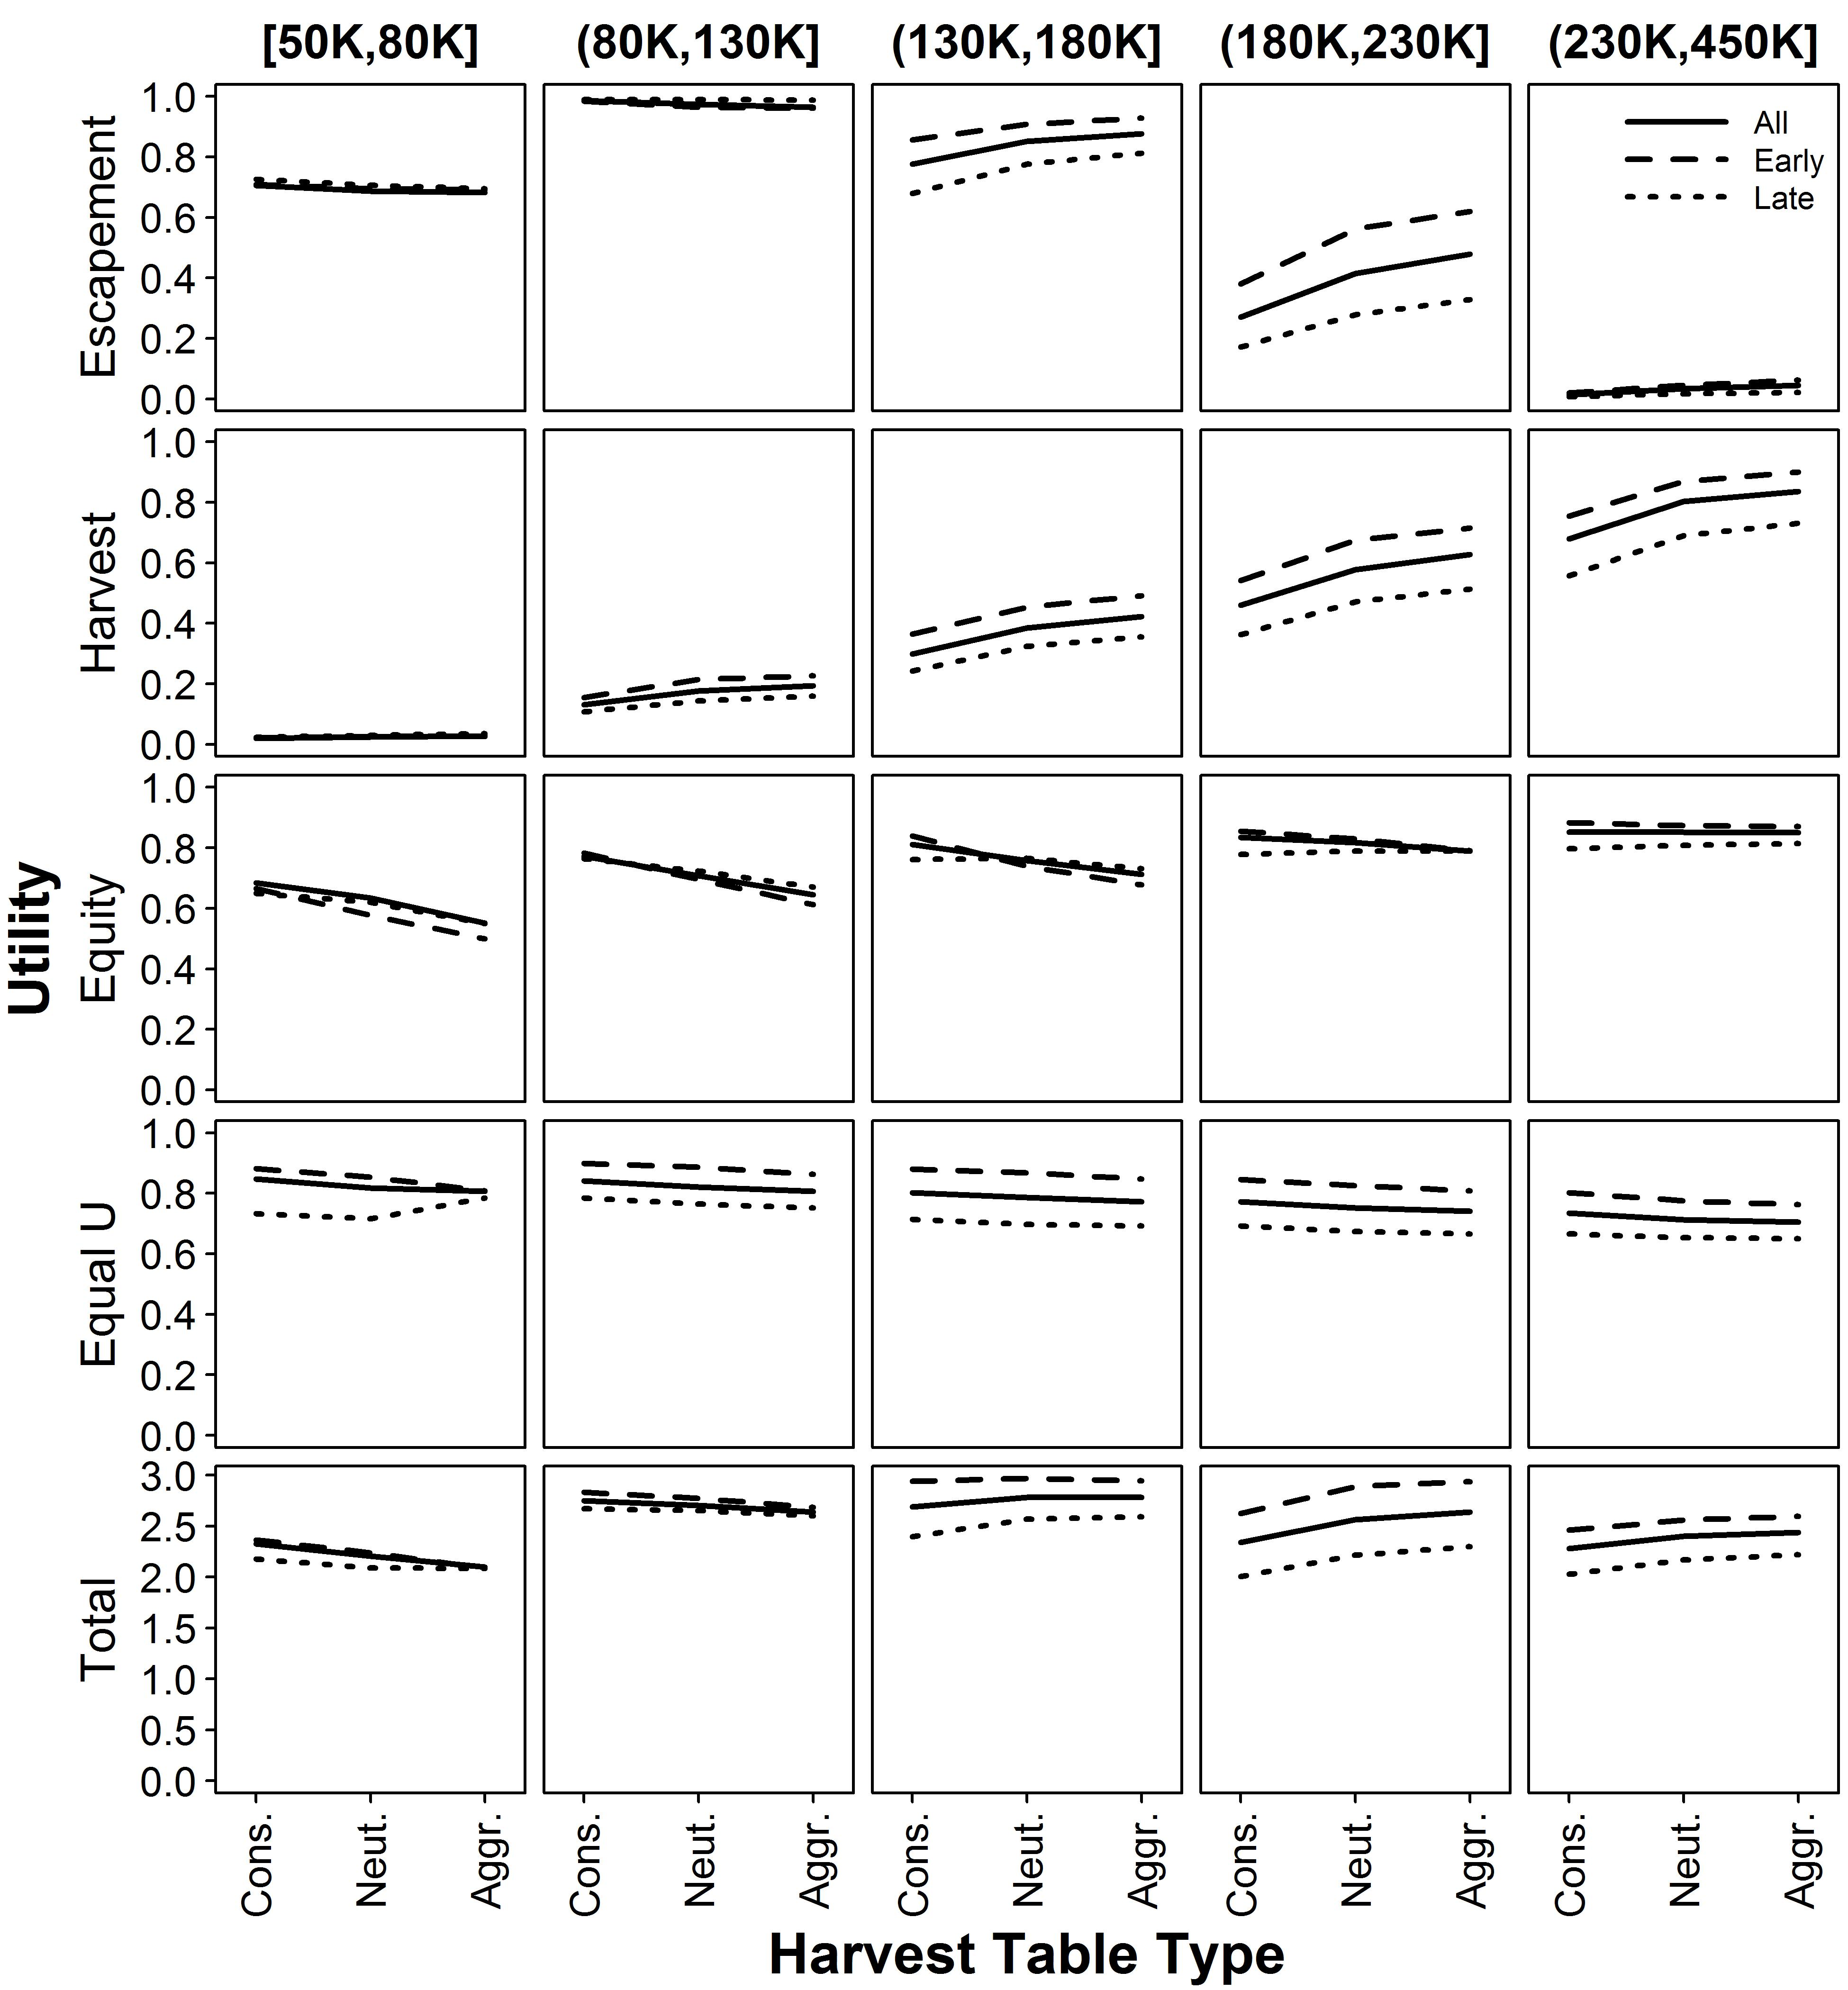
\includegraphics{img/Ch3/Values_4.jpg}
  \caption{Detailed performance of assessed Strategy \#4. The layout of panels in this figure is the same as in Figure \ref{fig:ms1-utilities}, only substrategies represent different harvest tables used to set the number of days of open fishing per week based on how many fish are targeted to be harvested that week (harvest tables shown in Figure \ref{fig:ms4-schedules}).}
  \label{fig:ms4-utilities}
\end{figure}

\clearpage
\begin{figure}
  \centering
  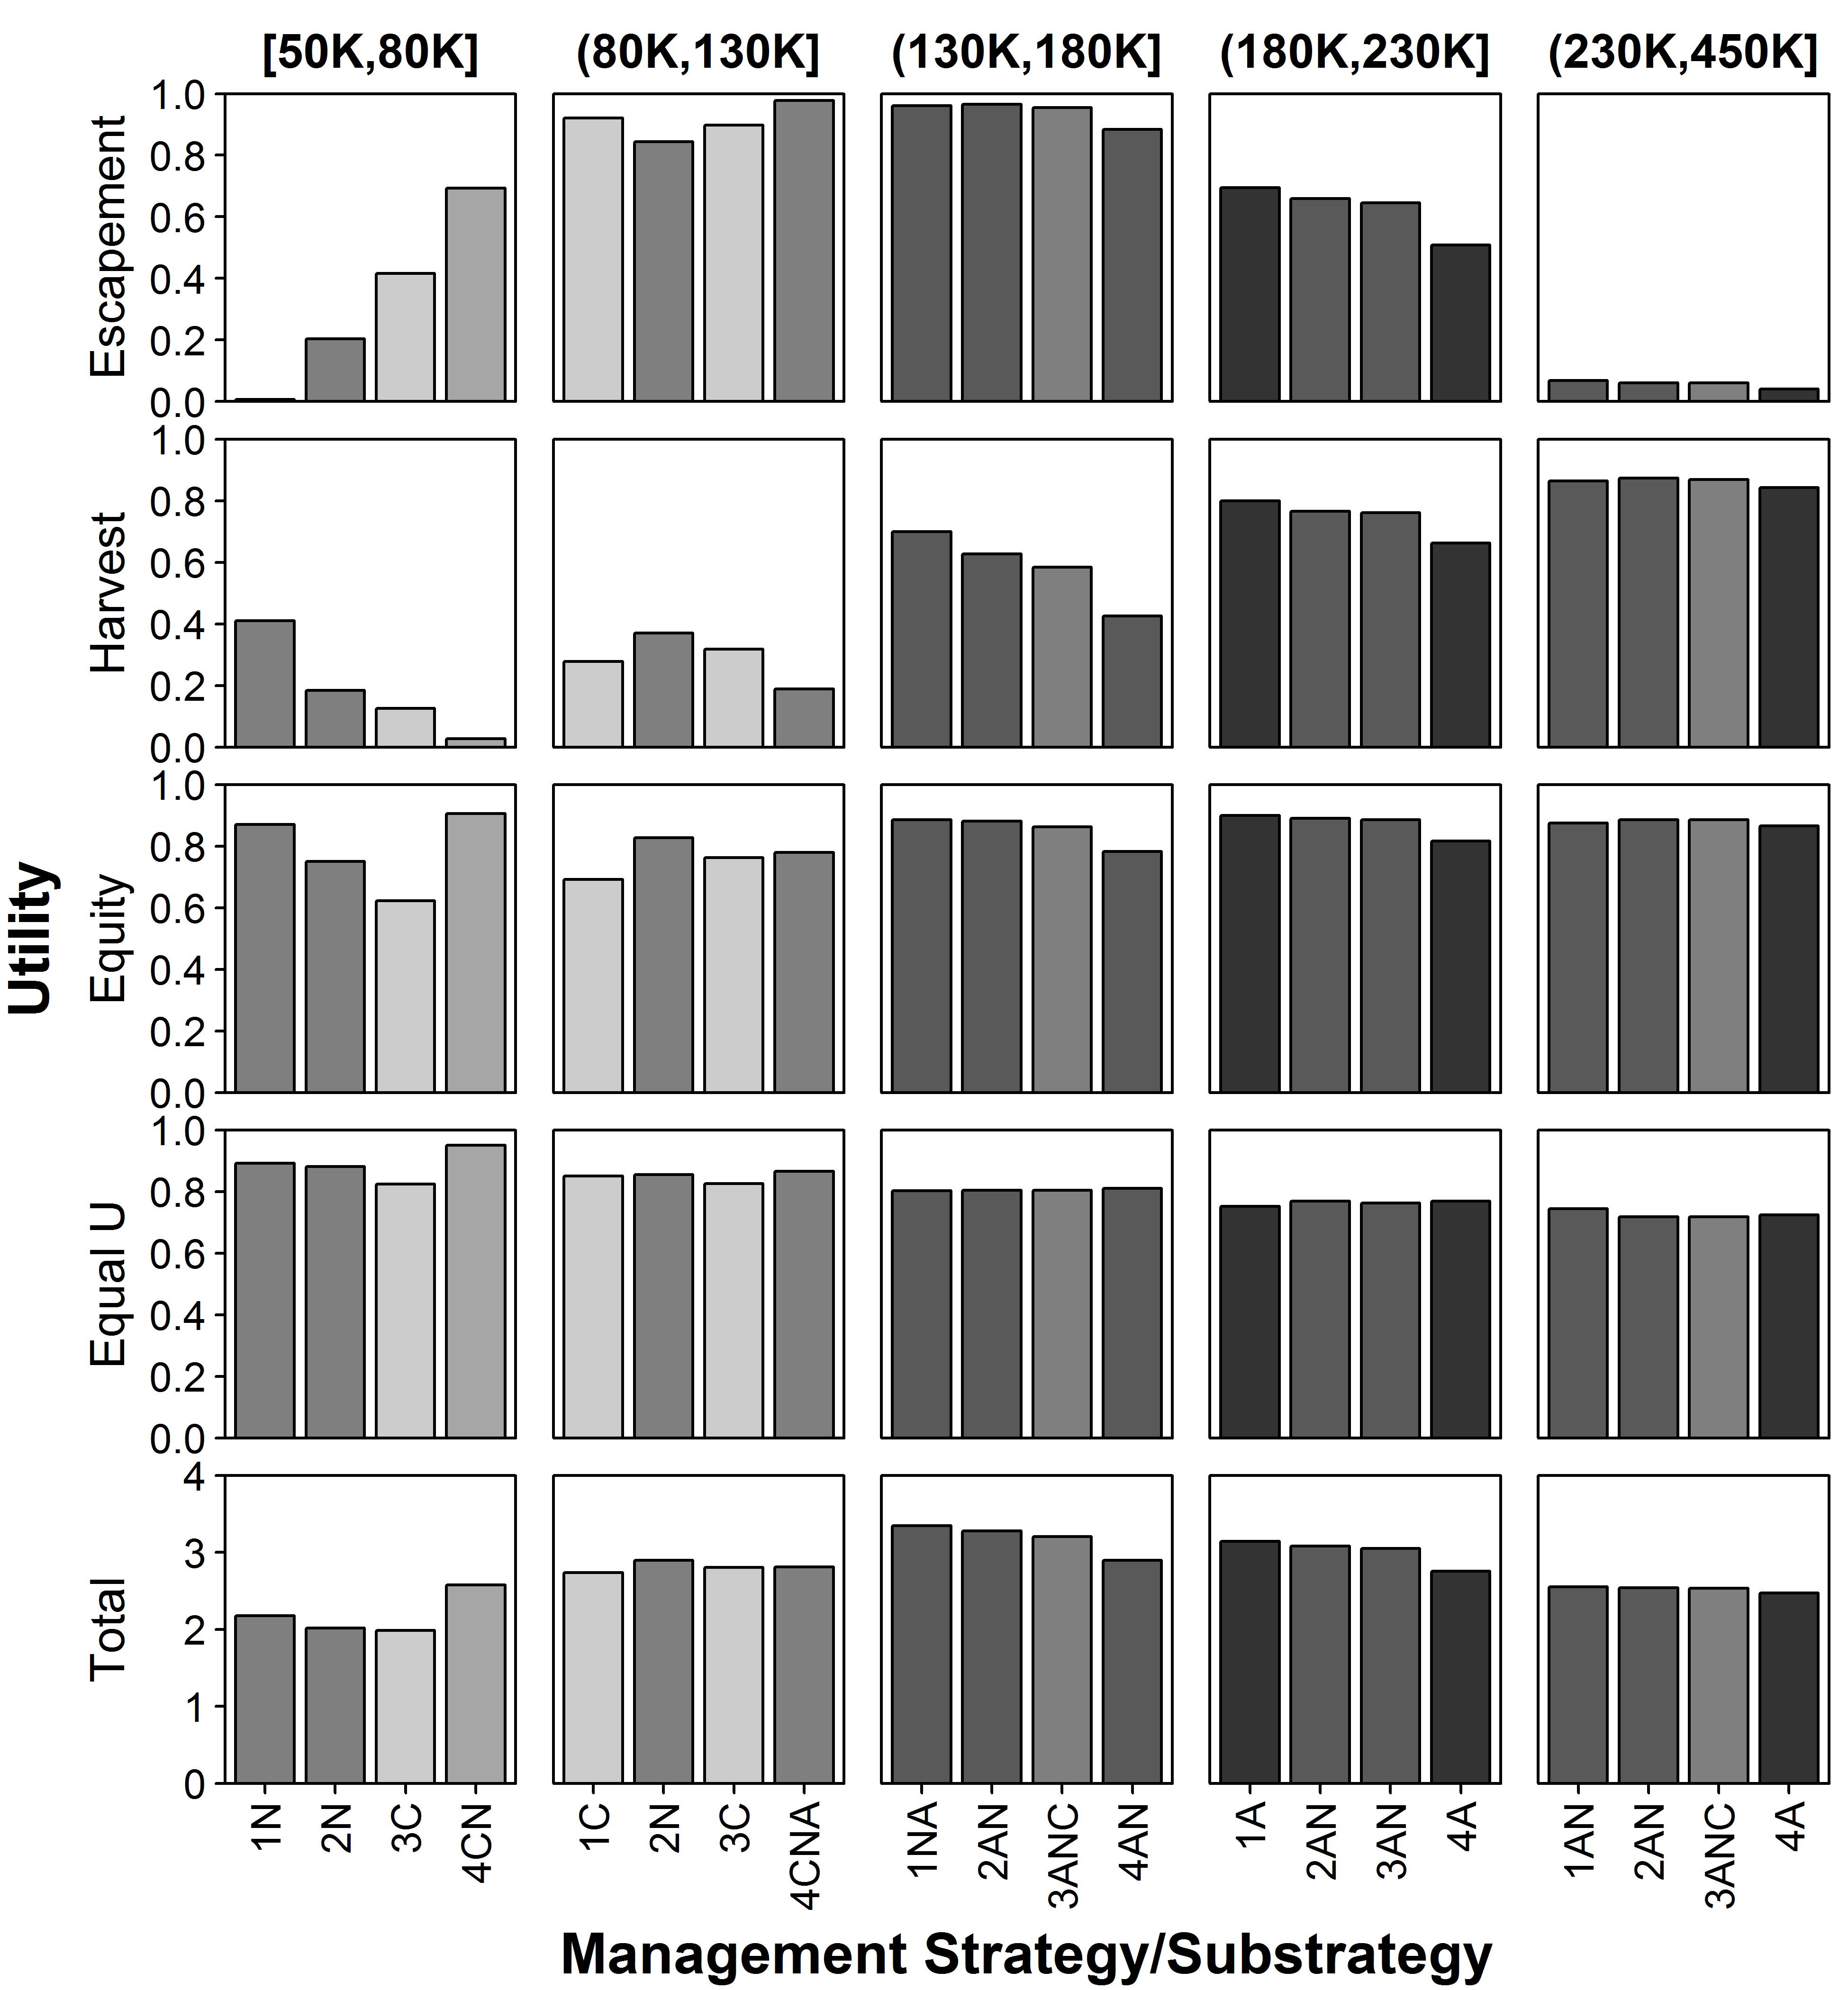
\includegraphics{img/Ch3/btwn-ms-utilities.jpg}
  \caption{Comparison of utility according to the different metrics between strategies (with the best substrategy selected for comparison) and run sizes. Numbers represent the strategy, letters and colors indicate the selected substrategy (darker colors represent more aggressive substrategies; C = conservative, N = neutral, A = aggressive; multiple letters indicate a tie). Total utility was calculated according to the default weighting scheme, where all objectives received equal weight.}
  \label{fig:btwn-ms-utilities}
\end{figure}

\begin{figure}
  \centering
  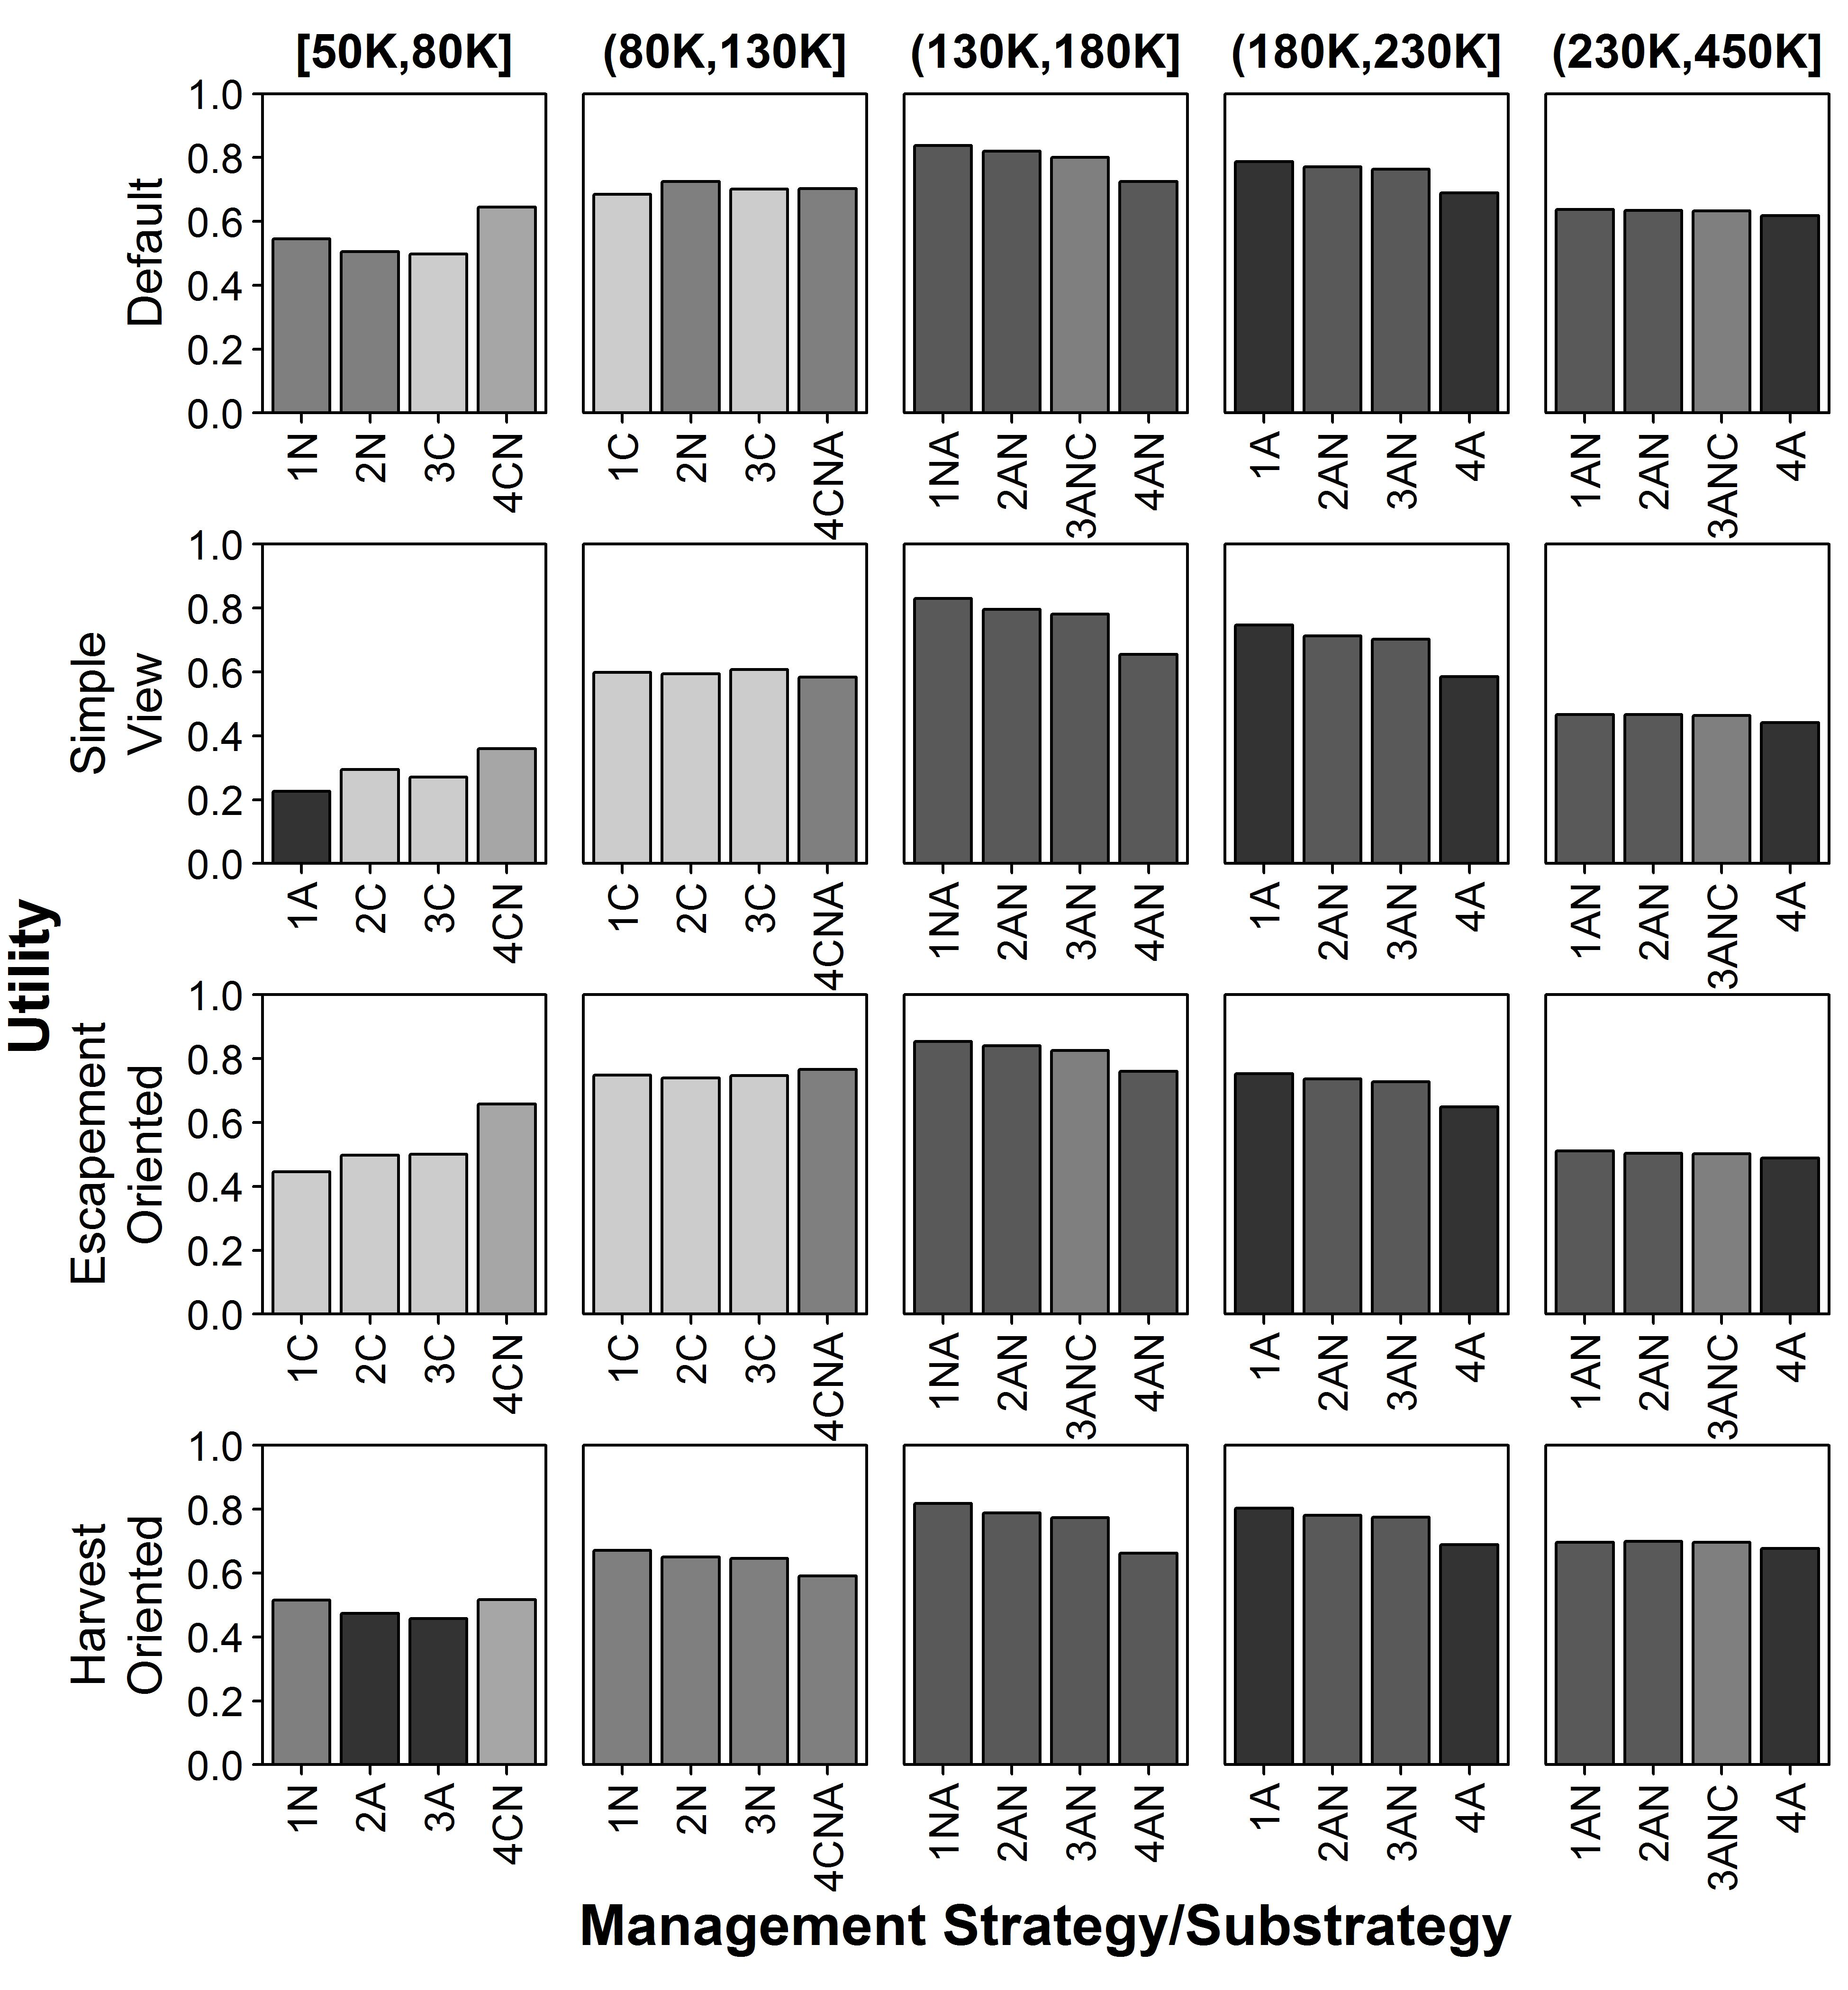
\includegraphics{img/Ch3/btwn-ms-weights.jpg}
  \caption{The total utility metric of the best-performing substrategy (letters/colors) for each strategy (numbers), when considering different weighting schemes (schemes described in Section \ref{alt-weights}). Bars are shaded based on the best substrategy, with darker greys representing more aggressive substrategies (C = conservative, N = neutral, A = aggressive; multiple letters indicate a tie). Total utility was scaled to the maximum attainable total utility for each weighting scheme, which is equal to the sum of the weights.}
  \label{fig:btwn-ms-weights}
\end{figure}

\end{singlespace}

\setlength{\parskip}{6pt plus 2pt minus 1pt}

\appendix


\captionsetup[figure]{list=yes} \captionsetup[table]{list=yes}

\chapter{Parameterization of the Operating Model in Chapter
\ref{ch3}}\label{appendix-a}

\noindent
There were two main components of the operating model that needed to be
parameterized based on observed information for it to adequately
represent the dynamics of the real Kuskokwim River subsistence salmon
fishery:

\begin{enumerate}
\def\labelenumi{(\arabic{enumi})}
\item
  \emph{Biological}: abundance, timing, spatial characteristics of the
  salmon populations (three Chinook salmon substocks and one aggregate
  stock of chum and sockeye salmon) and
\item
  \emph{Sociological}: spatial distribution of effort and desired/needed
  harvest and temporal aspects of the effort dynamics.
\end{enumerate}

\noindent
This appendix describes how empirical information collected in the
Kuskokwim River drainage was used to parameterize the operating model
used in the Chapter \ref{ch3} analysis.

\section{Biological quantities}\label{biological-quantities}

\subsection{Chinook salmon total abundance}\label{mse-data-N}

\noindent
Drainage-wide total Chinook salmon run abundance was informed by
\citet{liller-etal-2018}, which reported estimates in the years 1976 --
2017 from a maximum likelihood run reconstruction model. The model was
fitted to 20 escapement indices, commercial fishery
catch-per-unit-effort, and nine years of drainage-wide estimates of
total abundance obtained \emph{via} large-scale mark-recapture
experiments. Based on \citet{liller-etal-2018}, drainage-wide Chinook
salmon abundance has varied between 79,238 (in 2012) and 411,724 (in
1994), with a mean of 216,929 and standard deviation of 87,556. A kernel
density estimator was fitted to this distribution, and the cumulative
density function was obtained to allow sampling of continuous run sizes
in accordance with the historical frequency of run sizes (Figure
\ref{fig:N-plot}). The distribution was truncated at the smallest and
largest runs on record as of 2017 \(\pm\) 30,000 fish.

\subsection{Chinook salmon substock composition}\label{mse-data-pi}

\noindent
Substock composition, or the fraction of the aggregate Chinook salmon
run that was made up of fish from each substock, was informed by the
proportions of telemetry fish that spawned in each region in the years
2015 and 2016 \citep{smith-liller-2017a, smith-liller-2017b}. Although
telemetry data from 2003 -- 2007 were also available, only these years
were used because:

\begin{enumerate}
\def\labelenumi{(\arabic{enumi})}
\item
  they allowed the incorporation of information from lower river fish
  (as a result of the tagging location; see Section
  \ref{mse-data-ss-timing}) and
\item
  the management of the fishery resulted in less selection of upper
  river substocks in the harvest because fishing was pushed later in the
  season than in the 2003 -- 2007 block of years.
\end{enumerate}

\noindent
In each run of the operating model, a random Dirichlet vector was drawn
with parameter vector equal to {[}lower = 19, middle = 61, upper =
20{]}, which results in an expectation roughly equal to the average
contribution in 2015 and 2016. The use of a Dirichlet distribution with
these parameters generated a modest amount of variability around the
expected substock composition.

\subsection{Chinook salmon run timing}\label{chinook-salmon-run-timing}

\subsubsection{Aggregate timing}\label{aggregate-timing}

\noindent
Run timing information for the aggregate Chinook salmon stock was
available from the Bethel Test Fishery \citep{bue-lipka-2016}, which has
produced a daily value of catch-per-unit-effort for each day between
June 1 and August 24 for the years 1984 -- 2018. The estimates of
location (\(D_{50}\)) and inverse scale (\(h\)) of a logistic function
shown in Table \ref{tab:rt-ests-table} were used to quantify the timing
with which the simulated aggregate Chinook salmon stock runs through the
lower river.

\subsubsection{Substock-specific timing}\label{mse-data-ss-timing}

\noindent
The timing of the specific Chinook salmon substocks (i.e., those
spawning in lower, middle, and upper river tributaries) were informed by
radio telemetry studies
\citep{stuby-2007, smith-liller-2017a, smith-liller-2017b}. The tag date
and final tributary of each fish was available for the years 2003 --
2007 and 2015 -- 2016. In the first block of years, the tagging site was
located near Kalskag, which excluded any fish spawning in lower river
tributaries. In the second block of years, the tag site was moved near
the Johnson River, which allowed the inclusion of fish spawning in the
lower river tributaries. Logistic models \eqref{eq:logistic} were fitted
to the data from each substock and year separately to obtain estimates
of the \(D_{50}\) for each substock in each year data were available,
and differences in \(D_{50}\) for the middle river substocks and each of
the other substocks were calculated (Table \ref{tab:d50-devs-table}).
For parameterizing the run timing of middle river substocks, random
values drawn from the aggregate population estimates were used, and
random uniform deviations for the lower river and upper river \(D_{50}\)
were used in accordance with the deviations shown in Table
\ref{tab:d50-devs-table} (i.e., lower river substocks had a \(D_{50}\)
value that was anywhere between 0 and 3 days later than that of the
middle river, and upper river substocks had a value that was between 5
and 10 days earlier than middle river substocks.

\subsection{Spatial distribution of escapement}\label{calc-esc-p}

\noindent
Due to the spatial nature of the operating model, it was important to
capture the behavior of fish becoming invulnerable to harvest by
swimming up a spawning tributary. This aspect was informed using data
from the telemetry studies: it was possible to quantify the fraction of
all tagged fish that made it to a particular reach that ultimately
spawned in a tributary with a confluence in that reach in each year.
These fractions were averaged across years and the average was used to
dictate how many fish from each substock \(s\) in reach \(r\) on day
\(d\) would ``peel off'' from the mainstem into a tributary in that
reach on that day. For the aggregate chum/sockeye stock, which does not
have this kind of information, the substock structure was removed. These
estimates are shown in Table \ref{tab:esc-p-table}.

\subsection{Species ratios}\label{mse-data-ratios}

\noindent
Because chum and sockeye salmon lack the abundance data available for
Chinook salmon, their daily entry dynamics were modeled using observed
species ratios from the Bethel Test Fishery. These data were prepared by
taking the catch-per-unit-effort of chum salmon plus sockeye salmon, and
dividing it by the catch-per-unit-effort of Chinook salmon on each day
of each year for which data were available (assuming the subsistence
fishery uses the same gill net mesh sizes as the Bethel Test Fishery,
which is a largely valid assumption in recent years). This represents
how many vulnerable chum/sockeye salmon were available for harvest
relative to Chinook salmon. Daily values that couldn't be calculated
(i.e., when zero Chinook salmon were caught) were populated with the
average value for all years for which a species ratio could be
calculated on that same day. These annual time series were highly
variable from day to day, likely as a result of sampling variability, so
a cubic spline smoother was fitted to remove this variability. The time
series of smoothed ratios from all years is shown in Figure
\ref{fig:ratios-plot}.

In each simulated year, one randomly sampled annual time series was
selected to generate the daily species composition for that year. To
avoid anomalous outcomes, i.e., unlikely combinations of Chinook run
timing and abundance matched with very high or low species ratios in the
simulation. I investigated two historical variables for covariance with
the species ratio: \(D_{50}\) and total Chinook salmon run size using a
\(\chi^2\) test for independence. I categorized run timing, run size,
and the date at which a species ratio of 15:1 was observed into three
bins, with endpoints delineated by the 33\% and 66\% percentiles. I was
interested in whether Chinook salmon runs with different run timing or
size tended to coincide with attaining high species ratios earlier or
later in the season. If these sorts of patterns were present, they would
need to be accounted for in the simulation.

I found that the first date of 15:1 ratios and Chinook salmon run timing
had more non-independence (\(\chi^2 = 11, df = 4, p = 0.027\)) than
Chinook salmon run size (\(\chi^2 = 1.84, df = 4, p = 0.765\)). This
indicated that species ratios could be drawn independently with regards
to the simulated run size, but not the simulated run timing. As shown in
Table \ref{tab:ratio-timing-cov-table}, the probability of having early
high ratios has been historically highest in early Chinook runs. Late
Chinook salmon runs tended to occur in years that had later dates of
15:1. I incorporated these patterns in the simulation by first sampling
the run timing for that simulated year, then assigning it to a category,
then sampling a ratio category with probability equal to the appropriate
column in Table \ref{tab:ratio-timing-cov-table}. Finally, a year was
randomly selected from the approximately 10 years in that same category,
and the daily species ratios that year were used to drive the species
composition in that simulated year.

\section{Sociological quantities}\label{sociological-quantities}

\subsection{Needed salmon harvest by river reach}\label{mse-data-needs}

\noindent
The term ``minimally needed salmon harvest'' salmon harvest refers to
the amount of salmon that would satisfy the very basics of the
subsistence needs of fishers in the drainage -- without meeting this
level it is reasonable to assume the fishing population is experiencing
hardship. ``Maximally needed salmon harvest'' represents the salmon
harvest that would completely meet their needs (i.e., if they could
harvest as many fish as they would like). The Alaska Board of Fisheries
has produced ranges for each species, termed the ``Amounts Reasonably
Necessary for Subsistence'' (ANS) and represents the drainage-wide range
of harvest by species needed to sustain subsistence fishers each year.
These ANS ranges are 67,200 -- 109,800 for Chinook salmon and 73,400 --
175,100 for chum/sockeye salmon. In this analysis, the lower bound of
the ANS range was used to specify minimally needed salmon harvest by
species, and the upper bound of the range was used to specify maximally
needed salmon harvests. Minimal harvest needs were used to measure the
attainment of management objectives and maximally needed amounts were
used to drive the dynamics of the effort model.

However, these values are only available for the entire drainage -- they
are not partitioned to individual villages. For this analysis, a minimal
and maximal value was needed for the villages located within each reach.
The drainage-wide totals were thus partitioned by calculating the
average fraction that villages in each reach have harvested of the
drainage-wide. \citet{hamazaki-2011} present year-, species- and
village-specific salmon harvests for the period (1990 -- 2009), and data
through 2015 can be found in \citet{carroll-hamazaki-2012},
\citet{shelden-etal-2014}, \citet{shelden-etal-2015},
\citet{shelden-etal-2016a}, and \citet{shelden-etal-2016b}. Only years
1990 -- 2000 were included for the spatial distribution of salmon need
because stakeholders indicated the restrictions in recent years make the
harvest proportions non-representative and that the earlier years are
more reflective of how harvest should be distributed. The partitioned
values by species are shown in Table \ref{tab:socio-spatial-table}.

\subsection{Maximum daily effort by river reach}\label{mse-data-effort}

\noindent
A key aspect of the sociological component to the operating model was
the spatial distribution of maximum fishing effort, i.e., the greatest
number of boat days that can be exerted by villages in each reach when
the fishery is open. This maximum effort was altered as the simulated
salmon season progressed based on the effort response submodel. The
important characteristic to capture is the proportion of all effort that
is attributable to each reach, i.e.~the scale is not important as the
efficiency of any one unit can be adjusted by altering the \(q\)
parameter. To determine how effort should be apportioned to each reach,
I devised a simple index of effort for each village and year based on
the number of reported fishing households. The Alaska Department of Fish
and Game has collected this information since 1990, and it is presented
in the same studies that quantified subsistence harvest patterns:
\citet{hamazaki-2011}, \citet{carroll-hamazaki-2012},
\citet{shelden-etal-2014}, \citet{shelden-etal-2015},
\citet{shelden-etal-2016a}, and \citet{shelden-etal-2016b}. The data
were reported as the number of households that ``usually fish'' and the
number of households that ``do not usually fish'' as surveyed each year
(as well as the number of ``unknown'' fishing status households). First,
I apportioned any unknown households probabilistically to the other two
categories by assuming the information was missing at random: if 60\% of
the fishing households belonged to the ``usually fishes'' category in a
village in a year, I apportioned 60\% of the unknown households to
``usually fishes'' and 40\% to ``does not usually fish''. I then
calculated the effort index for each village as 1 \(\times\) \# usually
+ 0.5 \(\times\) \# not usually, summed the values across villages
within each reach and year, calculated the annual proportion belonging
in each reach, and averaged these values across years.

\clearpage
\singlespacing

\begin{longtable}[t]{>{\bfseries}lcclcclcc}
\caption{\label{tab:d50-devs-table}Difference between $D_{50}$ for tagged fish destined for lower or upper river tributaries and those destined for middle river tributaries. These estimates were used to inform Chinook salmon substock-specific run timing.}\\
\toprule
\textbf{Year} & \textbf{Lower} & \textbf{Upper}\\
\midrule
2003 &  & -2.0\\
2004 &  & -9.5\\
2005 &  & -4.9\\
2006 &  & -7.8\\
2007 &  & -2.5\\
\addlinespace
2015 & -0.7 & -10.7\\
2016 & 2 & -9.8\\
\bottomrule
\end{longtable}

\clearpage

\begin{longtable}[t]{clccccclccccclccccclccccclccccclcccc}
\caption{\label{tab:esc-p-table}Spatial distribution of escapement in the operating model. The number in each cell represents $\psi_{r,s}$: the fraction of fish from a stock that make it to a reach and survive the fishery that ultimately escape and spawn in a tributary with a confluence with the main stem Kuskokwim located in that reach. These estimates were obtained from radio telemetry studies as described in Section \ref{calc-esc-p}, and the chum/sockeye salmon estimates were obtained by removing the substock structure from the Chinook salmon data.}\\
\toprule
\multicolumn{1}{c}{\bfseries } & \multicolumn{1}{c}{\bfseries } & \multicolumn{3}{c}{\bfseries Chinook Salmon} & \multicolumn{1}{c}{\bfseries } \\
\cmidrule(l{2pt}r{2pt}){3-5}
\textbf{Reach \#} & \textbf{Tributaries in Reach} & \textbf{Lower} & \textbf{Middle} & \textbf{Upper} & \textbf{Chum/Sockeye}\\
\midrule
\addlinespace[0.3em]
\multicolumn{36}{l}{\textbf{Lower River}}\\
\hline
\hspace{1em}4 & Kwethluk & 65.3\% & 0\% & 0\% & 12.4\%\\
\hspace{1em}5 & Kasigluk, Kisaralik & 80.1\% & 0\% & 0\% & 6\%\\
\hspace{1em}6 & Tuluksak & 100\% & 0\% & 0\% & 1.7\%\\
\addlinespace[0.3em]
\hline
\multicolumn{36}{l}{\textbf{Middle River}}\\
\hline
\hspace{1em}9 & Aniak & 0\% & 28.1\% & 0\% & 24.6\%\\
\hspace{1em}10 & Owhat & 0\% & 0.5\% & 0\% & 0.4\%\\
\hspace{1em}11 & Holokuk, Sue Creek, Veahna & 0\% & 3.7\% & 0\% & 3.4\%\\
\hspace{1em}12 & Oskawalik & 0\% & 2.7\% & 0\% & 2.4\%\\
\hspace{1em}13 & Crooked Creek, George & 0\% & 6\% & 0\% & 4.8\%\\
\hspace{1em}15 & Vreeland, Holitna & 0\% & 77.3\% & 0\% & 64.6\%\\
\hspace{1em}16 & Stony & 0\% & 32.8\% & 0\% & 25.8\%\\
\hspace{1em}17 & Swift, Tatlawiksuk & 0\% & 100\% & 0\% & 55.9\%\\
\addlinespace[0.3em]
\hline
\multicolumn{36}{l}{\textbf{Upper River}}\\
\hline
\hspace{1em}20 & Selatna, Black & 0\% & 0\% & 6\% & 6\%\\
\hspace{1em}22 & Takotna & 0\% & 0\% & 17.5\% & 17.5\%\\
\hspace{1em}24 & Middle Fork & 0\% & 0\% & 94\% & 94\%\\
\hspace{1em}26 & South Fork, East Fork & 0\% & 0\% & 100\% & 100\%\\
\bottomrule
\end{longtable}

\clearpage

\begin{table}

\caption{\label{tab:ratio-timing-cov-table}Non-independence of historically-observed Chinook salmon run timing and the date at which the species ratio of 15:1 chum+sockeye:Chinook was obtained. Columns sum to one and represent the empirical probability of observing a ratio type in each of the three categories along the rows. Independence would have all cells equal to 33.3\% -- note that early high ratios tend to occur in years with early Chinook salmon runs, and \textit{vice versa}.}
\centering
\begin{tabular}[t]{>{\bfseries}lccclccclccclccc}
\toprule
\multicolumn{1}{c}{\bfseries } & \multicolumn{3}{c}{\bfseries Chinook Salmon Run Timing} \\
\cmidrule(l{2pt}r{2pt}){2-4}
\textbf{Ratio Category} & \textbf{Earliest 33\%} & \textbf{Middle 33\%} & \textbf{Latest 33\%}\\
\midrule
Earliest 33\% & 66.7\% & 11.1\% & 20\%\\
Middle 33\% & 33.3\% & 44.4\% & 20\%\\
Latest 33\% & 0\% & 44.4\% & 60\%\\
\bottomrule
\end{tabular}
\end{table}

\clearpage

\begin{landscape}\begin{table}

\caption{\label{tab:socio-spatial-table}Key sociological quantities used in the operating model, broken down by spatial area (reach). Each reach is 35 km in main stem river length. Effort ($E_{\text{MAX},r}$) is expressed as the maximum number of boats fishing per day in reach $r$. The \% columns represent the average fraction of the total harvest by species that was harvested by villages within each reach over the period 1990 -- 2000. Harvest values have been rounded to the nearest 100 for ease of presentation, but the total column represents the sum of non-rounded quantities. Although these data were available through 2015, region stakeholders indicated that the recent years have been contaminated by harvest restrictions, and that these earlier years would be more representative.}
\centering
\begin{tabular}[t]{lllllllll}
\toprule
\multicolumn{1}{c}{\bfseries } & \multicolumn{1}{c}{\bfseries } & \multicolumn{1}{c}{\bfseries } & \multicolumn{3}{c}{\bfseries Chinook Salmon} & \multicolumn{3}{c}{\bfseries Chum/Sockeye Salmon} \\
\cmidrule(l{2pt}r{2pt}){4-6} \cmidrule(l{2pt}r{2pt}){7-9}
\textbf{Reach \#} & \textbf{Villages in Reach} & \textbf{Effort} & \textbf{\%} & \textbf{Min.} & \textbf{Max.} & \textbf{\%} & \textbf{Min.} & \textbf{Max.}\\
\midrule
\addlinespace[0.3em]
\multicolumn{9}{l}{\textbf{Lower River}}\\
\hline
\hspace{1em}1 & Tuntutuliak, Eek & 42 & 7.6\% & 5,100 & 8,300 & 6.2\% & 4,600 & 10,900\\
\hspace{1em}2 & Atmautluak, Kasigluk, Nunapitchuk & 74 & 11\% & 7,400 & 12,000 & 13.6\% & 10,000 & 23,900\\
\hspace{1em}3 & Napakiak, Napaskiak, Oscarville, Bethel & 415 & 40.5\% & 27,200 & 44,500 & 34.1\% & 25,000 & 59,600\\
\hspace{1em}4 & Kwethluk, Akiachak & 74 & 17.2\% & 11,600 & 18,900 & 15.2\% & 11,200 & 26,600\\
\hspace{1em}5 & Akiak & 18 & 4.3\% & 2,900 & 4,800 & 4.9\% & 3,600 & 8,600\\
\hspace{1em}6 & Tuluksak & 21 & 3.9\% & 2,600 & 4,300 & 4.4\% & 3,300 & 7,800\\
\addlinespace[0.3em]
\hline
\multicolumn{9}{l}{\textbf{Middle River}}\\
\hline
\hspace{1em}8 & Lower Kalskag, Upper Kalskag & 33 & 5.1\% & 3,400 & 5,600 & 4.2\% & 3,100 & 7,400\\
\hspace{1em}9 & Aniak & 46 & 4.2\% & 2,800 & 4,600 & 4.6\% & 3,400 & 8,100\\
\hspace{1em}10 & Chuathbaluk & 9 & 1.3\% & 900 & 1,400 & 2.1\% & 1,600 & 3,700\\
\hspace{1em}13 & Crooked Creek & 9 & 1\% & 600 & 1,100 & 1.5\% & 1,100 & 2,600\\
\hspace{1em}14 & Red Devil & 6 & 0.3\% & 200 & 400 & 1.1\% & 800 & 2,000\\
\hspace{1em}15 & Sleetmute & 12 & 1.1\% & 800 & 1,200 & 2.1\% & 1,500 & 3,600\\
\hspace{1em}16 & Lime Village, Stony River & 10 & 0.7\% & 500 & 700 & 4\% & 3,000 & 7,000\\
\addlinespace[0.3em]
\hline
\multicolumn{9}{l}{\textbf{Upper River}}\\
\hline
\hspace{1em}22 & McGrath, Nikolai, Takotna, Telida & 42 & 1.7\% & 1,100 & 1,800 & 1.9\% & 1,400 & 3,300\\
\textbf{\hspace{1em}Total} & \textbf{} & \textbf{800} & \textbf{100\%} & \textbf{67,200} & \textbf{109,800} & \textbf{100\%} & \textbf{73,400} & \textbf{175,100}\\
\bottomrule
\end{tabular}
\end{table}
\end{landscape}

\clearpage

\begin{figure}
  \centering
  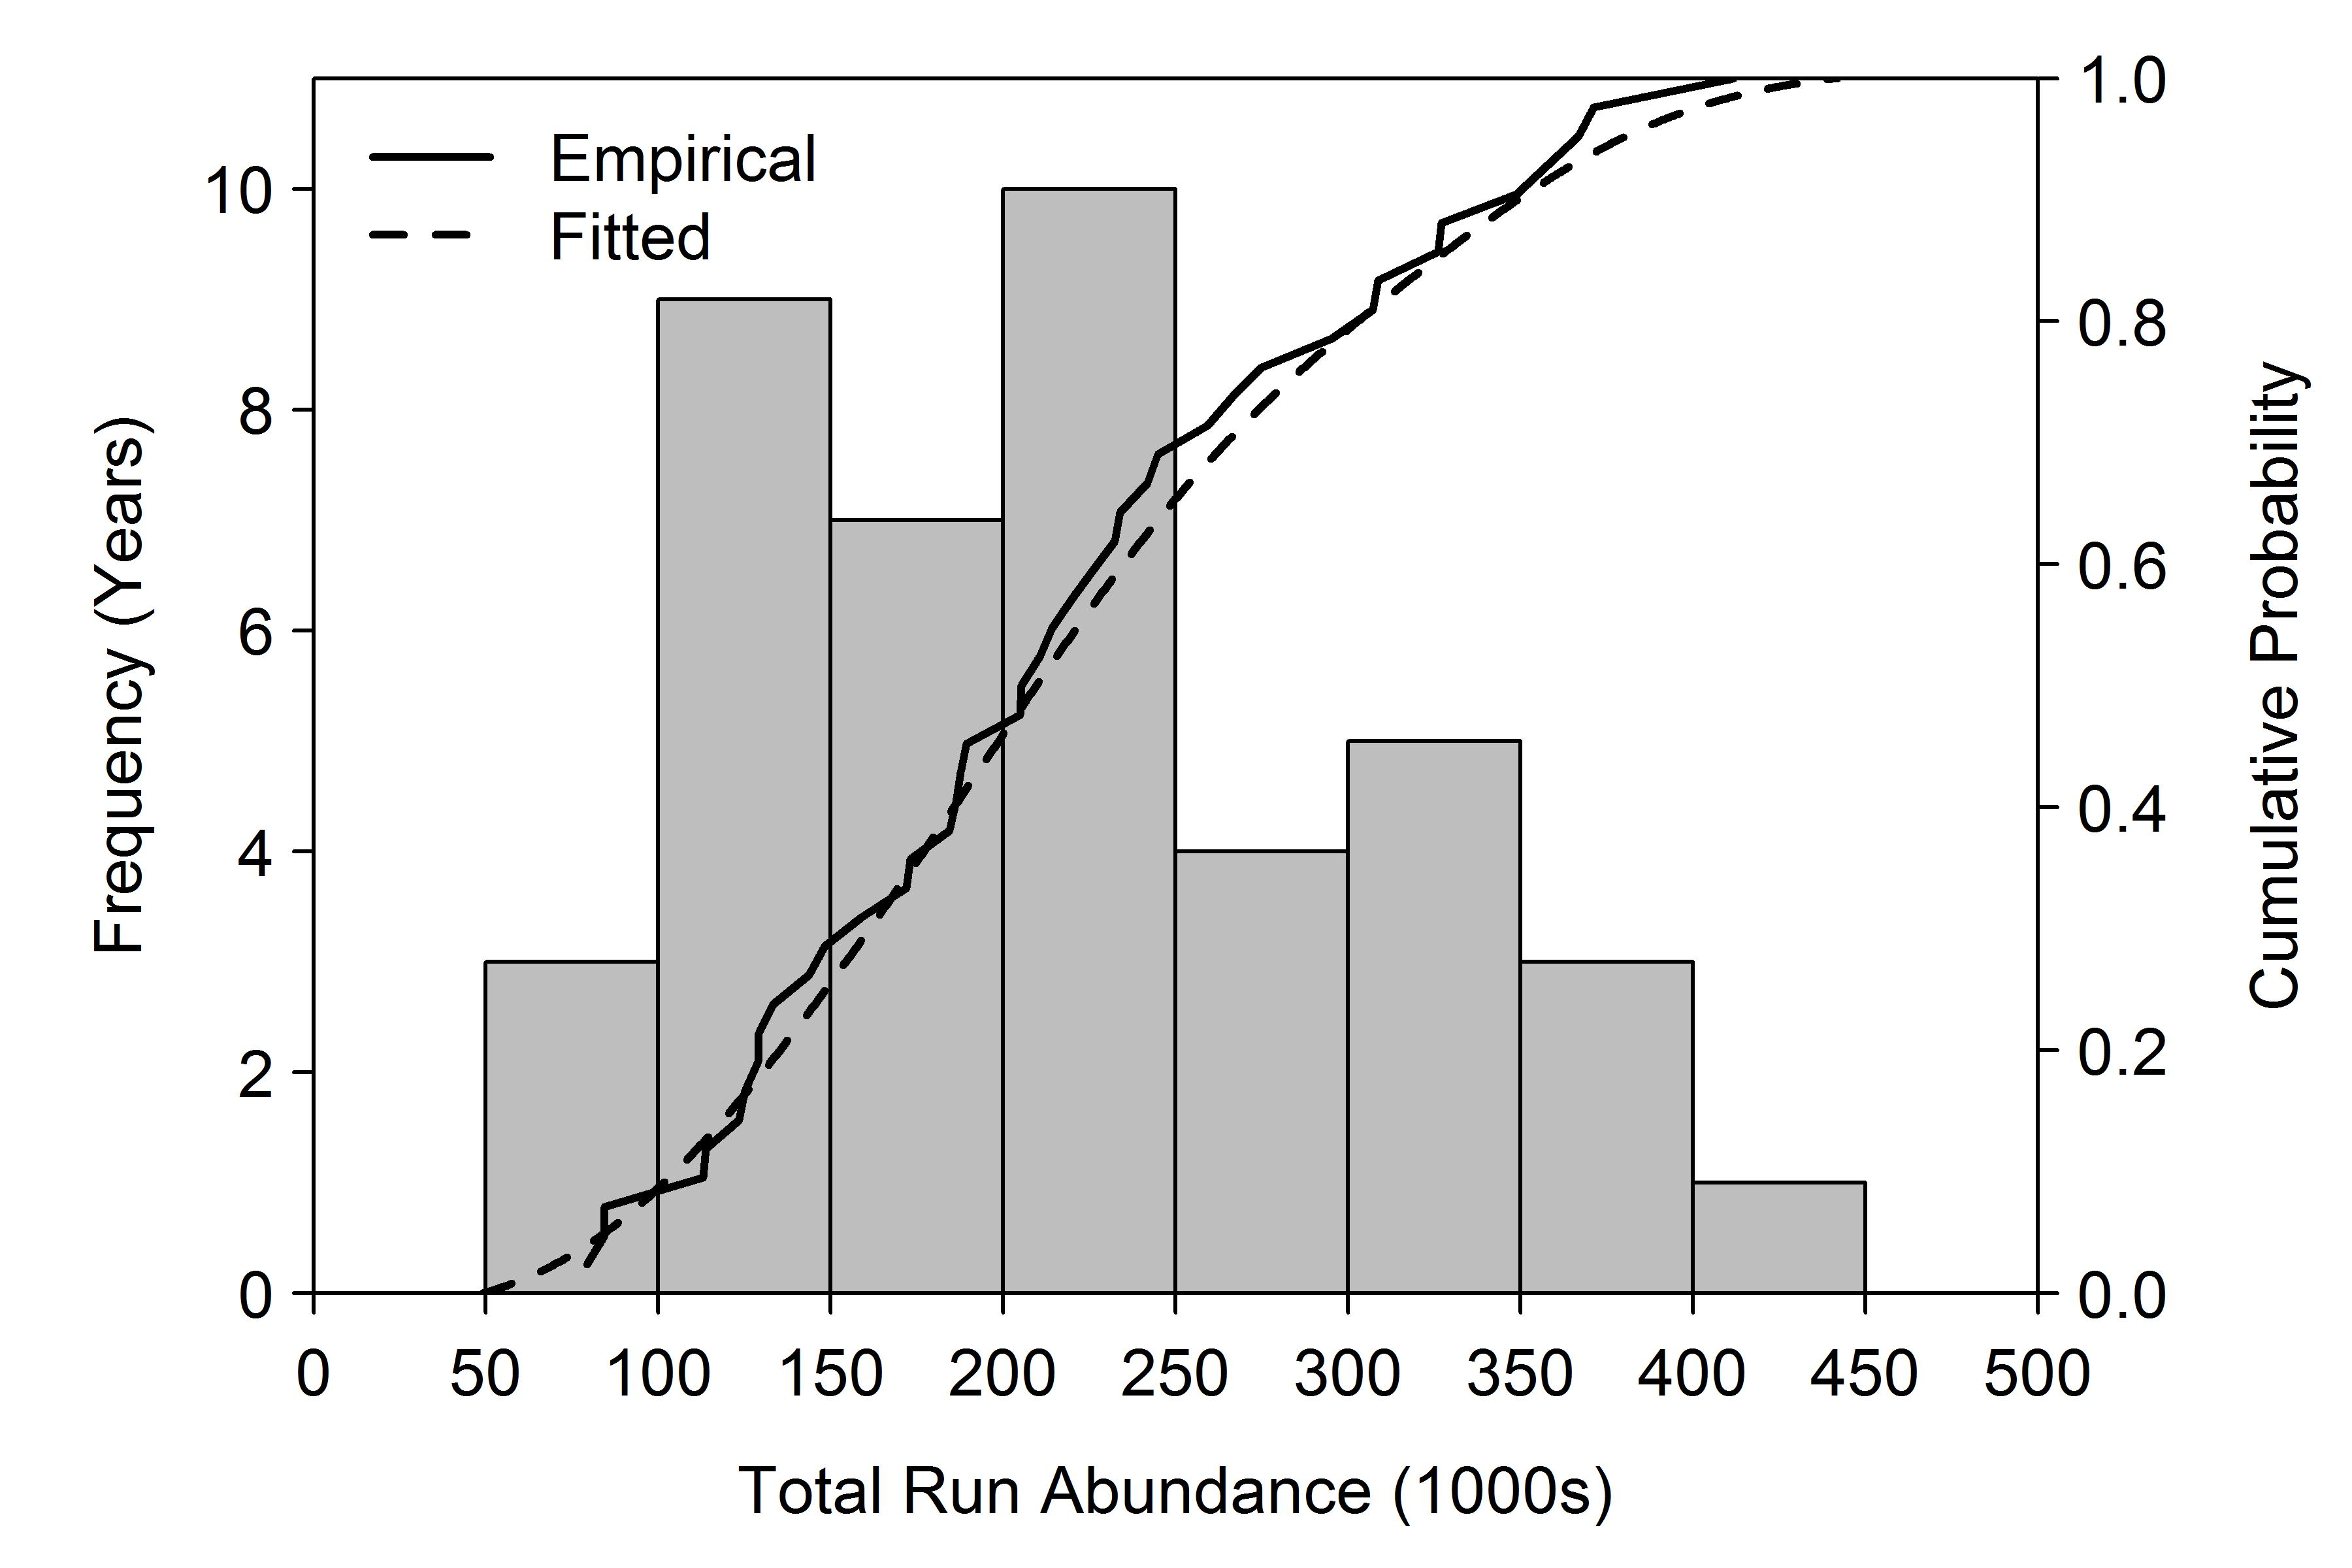
\includegraphics{img/Ch3/N-plot.jpg}
  \caption{Distribution of total drainage-wide run size for Kuskokwim River Chinook salmon, as presented in \cite{liller-etal-2018}. This distribution was used to generate the run size of the aggregate Chinook salmon populations entering the fishery system in a simulated year. The secondary $y$-axis represents the probability of a run falling below a given run size according to the historical frequency of run sizes; where the solid line shows the empirical cumulative distribution function and the dashed line shows one obtained by fitting a kernel density smoother to the empirical data. The fitted distribution was used for simulation to prevent the same 42 run size values from being replicated in the analysis.}
  \label{fig:N-plot}
\end{figure}

\clearpage

\begin{figure}
  \centering
  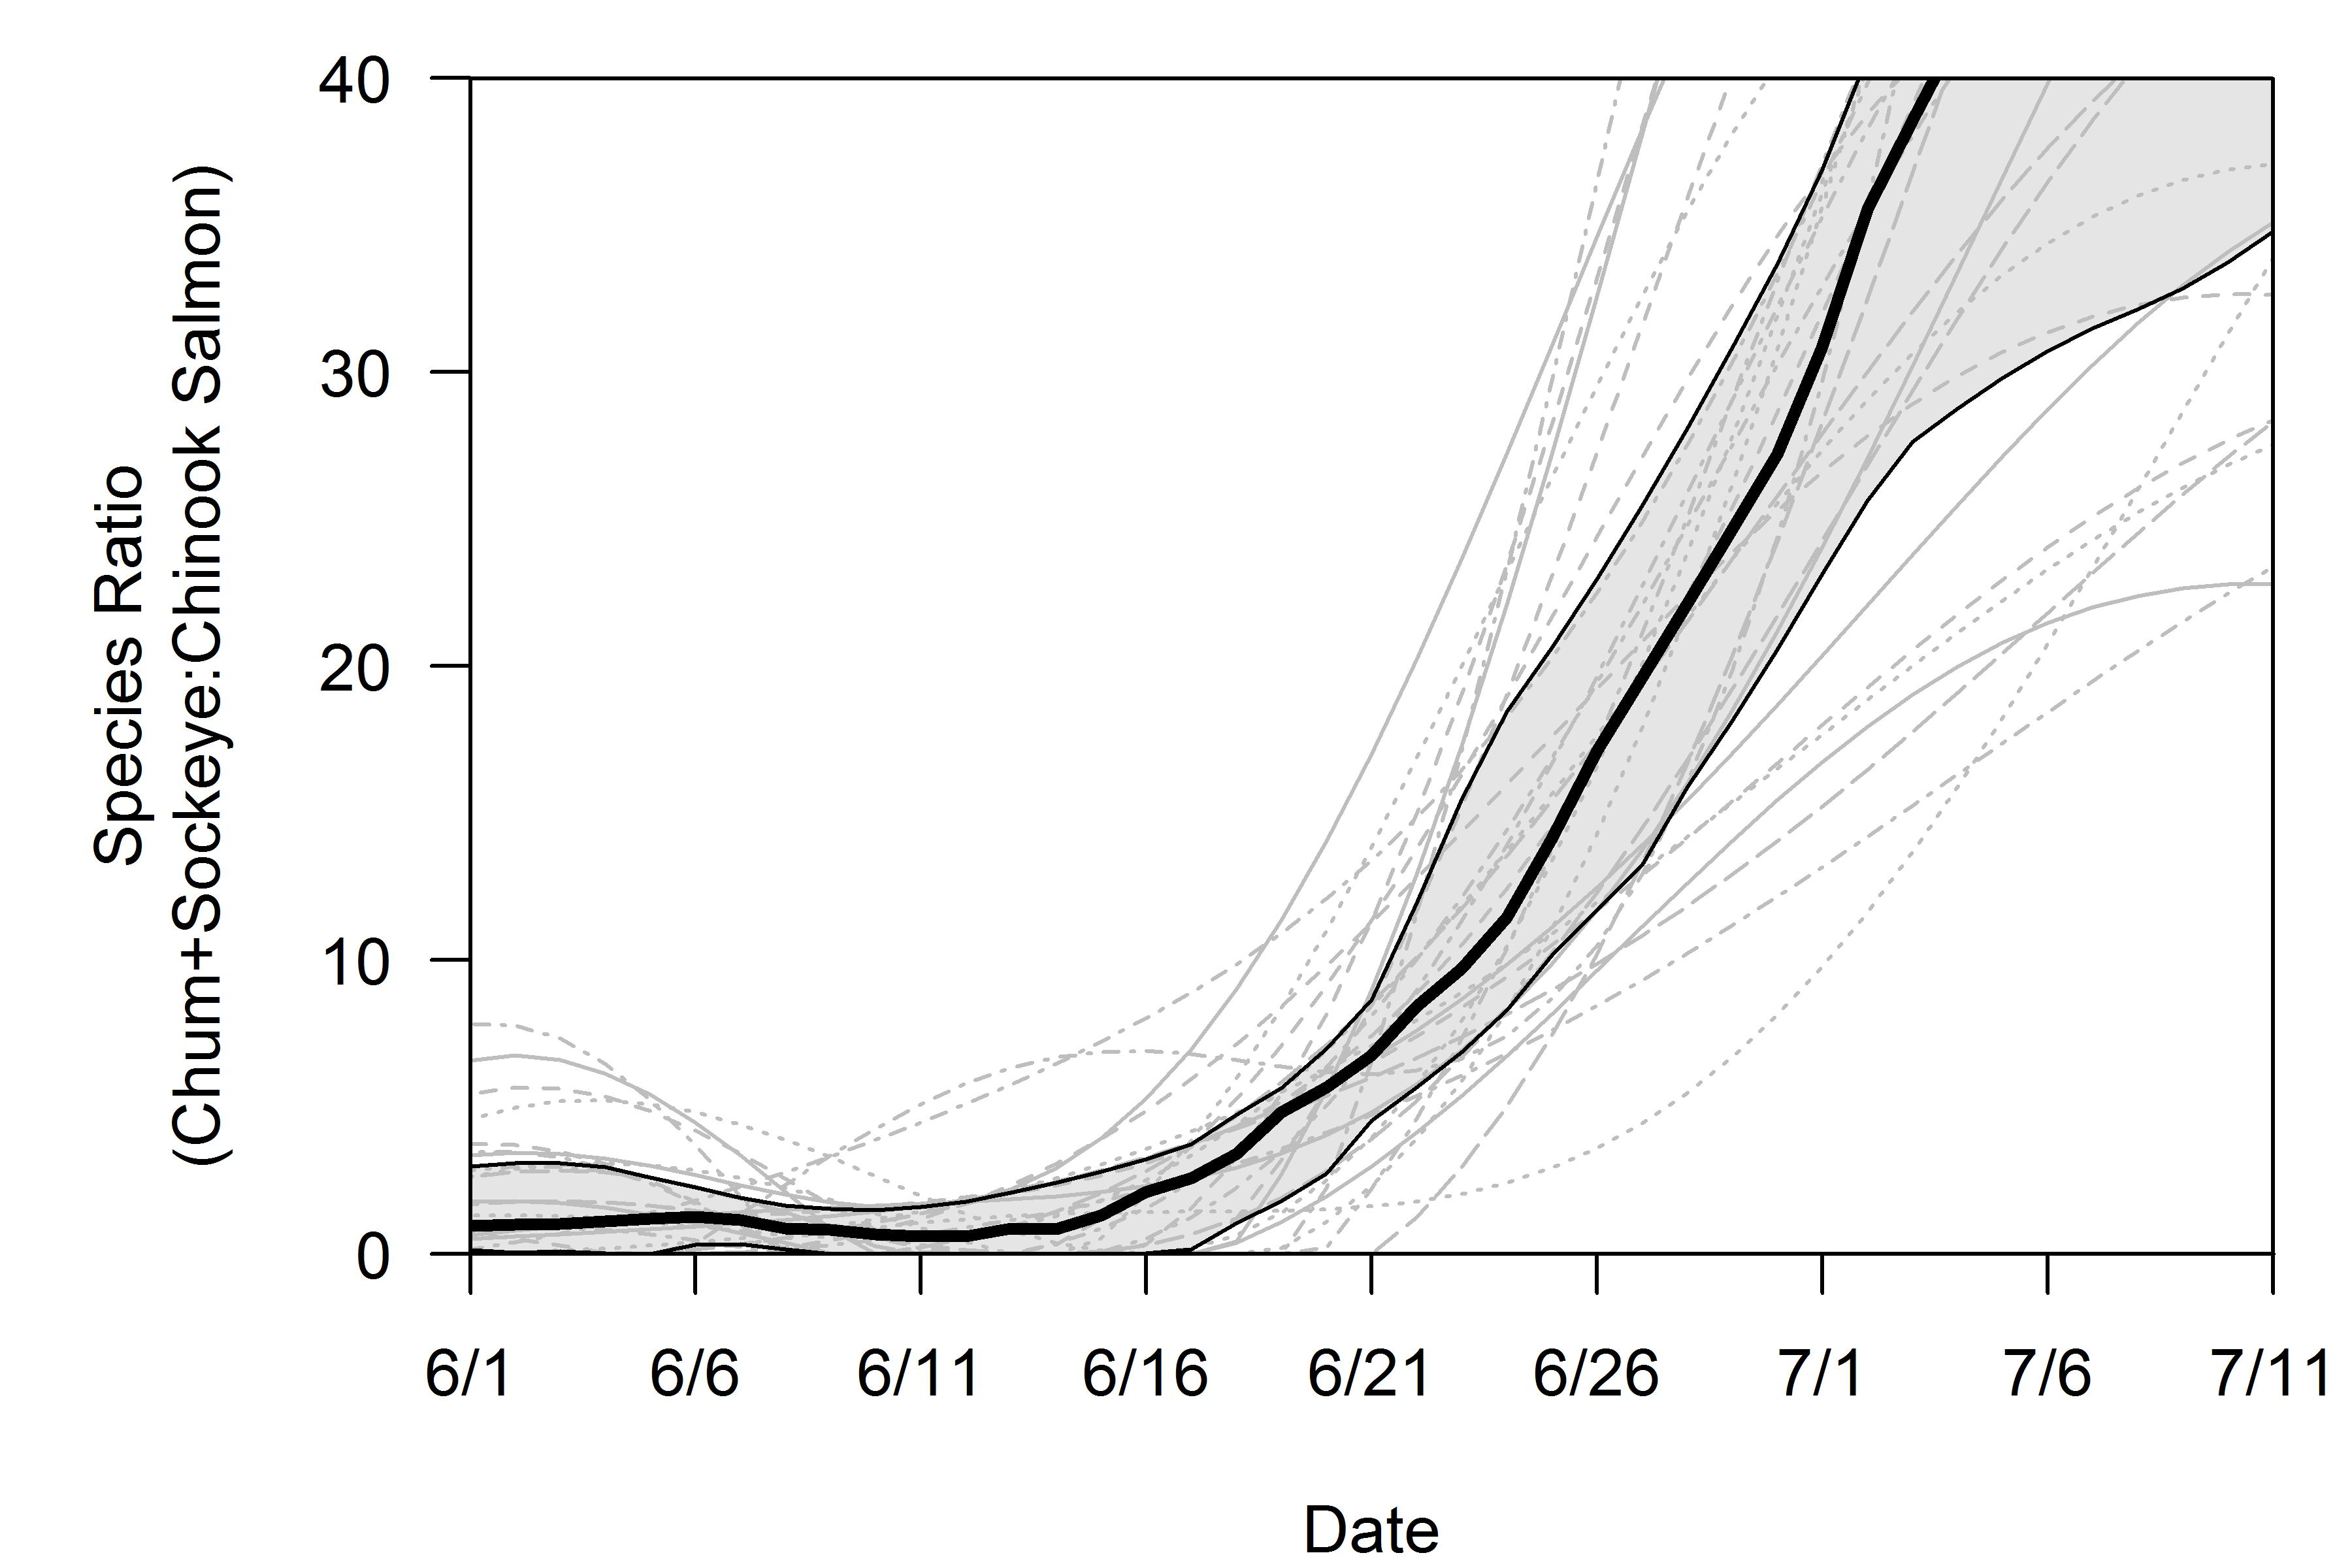
\includegraphics{img/Ch3/ratios-plot.jpg}
  \caption{Smoothed species ratios of chum+sockeye:Chinook salmon as detected by the Bethel Test Fishery. Individual grey lines represent separate years from 1984 -- 2017, the grey region represents the central 50\% of all smoothed ratios on each day and the thick black line represents the daily median. Only this time period is shown because at ratios larger than 20, the differences in the influence of chum/sockeye salmon on Chinook salmon harvest by the subsistence fishery are negligable.}
  \label{fig:ratios-plot}
\end{figure}

\clearpage

\doublespacing

\chapter{Validation of the Operating Model in Chapter
\ref{ch3}}\label{appendix-b}

For any simulation model used in the context of Management Strategy
Evaluation, the reliability of inferences drawn will be conditional on
the ability of the model components to capture the important behavioral
properties of the real system. Here, I provide a brief validation that
the fishery component of the operating model does in fact provide a
reasonable model of the real system when the fishery was unrestricted.

First, I thought it important that the model be able to replicate the
relationship between total Chinook salmon run size and total subsistence
salmon harvest. Capturing this pattern was important to ensure that the
fishery would not inadvertently harvest an unrealistically large or
small amount of fish in different run sizes if management mistakes were
made, which would confound my conclusions. As shown in Figure
\ref{fig:HvN}, this historical relationship has been quite noisy for the
observed historical time series, though an increasing pattern has
emerged: in general, more fish have been harvested in years with large
runs than years with small runs. I found that by tuning the catchability
(\(q\)) and effort response coefficients, I was able to reproduce the
pattern and variability quite well. Additionally, the scale and
variability of modeled chum/sockeye harvests were also similar to the
historically-observed distribution \ref{fig:chsk-harvest} -- this was
not key given chum/sockeye harvests did not inform any objectives, but
the agreement contributes more evidence that the effort response model
was adequately calibrated.

The next behavior of interest was the spatiotemporal distribution of
harvest. Because in-river salmon fisheries are sequential, fish
harvested in one area are invulnerable to harvest (and escapement) in
upriver areas. It also means that communities in downriver communities
may finish fishing earlier in the season because they are the first to
experience favorable fishing conditions (i.e., high in-river abundance
and resulting catch rates; in the Kuskokwim River drying weather also
plays an important role). If the timing of harvest was not captured
adequately, this would be an indication that the effort response
coefficients were improperly tuned and could result in unrealistic
conclusions. The patterns and variability in the day of the year at
which various percentiles of Chinook salmon harvest was attained by
reach compared between observed data and the modeled outcomes are shown
in Figure \ref{fig:temporal-harvest}. It seems that the patterns and
variability in harvest timing were reasonably well-captured,
particularly for downriver reaches. Reaches 14, 15, 16 and 22 seemed to
have had the largest deviations between observed and modeled patterns,
but given communities in these reaches harvest a negligible amount of
Chinook salmon in comparison to the downriver villages (Figure
\ref{fig:spatial-harvest}), I was not concerned by this finding.

The final important characteristic was the spatial distribution of
end-of-season harvest. Accurately representing this component of the
system would further indicate model adequacy. Figure
\ref{fig:spatial-harvest}) shows a comparison of the proportion of total
drainage-wide Chinook salmon subsistence harvest attributable to
communities in each reach between observed and modeled outcomes. While
the overall pattern was fully captured, there were moderate deviations
between the model and observations in reaches 2, 3, and 4.

\clearpage

\begin{figure}
  \centering
  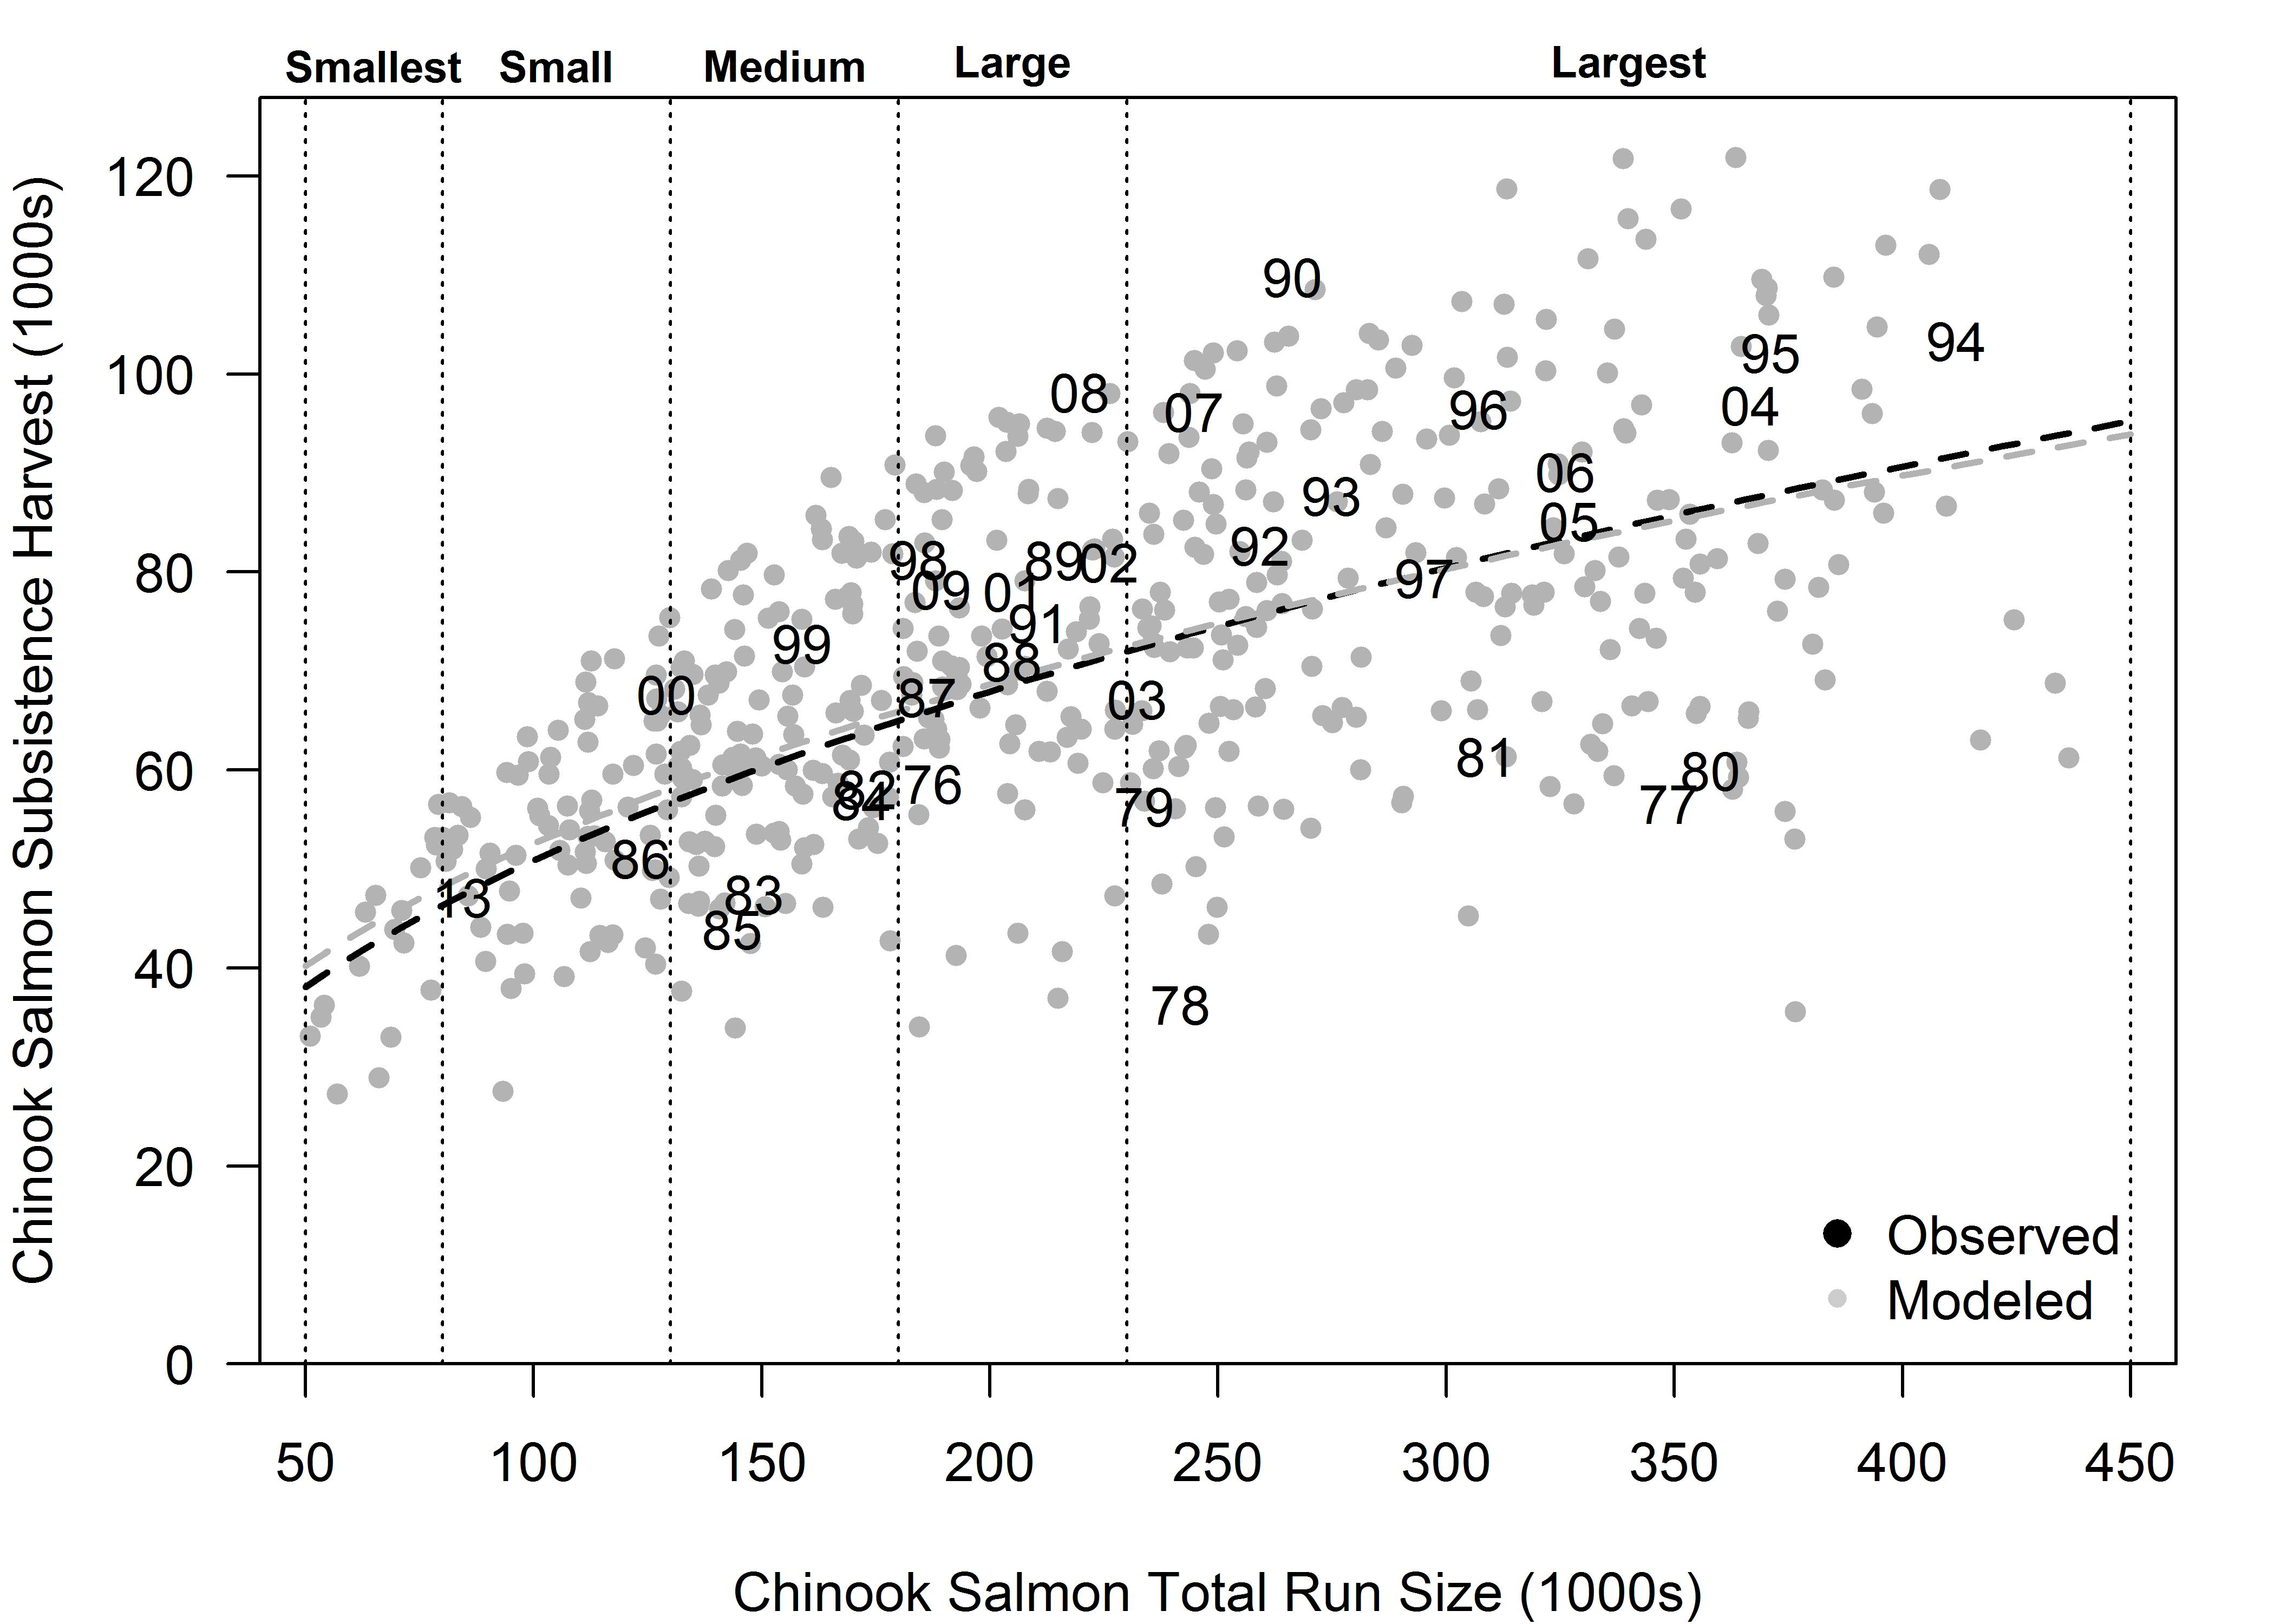
\includegraphics{img/Ch3/Figure B1.jpg}
  \caption{Observed and modeled Chinook salmon subsistence harvest as a function of total Chinook salmon run size. Individual black numbers are historical realizations in years with no harvest restrictions on the subsistence salmon fishery. Individual grey dots are modeled outcomes, each representing a hypothetical salmon run with different random subpopulation compositions, run timing, and species ratios. Fitted models display close agreement between the average simulated and observed harvest outcomes across the range of run sizes. Vertical dotted lines show the important run size strata used in this analysis.}
  \label{fig:HvN}
\end{figure}

\begin{figure}
  \centering
  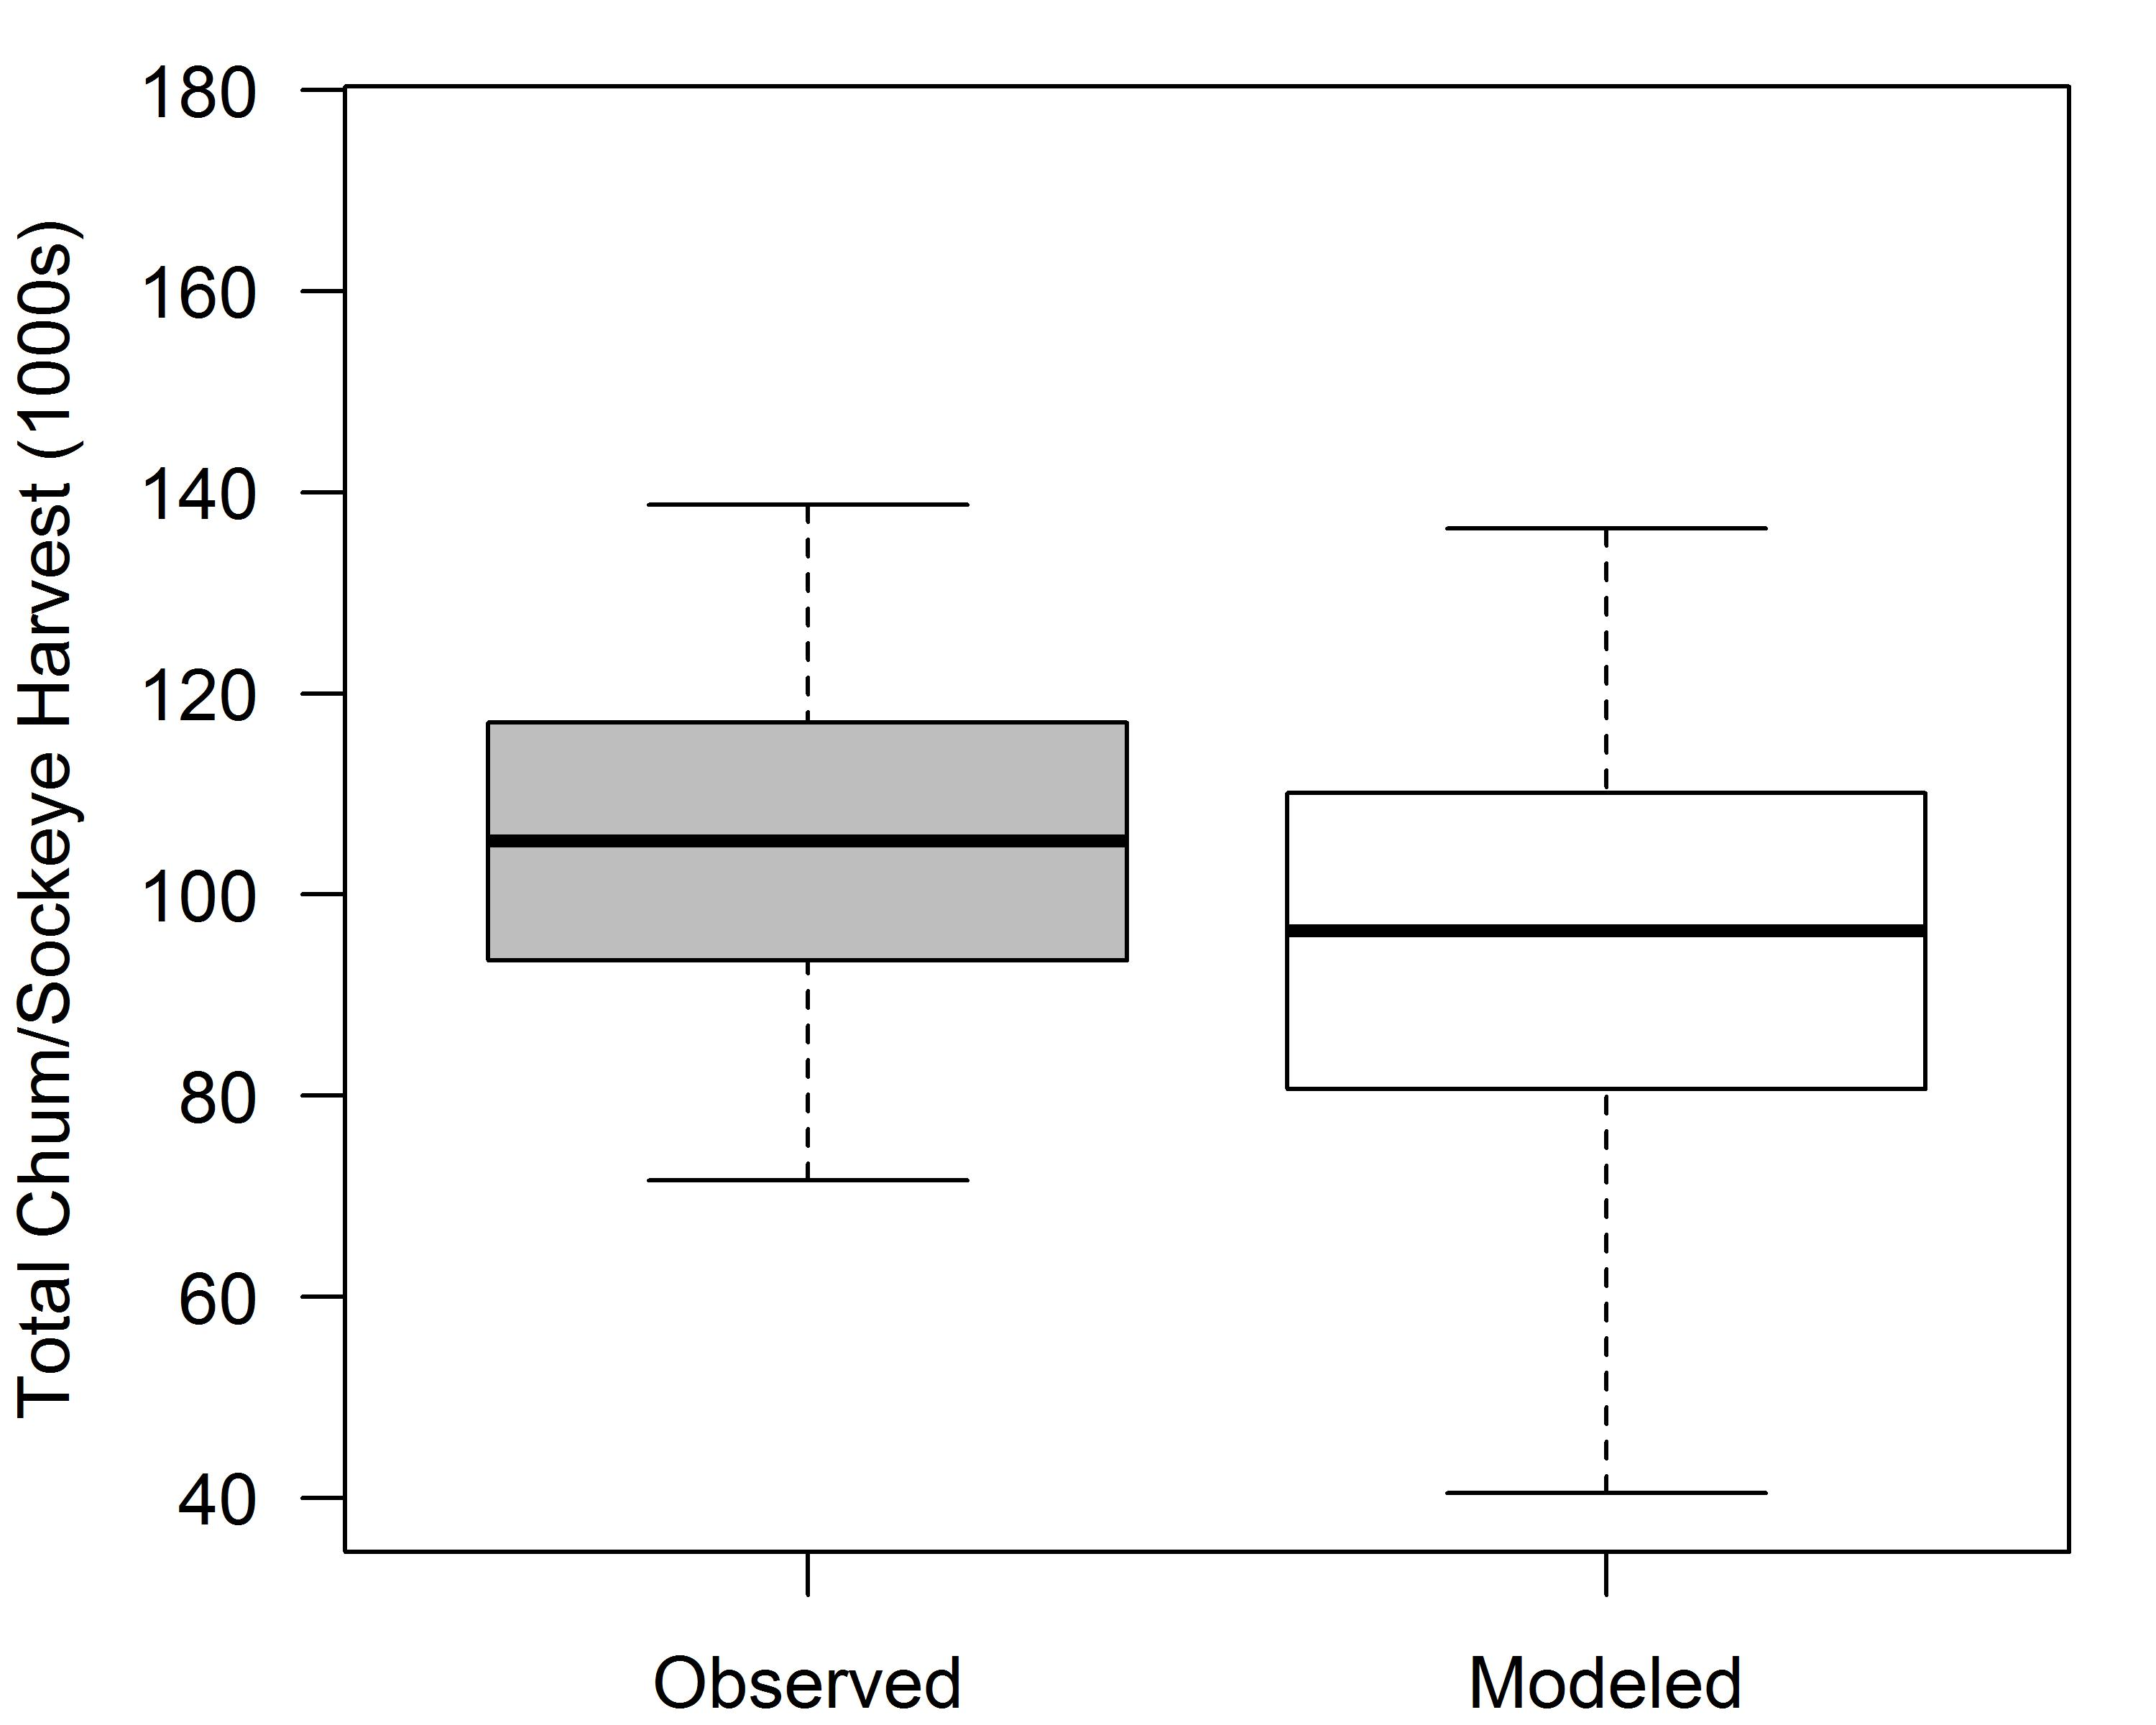
\includegraphics{img/Ch3/Figure B2.jpg}
  \caption{Comparison of the inter-annual distribution of observed and modeled chum/sockeye salmon harvests by villages located in the Kuskokwim River.}
  \label{fig:chsk-harvest}
\end{figure}

\clearpage

\begin{figure}
  \centering
  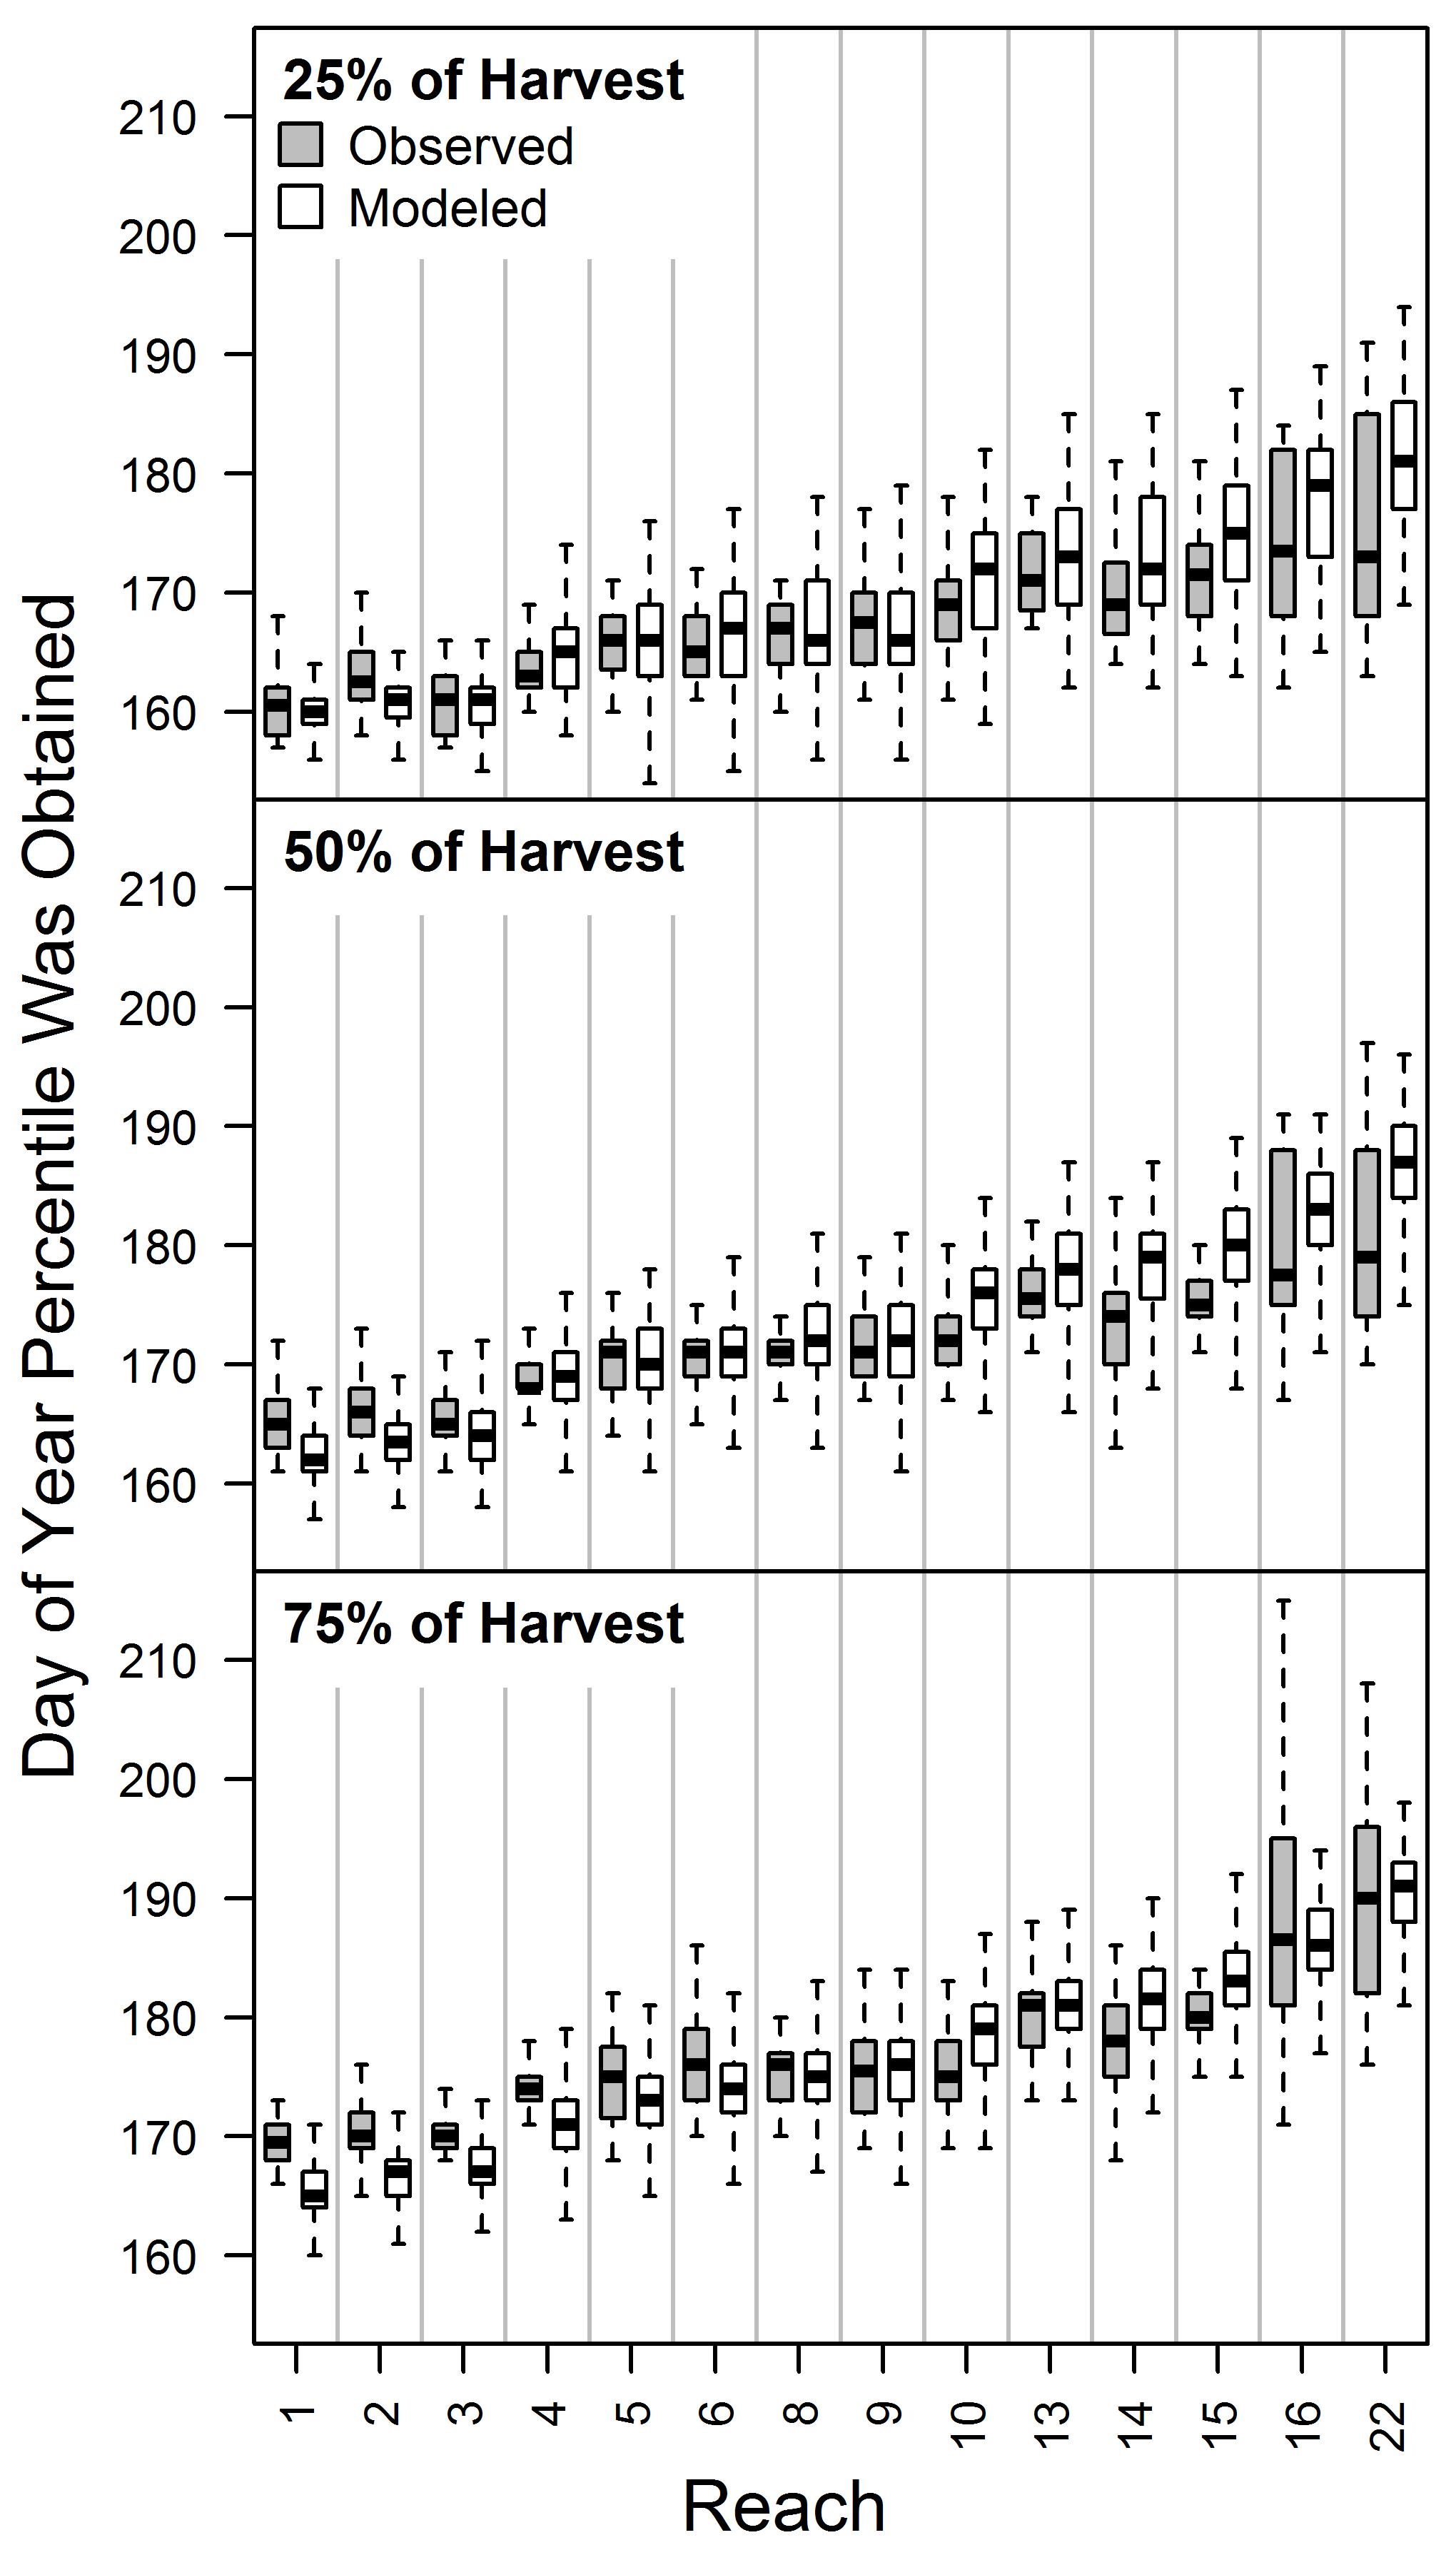
\includegraphics{img/Ch3/Figure B3.jpg}
  \caption{Comparison of the day of the year at which various percentiles of Chinook salmon harvest was attained by reach between observed and modeled outcomes. Variability in the observed boxplots is due to inter-annual variability in run size and timing and represents between-simulation variability for the modeled outcomes. Reach numbers are ordered from downriver to upriver. Note that not all reaches contain communities that harvest salmon.}
  \label{fig:temporal-harvest}
\end{figure}

\clearpage

\begin{figure}
  \centering
  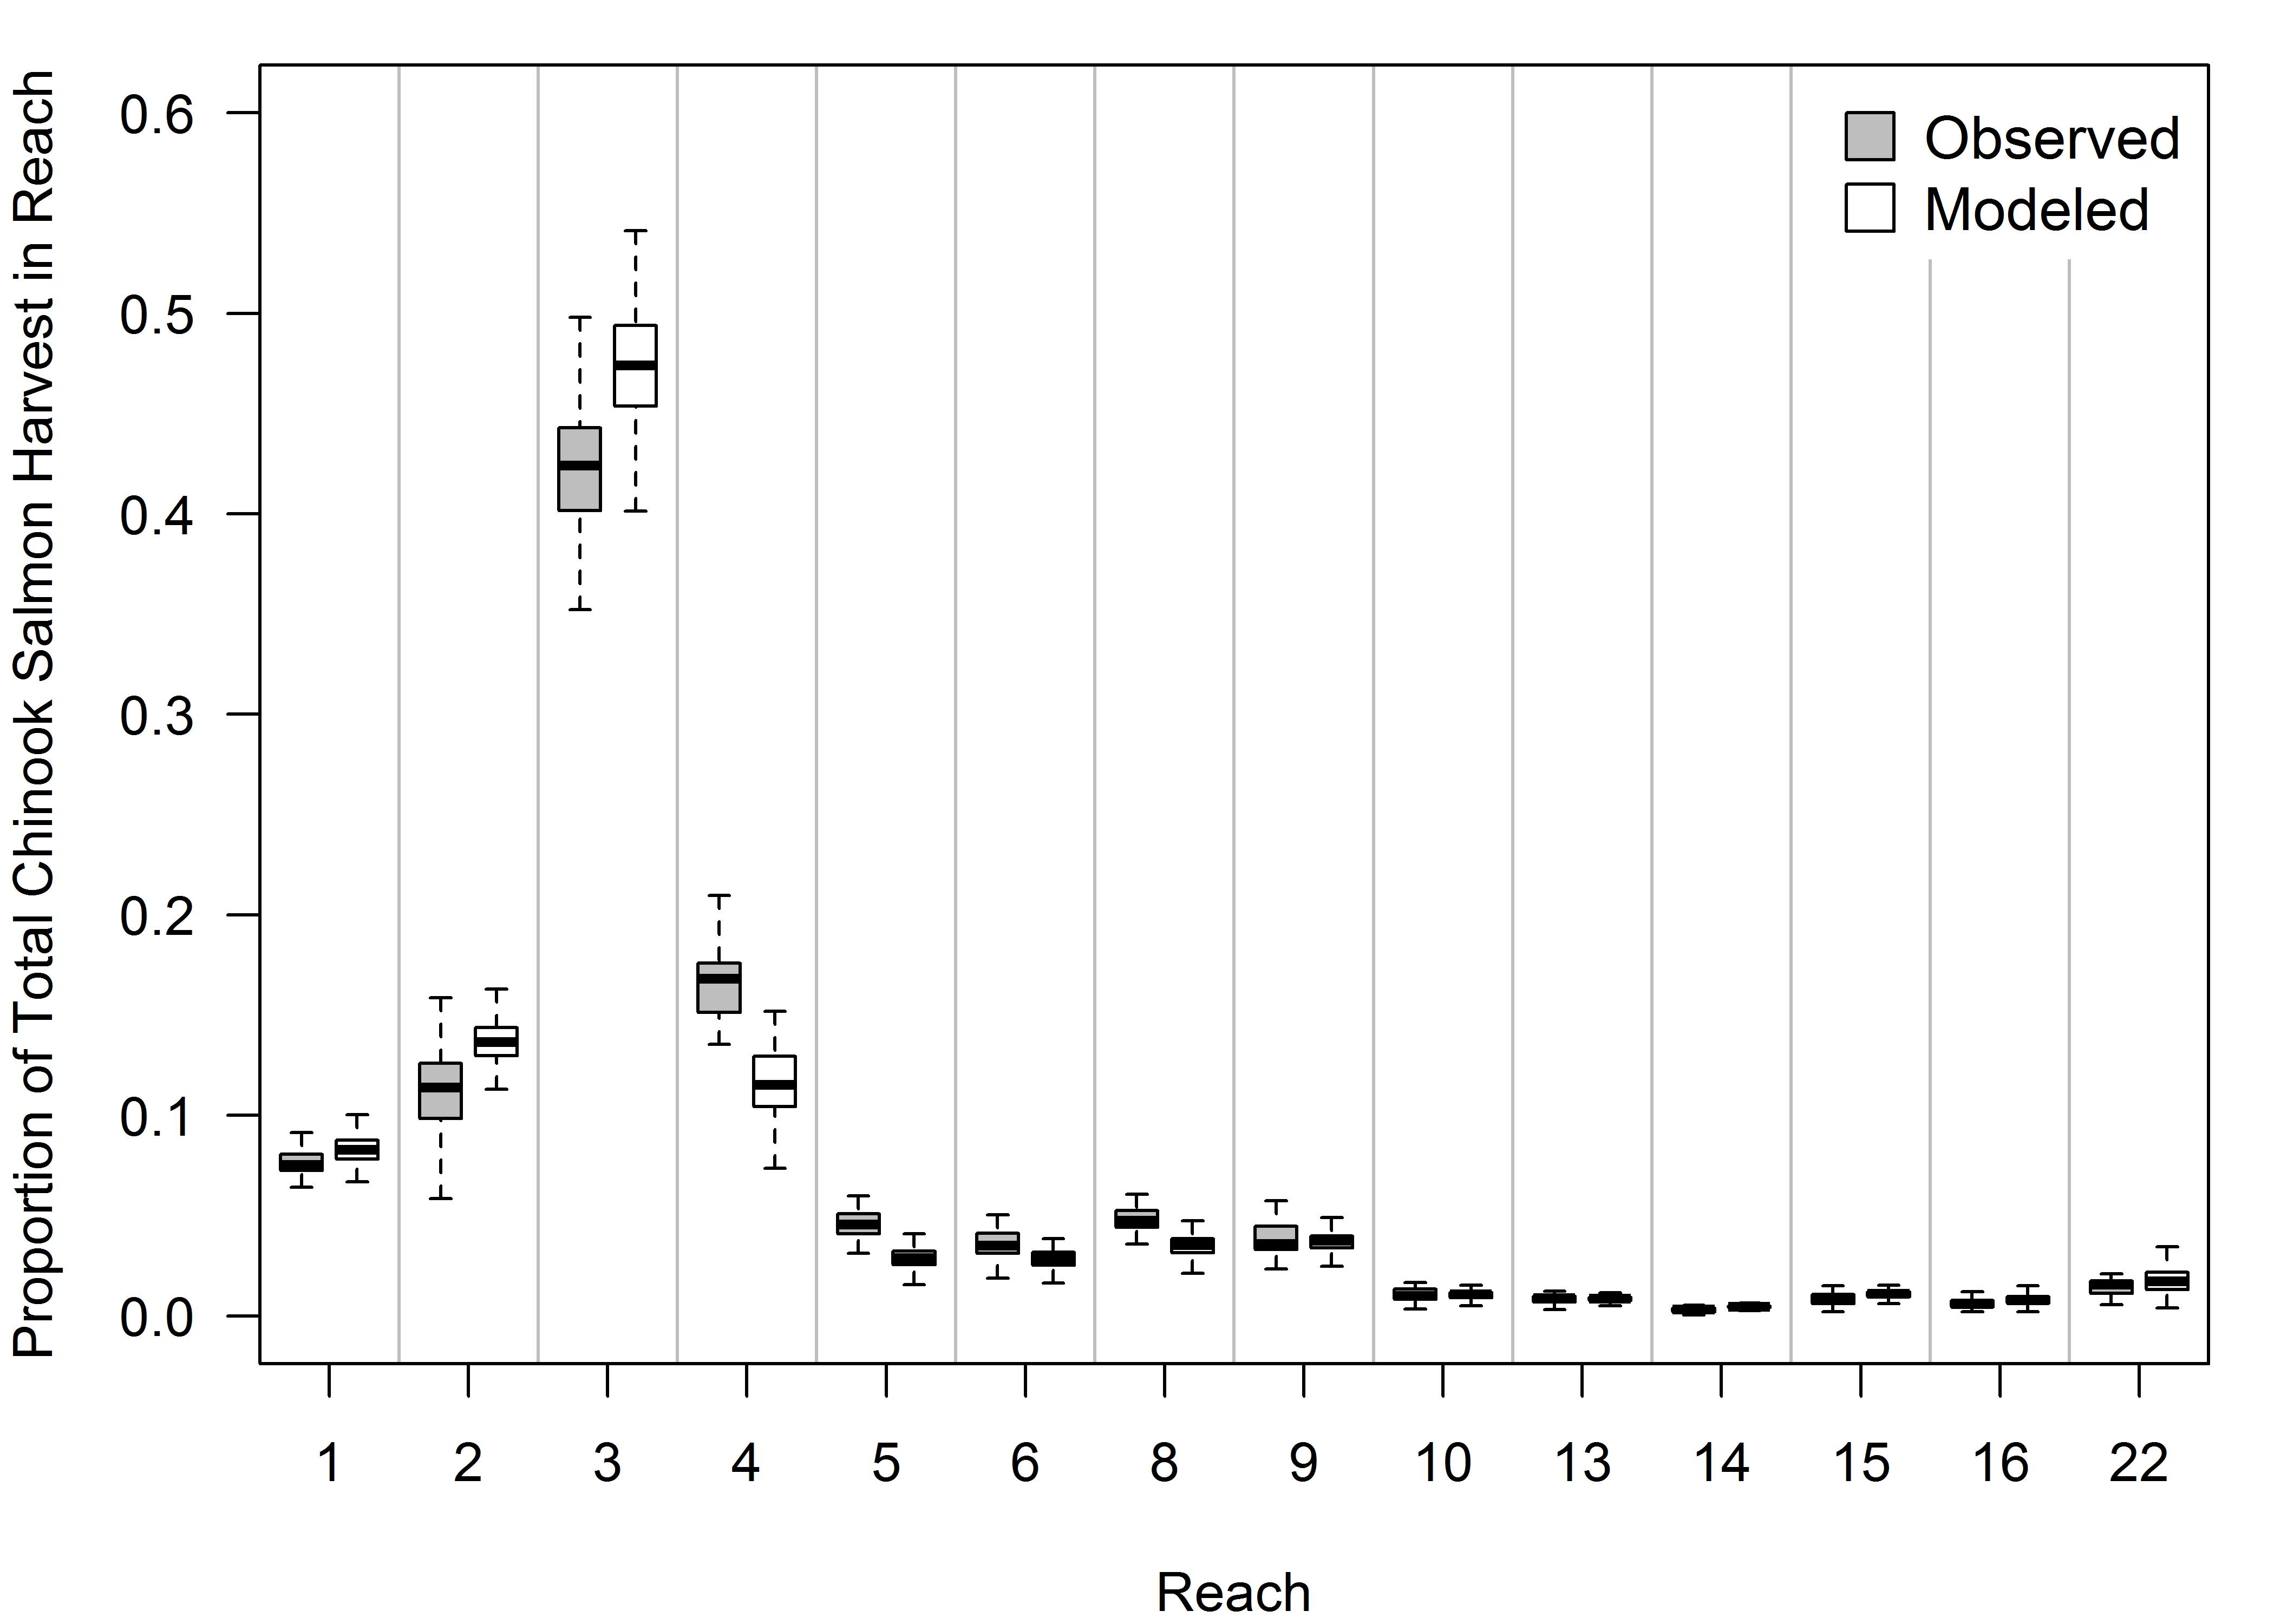
\includegraphics{img/Ch3/Figure B4.jpg}
  \caption{Comparison of the proportion of total drainage-wide Chinook salmon subsistence harvest attributable to communities in each reach between observed and modeled outcomes. Variability in the observed boxplots is due to inter-annual variability, and represents between-simulation variability for the modeled outcomes. Reach numbers are ordered from downriver to upriver. Note that not all reaches contain communities that harvest salmon.}
  \label{fig:spatial-harvest}
\end{figure}

\bibliography{cites-without-doi.bib,cites-with-doi.bib}


\end{document}
